On the Bayesian view, belief is not just a binary, on-off matter. Bayesians model agents not as simply categorically believing or disbelieving propositions, but rather as having \emph{degrees of confidence}, or \emph{degrees of belief}, or \emph{credences} in those propositions. Rather than flat out believing that your Kimchi Jjigae will turn out splendidly, you might, for example, be $0.7$ confident that it will turn out splendidly. Or you might have less precise opinions on the matter. You might be more confident than not that it will turn out splendidly. You might be at least $0.6$ confident and at most $0.9$ confident that it will turn out splendidly. You might have any number of more or less informative opinions, but nevertheless fall short of having a \emph{precise} credence on the matter. In that case, we say that your credences are \textit{imprecise}.

Credences, whether precise or imprecise, play a number of important theoretical roles according to Bayesians. For example, a rational agent's credences determine \textit{expectations} of measurable quantities---quantities like the size of the deficit $10$ years hence, or the utility of an outcome---which capture her \textit{best estimates} of those quantities. Those best estimates, in turn, typically \textit{rationalise} or make sense of her \textit{evaluative attitudes} and \textit{choice behaviour}.

Suppose that you are considering donating to charity. You have credences regarding the cost of bulk food, shipping, and other matters relevant for estimating how good different donation options are. Your credences, let's imagine, determine a higher expected utility for giving cash directly to the poor than for investing in infrastructure development. These expected utilities, on the Bayesian view, capture your best estimates of how much good each option would produce. And these best estimates, in turn, rationalise or make sense of your evaluative attitudes---your opinion that direct-giving is the better action, perhaps. Evaluative attitudes, in turn, rationalise choice behaviour. In the case at hand, your evaluative attitudes rationalise your choice to give cash directly to the poor rather than invest in infrastructure development.

According to many Bayesians, \textit{e.g.}, \citet{Koopman1940b, Koopman1940a}, \citet{Good1950}, \citet{deFinetti1951}, \citet{Savage1954}, and \citet{Joyce2010}, certain types of doxastic attitudes---opinions of the form ``X is at least as likely as Y,'' known as \textit{comparative beliefs}---play an especially important role in explicating the concept of credence. These explications typically involve an important bit of mathematics known as a \textit{representation theorem}. The aim of this chapter is straightforward, but fundamental. We will explore three very different approaches to explicating credence using comparative beliefs and representation theorems. Along the way, we will introduce a brand new account of credence: \textit{epistemic interpretivism}. We will also evaluate how these respective accounts stand up to the criticisms of \citet{Hajek2009b}, \citet{Meacham2011}, and \citet{Titelbaum2015}.

The rest of the chapter proceeds as follows. \autoref{konek-sec-1} outlines the main interpretations of \emph{comparative probability orderings}, which mirror the main interpretations of \emph{quantitative probability functions}. \autoref{konek-sec-2} homes in on one interpretation of comparative probability in particular: the \emph{subjectivist} interpretation. Then it briefly surveys some important representation theorems from \citet{Kraft1959}, \citet{Scott1964}, \citet{Suppes1976}, and \citet{Alon2014}. \autoref{konek-sec-3} outlines three different ``comparativist'' accounts of credence: the \textit{measurement-theoretic}, \textit{decision-theoretic}, and \textit{epistemic interpretivist} accounts. Comparativist accounts explain what it is to have one credal state or another in terms of subjective comparative probability relations (or comparative belief relations) and representation theorems. Epistemic interpretivism is an entirely new account of credence. So we spend a bit of time developing it. \autoref{konek-sec-4} examines criticisms of comparativist accounts by \citet{Hajek2009b}, \citet{Meacham2011}, and \citet{Titelbaum2015}. Finally, \autoref{konek-sec-5}, \autoref{konek-sec-6}, and \autoref{konek-sec-7} explore the extent to which our three different approaches can withstand these criticisms. We will pay special attention to the question of whether they vindicate \emph{probabilism}: the thesis that rational credences satisfy the probability axioms. 




\section{Main Interpretations of Comparative Probability}\label{konek-sec-1}



Probabilities seem to pop up all over the place. They feature in the respective explanations of all sorts of different phenomena. They help to explain, for example, \emph{singular events}, such as the outcomes of particular experiments, particular one-off historical events, and the like. Consider some examples:
\begin{enumerate}
\item[(1a)] Why did the die land with a blue face up?
\item[(1b)] It has $1$ blue faces and $1$ red face. And it's fair. So it had a $5/6$ probability of coming up blue.
\item[(2a)] Why did Rose get lung cancer?
\item[(2b)] She smoked for $30$ years. And the probability of getting lung cancer if you smoke for so long is really high.
\end{enumerate}
The high probability ($=5/6$) of this particular die coming up blue on this particular toss helps to explain why it in fact came up blue. And the high probability of this particular person---Rose---getting lung cancer (as a result of her $30$ years of smoking) helps to explain why she in fact got lung cancer. Probabilities also help to explain why we ought to have high or low confidence in certain hypotheses. Consider:
\begin{enumerate}
\item[(3a)] Why should we think that Quantum Electrodynamics is true?
\item[(3b)] It's the best confirmed physical theory ever. It's extremely probable given the current evidence.
\item[(4a)] Why should we think that Jones stole the paintings?
\item[(4b)] Given his acrimonious history with the art museum's curator, the eyewitness testimony, and the DNA evidence, it's quite probable that Jones is guilty.
\end{enumerate}
The extremely high probability of Quantum Electrodynamics given the current evidence at least partially explains why we ought to think that it is true. Likewise, the high probability that Jones stole the paintings given the eyewitness testimony, the DNA evidence, etc., at least partially explains why we ought to think that he is guilty. Finally, probabilities explain and rationalise our \emph{behaviour}. For example:
\begin{enumerate}
\item[(5a)] Why did you bet Aadil \textsterling$100$ that Manchester City would win their match against Newcastle?
\item[(5b)] Have you seen Newcastle lately? They're a joke. It's extremely probable that Manchester City will win.
\item[(6a)] Why did you go to Better Food Company rather than Sainsbury's?
\item[(6b)] I wanted fresh herbs, and it's more probable that the Better Food Company will have them.
\end{enumerate}
The fact that it is extremely probable, in your view, that Manchester City will win the match helps to explain why you took the bet. It also helps to rationalise or make sense of your decision. And the fact that it's more probable, in your view, that the Better Food Company will have fresh herbs than Sainsbury's helps to explain and rationalise your choice to go to the Better Food Company.

So, probabilities seem to do quite a lot of explanatory work. But no single thing is shouldering the whole explanatory load in (1)--(6). Different kinds of probability do the explaining in different examples. In (1)--(2), it is the \emph{physical probability} or \emph{chance} of the singular event in question that helps to explain why the event actually occurs. (See \citealp{Hajek2009b}, \citealp{Gillies2000}, and \citealp{Hitchcock2012}, for discussion of different theories of chance.) In (3)--(4), it is the \emph{logical probability} or \emph{degree of confirmation} of the hypothesis in question (conditional on the current evidence) that helps to explain why we ought to accept it. (See \citealp{Earman1992}, \citealp{Hajek2008}, and \citealp{Paris2011}, for discussion of Bayesian confirmation theory and some of its issues.) Finally, in (5)--(6), it is the \emph{subjective probability}, or \emph{degree of belief}, or \emph{credence}, of the agent in question that helps to explain and rationalise her choice.

Formally, a \emph{probability function} is just a particular type of real-valued function. Let $\Omega$ be a \emph{universal set}, which we can think of as the set of ``possible worlds'' or ``basic possibilities.'' And let $\F$ be a \emph{Boolean algebra} of subsets of $\Omega$, which we can think of as a set of ``propositions.'' More carefully, we can think of each $X\in\F$ as the proposition that is true at each world $w\in\F$, and false at each $w^*\not\in\F$. A Boolean algebra $\F$ of subsets of $\Omega$ has three important properties: (\emph{i}) $\F$ contains $\Omega$ (\emph{i.e.}, $\Omega\in\F$); (\emph{ii}) $\F$ is closed under complementation (\emph{i.e.}, if $X\in\F$, then $\Omega-X\in\F$); and (\emph{iii}) $\F$ is closed under unions (\emph{i.e.}, if $X,Y\in\F$, then $X\cup Y\in\F$). A real-valued function $p:\F\rightarrow\mathbb{R}$ is a \emph{probability function} if and only if it satisfies the laws of (finitely additive) probability.
\begin{enumerate}
\item\textsc{Normalization.}\, $p(\Omega)=1$.
\item\textsc{Nonnegativity.}\, $p(X)\geq p(\varnothing)$.
\item\textsc{Finite Additivity.}\, If $X\cap Y=\varnothing$, then $p(X\cup Y)=p(X)+p(Y)$.
\end{enumerate}
Axiom 1 says that $p$ must assign probability $1$ to the tautologous proposition $\Omega$. Axiom 2 says that $p$ must assign at least as high a probability to every proposition $X$ as it does to the contradiction $\varnothing$. Axiom 3 says that the probability that $p$ invests in a disjunction of incompatible propositions $X$ and $Y$ must be the sum of the probabilities that it invests in $X$ and $Y$, respectively.

The three main interpretations of probability---\emph{physical probability}, or \emph{chance}; \emph{logical probability}, or \emph{degree of confirmation}; and \emph{subjective probability}, or \emph{degree of belief}, or \emph{credence}---correspond to the three main types of phenomena that we use probability functions to model. For example, according to propensity theories of chance, chance functions measure how strongly a causal system is disposed to produce one outcome or other on a particular occasion. Chance functions, on this view, are just probability functions that are used to model one type of physical system (causal systems) as having one type of gradable property (causal dispositions of varying strengths). Likewise, logical probability functions measure how strongly a body of evidence $E$ supports or confirms a given hypothesis $H$. Logical probability functions are just probability functions that are used to model another type of target system (systems of propositions describing data and hypotheses) as having another type of gradable property (as having hypotheses which are supported to varying degrees by data propositions). Finally, subjective probability functions, or credence functions, measure (roughly) how confident an agent with some range of doxastic attitudes can be said to be of various propositions. Subjective probability functions are just probability functions that are used to model yet another type of system (an agent's doxastic attitudes) as having yet another type of gradable property (as either constituting or licensing varying degrees of confidence).

Of course, sorting out the precise relationship between these various models---probability functions---and their respective target systems is a delicate task. The ``interpretations'' above provide only rough, first-pass descriptions of that relationship. Part of this chapter's goal is to explore the relationship between \emph{subjective} probability functions, in particular, and the underlying system of doxastic attitudes that they model.

Just as there are a few main interpretations of \emph{quantitative probability functions}, corresponding to the main types of phenomena that we use those probability functions to model, so too are there a few main interpretations of ``comparative probability orderings.'' Formally, a comparative probability ordering is just particular type of relation $\succeq$ on a Boolean algebra $\F$ of subsets of $\Omega$. On each of the three main interpretations, ``$X\succeq Y$'' means roughly that \emph{X is at least as probable as Y}. (What \emph{exactly} this amounts to, however, will vary from interpretation to interpretation.) Traditionally, a relation $\succeq$ on $\F$ is said to be a \emph{comparative probability ordering} if and only if it satisfies de Finetti's (\citeyearhyper{deFinetti1964}, pp. 100--101) axioms of comparative probability.
\begin{enumerate}
\item \textsc{Nontriviality}.\, $\Omega\succeq \varnothing$ and $\varnothing\not\succeq \Omega$.
\item \textsc{Nonnegativity}.\, $X\succeq \varnothing$.
\item \textsc{Transitivity}.\, If $X\succeq Y$ and $Y\succeq Z$, then $X\succeq Z$.
\item \textsc{Totality}.\, $X\succeq Y$ or $Y\succeq X$.
\item \textsc{Quasi-Additivity}.\, If $X\cap Z=Y\cap Z=\varnothing$, then $X\succeq Y$ if and only if $X\cup Z\succeq Y\cup Z$.
\end{enumerate}
Axiom 1 says that the tautology $\Omega$ is strictly more probable than the contradiction $\varnothing$. Axiom 2 says that every proposition $X$ is at least as probable as the contradiction $\varnothing$. Axioms 3 and 4 guarantee that $\succeq$ is a total preorder (\textit{i.e.}, reflexive, transitive, and total). Finally, axiom 5 says that disjoining $X$ and $Y$ with some incompatible $Z$ does nothing to alter their comparative probability; so $X$ is at least as probable as $Y$ if and only if the disjunction of $X$ and $Z$ is at least as probable as the disjunction of $Y$ and $Z$.

The three main interpretations of comparative probability correspond to the three main types of phenomena that we use comparative probability orderings to model. \emph{Physical comparative probability orderings}, or \emph{chance orderings}---on one theory of chance anyway, \textit{viz.}, propensity theory---model causal systems. In particular, they model causal systems $\C$ as being more or less strongly disposed to produce one outcome or another on a particular occasion:
\begin{quote}
{\centering $X\succeq Y$\\
\textit{iff}\\}
$\C$ is at least as strongly disposed to produce an outcome $w\in X$ and thereby make $X$ true as it is to produce an outcome $w^*\in Y$ and thereby make $Y$ true.
\end{quote}
\emph{Logical comparative probability orderings} model a rather different type of target system: systems of propositions describing data and hypotheses. In particular, they model certain data $D$ as supporting or confirming certain hypotheses $H$ more than other data $D^*$ support other hypotheses $H^*$:
\begin{quote}
{\centering
$\left<H,D\right>\succeq \left<H^*,D^*\right>$\\
\textit{iff}\\}
$D$ supports or confirms $H$ at least as much as $D^*$ supports or confirms $H^*$.
\end{quote}
Finally, \emph{subjective comparative probability orderings} model yet another type of target system: an agent's doxastic attitudes. In particular, they model agent $\A$ as being more or less confident that one proposition or another is true:
\begin{quote}
{\centering
$X\succeq Y$\\
\textit{iff}\\}
$\A$ is at least as confident that $X$ is true as she is that $Y$ is true.
\end{quote}

Of course, the three main interpretations of comparative probability are really \emph{families} of interpretations. All three types of comparative probability orderings come in different flavours. For example, behaviorists like \citet{deFinetti1931, deFinetti1964} and \citet{Savage1954} treat subjective comparative probability orderings as particular types of \emph{preference orderings}. To be more confident that $X$ is true than $Y$ is, roughly speaking, to prefer a dollar bet on $X$ to a dollar bet on $Y$. They subscribe to what Jeffrey calls \emph{the thesis of the primacy of practical reason}, which says that between belief and preference, ``it is preference that is real and primary'' \citep[p. 590]{Jeffrey1987}. Hence, ``belief states that correspond to identical preference rankings of propositions are in fact one and the same'' \citep[p. 138]{Jeffrey1983}.


\citet{Jeffrey1965, Jeffrey2002} and \citet{Joyce1999}, in contrast, do not subscribe to this thesis. On their view, being more confident that $X$ is true than $Y$ involves making a peculiarly \emph{doxastic} judgment. Such doxastic judgments partially explain and rationalise our preferences. But they do not even supervene on preferences, let alone reduce to them. (Two agents, for example, could both be in a state of nirvana on this view, and so be indifferent between every prospect and the status quo, but nevertheless make different comparative probability judgments.) And the laws governing \emph{rational} subjective comparative probability judgments, on this account, are not simply special cases of the laws governing rational preference. Rather, they derive from peculiarly \emph{epistemic} considerations, \textit{e.g.}, considerations of \emph{accuracy}.

To have a general way of talking about comparative beliefs, without assuming that they satisfy de Finetti's axioms, let's introduce some terminology. Call any relation $\succeq$ on an algebra $\F$ of subsets of $\Omega$ that is used to model an agent's comparative beliefs a \emph{comparative belief relation}. And call $\left<\Omega,\F,\succeq\right>$ a \emph{comparative belief structure}. Comparative belief relations may or may not be comparative probability orderings. That is, they may or may not satisfy de Finetti's axioms of comparative probability.

Why the hubbub about comparative belief? Why think that comparative belief relations have a particularly important role to play in modeling rational agents' doxastic states? What are they especially suited to do that precise, real-valued credence functions are not?


There are a number of common answers to these questions. The first is that comparative belief relations provide a more psychologically realistic model of agents' doxastic attitudes than precise, real-valued credence functions. Often I simply lack an opinion about which of two propositions is more plausible. I am not \textit{more} confident that copper will be greater than \textsterling$2$/lb in 2025 (call this proposition $C$) than I am that nickel will be greater than \textsterling$3$/lb in 2025 (call this proposition $N$). Neither am I \textit{less} confident in $C$ than $N$, nor \textit{equally} confident. I simply lack an opinion on the matter. We can model this using comparative belief relations. Just choose a relation $\succeq$ that does not rank $C$ and $N$:
$$ C\not\succeq N\hspace*{2mm}\textrm{and}\hspace*{2mm}N\not\succeq C. $$
The incompleteness in $\succeq$ reflects my lack of opinionation. Precise credence functions, on the other hand, do not allow for this sort of lack of opinionation. \textit{Any} agent with precise credences for $C$ and $N$ takes a stand on their comparative plausibility. She is either more confident in $C$ than $N$, less confident in $C$ than $N$, or equally confident in the two.\footnote{See \citet[p. 19]{Suppes1994}, \citet[p. 325]{Kyburg1996}, \citet[p. 47]{Kaplan2010}, and \citet[p. 283]{Joyce2010} for similar remarks.}




The second answer is \textit{evidentialist}. Not only do real agents \textit{in fact} have sparse and incomplete opinions, but they \textit{ought} to have such opinions. If your evidence is incomplete and unspecific, then your comparative beliefs (and your other qualitative and comparative opinions) should be correspondingly incomplete to reflect the unspecific nature of that evidence. This is the response that is most \textit{justified}, or \textit{warranted}, or \textit{appropriate} in light of such evidence. Again, we can capture this sort of lack of opinionation using comparative belief relations, but not using precise credence functions. Having precise credences requires having total or complete comparative beliefs (as well as total conditional comparative beliefs, total preferences, and so on).\footnote{See \citet[p. 171]{Joyce2005} for similar remarks.}



The third answer is \textit{information-theoretic}. Proponents of maximum entropy methods, for example, argue that you ought to have the \textit{least informative} doxastic state consistent with your evidence. And according to any plausible informativeness or entropy measure for comparative beliefs, any incomplete comparative belief relation will be less informative than any extension of it.\footnote{See \citet{Abellan2000,Abellan2003} for measures of entropy for imprecise probability models which might also serve as measures of entropy for comparative belief relations.} As a result, minimizing informativeness will often require adopting incomplete comparative beliefs. Precise credences, however, do not allow for incomplete comparative beliefs. As Joyce puts it, adopting precise credences, in many evidential circumstances, ``amounts to pretending that you have lots and lots of information that you simply don't have'' \citep[p. 284]{Joyce2010}.

The final common answer is that comparative belief is more explanatorily fundamental than precise credence. Comparative beliefs figure into the best explanation of \textit{what precise credences are}, but not vice versa. It is worthwhile, then, exploring the various accounts of credence that aim to furnish such an explanation. We will turn our attention to them shortly. Each of these accounts, however, makes use of an important bit of mathematics known as a \textit{representation theorem}. So our first task is to get familiar with the nuts and bolts of representation theorems.






\section{Representation Theorems}\label{konek-sec-2}


Suppose that Monty Hall invites you to choose one of three doors: either door $a$, $b$, or $c$. Behind one of these doors: a car. Behind the other two: a goat. You are more confident that the car is behind $a$ than $b$, let's imagine. You are also more confident that it's behind $b$ than $c$. But that is all. You do not take a stand, for example, on whether it's more likely to be behind either $b$ or $c$ than $a$, or vice versa. You abstain from judgment on all other matters.

Let $w_a$ be the world in which the car is behind door $a$, $w_b$ be the world in which the car is behind door $b$, and $w_c$ be the world in which the car is behind door $c$. Then we can represent you as having comparative beliefs about propositions in the following Boolean algebra:
$$
\F = \left\{
	\begin{tabular}{c}
		$\left\{w_a,w_b,w_c\right\}$\\
		$\left\{w_a,w_b\right\}, \left\{w_a,w_c\right\}, \left\{w_b,w_c\right\},$\\
		$\left\{w_a\right\}, \left\{w_b\right\}, \left\{w_c\right\},$\\
		$\varnothing$\\
	\end{tabular}
\right\}.
$$
And we can represent those fragmentary comparative beliefs as follows:
$$
\left\{w_a,w_b,w_c\right\}\succ\left\{w_a\right\}\succ\left\{w_b\right\}\succ\left\{w_c\right\}\succ\varnothing,
$$
where $X\succ Y$ is shorthand for $X\succeq Y$ and $X\not\preceq Y$.\footnote{This shorthand is inadequate. You may well think $X\succeq Y$ and $X\not\preceq Y$ without thinking $X\succ Y$. Imagine for example that you recently learned that $Y$ entails $X$. So you think that $X$ is at least as likely as $Y$, \textit{i.e.}, $X\succeq Y$. But you have no idea whether the entailment goes both ways. So you withhold judgment about whether $Y$ is at least as likely as $X$, \textit{i.e.}, $X\not\preceq Y$. For exactly the same reason you withhold judgment about whether $X$ is strictly more likely than $Y$, \textit{i.e.}, $X\not\succ Y$. We would do better, then, to represent your doxastic state with a \emph{pair} of relations $\left<\succ, \succeq\right>$. But historically one or the other has been taken as primitive. For ease of exposition, we follow \citet{deFinetti1951}, \citet{Savage1954}, and \citet{Krantz1971}, who take $\succeq$ as primitive.} 


Your comparative belief relation $\succeq$ is \textit{not} a comparative probability ordering, \textit{i.e.}, $\succeq$ does not satisfy de Finetti's axioms of comparative probability. Relation $\succeq$ violates Quasi-Additivity, for example, as well as totality. You are, after all, more confident that the car is behind $a$ than $b$: 
$$ \left\{w_a\right\}\succ\left\{w_b\right\}. $$
So de Finetti's Quasi-Additivity axiom demands that you also be more confident that it is behind $a$ or $c$ than you are that it is behind $b$ or $c$. But you abstain from judgment on the matter: 
$$ \left\{w_a,w_c\right\}\not\succeq\left\{w_b,w_c\right\}\hspace*{2mm}\textrm{and}\hspace*{2mm}\left\{w_a,w_c\right\}\not\preceq\left\{w_b,w_c\right\}. $$
A few back-of-the-envelope calculations suffice to show that de Finetti's axioms are necessary for \textit{probabilistic representability}. Following \citet{Savage1954}, we say that:
\begin{quote}\centering
$p$ \emph{fully agrees} with $\succeq$\\
\textit{iff}\\
$X\succeq Y \Leftrightarrow p(X)\geq p(Y)$.
\end{quote}
We say that $\succeq$ is (fully) \emph{probabilistically representable} iff there is a probability function $p$ that fully agrees with $\succeq$. Since your comparative belief relation $\succeq$ does not satisfy de Finetti's axioms, in our little example, it is not probabilistically representable.

De Finetti (\citeyear{deFinetti1951}) famously conjectured that his axioms encode not only necessary conditions for probabilistically representability, but \textit{sufficient} conditions as well. The question: was de Finetti right?

Let $\left<\Omega,\F,\succeq\right>$ be an agent's comparative belief structure. (For now, assume that $\F$ is finite.) Probability functions that fully agree with $\succeq$ show that we can think of that structure $\left<\Omega,\F,\succeq\right>$ numerically, so to speak. We can map the propositions $X$ in $\F$ to real-valued proxies $p(X)$. And we can do so in such a way that one proxy $p(X)$ is larger than another $p(Y)$ exactly when our agent is more confident in $X$ than $Y$. So the familiar ``greater than or equal to'' relation $\geq$ on the real numbers $\mathbb{R}$ is a mirror image of our agent's comparative belief relation $\succeq$ on $\F$.

\citet{Kraft1959} show that de Finetti's conjecture is false. Though de Finetti's axioms are \emph{necessary} for probabilistic representability, they are not \emph{sufficient}. To establish this, \citeauthor{Kraft1959} construct a clever counterexample involving a comparative belief relation $\succeq$ over the Boolean algebra $\G$ of all subsets of $\Omega=\left\{w_a,w_b,w_c,w_d,w_e\right\}$. Their relation $\succeq$ satisfies de Finetti's axioms of comparative probability, and also the following inequalities:
\begin{align}\label{eq:1-3}
		\left\{w_d\right\} & \succ  \left\{w_a,w_c\right\},\\
		\left\{w_b,w_c\right\} & \succ  \left\{w_a,w_d\right\},\\
		\left\{w_a,w_e\right\} & \succ \left\{w_c,w_d\right\}.
	\end{align}	
As a result, any probability function $p$ that fully agrees with $\succeq$ satisfies the corresponding inequalities (to simplify notation, we let $p(\left\{w\right\})=p(w)$):
\begin{align}\label{eq:4-6}
		p(w_d) & >  p(w_a)+p(w_c),\\
		p(w_b)+p(w_c) & > p(w_a)+p(w_d),\\
		p(w_a)+p(w_e) & > p(w_c)+p(w_d).
	\end{align}	
But any $p$ that satisfies (4)--(6) also satisfies (7) (simply sum the inequalities).
\begin{align}\label{eq:7}
		p(w_b)+p(w_e) & > p(w_a)+p(w_c)+p(w_d).
	\end{align}	
Notice, however, that $\left\{w_b,w_e\right\}$ and $\left\{w_a,w_c,w_d\right\}$ appear nowhere in (1)--(3). So Transitivity does not constrain how you order them. Neither do any supersets of $\left\{w_b,w_e\right\}$ or $\left\{w_a,w_c,w_d\right\}$ appear there. So Quasi-Additivity does not constrain how you order them either. Hence, for all de Finetti's axiom say, you can order $\left\{w_b,w_e\right\}$ and $\left\{w_a,w_c,w_d\right\}$ any way you please. So \citeauthor{Kraft1959} make $\succeq$ satisfy (8).
\begin{align}\label{eq:8}
		\left\{w_b,w_e\right\} & \preceq \left\{w_a,w_c,w_d\right\}.
	\end{align}
But if $p$ fully agrees with $\succeq$, then (8) requires:
\begin{align}\label{eq:9}
		p(w_b)+p(w_e) & \leq p(w_a)+p(w_c)+p(w_d).
	\end{align}
Lines (7) and (9), however, are jointly unsatisfiable. So no probability function $p$ fully agrees with $\succeq$.



\subsection{Scott's Theorem}


So de Finetti's conjecture is false. De Finetti's axioms of comparative probability are \textit{not} necessary and sufficient for probabilistic representability. Luckily, \citet{Kraft1959} and \citet{Scott1964} provide the requisite fix. They provide stronger axioms that are both necessary and sufficient for probabilistic representability. Scott's axioms are more straightforward, so we will focus our attention on them. 

Before stating Scott's theorem, it is worth noting that our formulation abuses notation a bit. Expressions `$X_i$' and `$Y_i$' refer both to propositions in $\F$, as well as their characteristic functions, \textit{i.e.}, functions that take the value $1$ at worlds $w$ where $X_i$ (or $Y_i$) is true (\textit{i.e.}, $w\in X_i$), and take the value $1$ at worlds $w^\prime$ where $X_i$ is false (\textit{i.e.}, $w^\prime\not\in X_i$). This will turn out to be a helpful bit of sloppiness. 


\citet{Scott1964} proves the following: 
\begin{quote}
\textbf{Scott's Theorem}. Every comparative belief structure $\left<\Omega,\F,\succeq\right>$ (with finite $\F$) has a probability function $p:\F\rightarrow\mathbb{R}$ that fully agrees with $\succeq$ in the sense that
\[
X\succeq Y \Leftrightarrow p(X)\geq p(Y)
\]
if and only if $\succeq$ satisfies the following axioms.
\begin{enumerate}
\item \textsc{Non-triviality}.\, $\Omega\succ \varnothing$.
\item \textsc{Non-negativity}.\, $X\succeq \varnothing$.
\item \textsc{Totality}.\, $X\succeq Y$ or $Y\succeq X$.
\item \textsc{Isovalence}.\, If $X_1+\ldots+X_n=Y_1+\ldots+Y_n$ and $X_i\succeq Y_i$ for all $i\leq n$, then $X_i\preceq Y_i$ for all $i\leq n$ as well.
\end{enumerate}
\end{quote}
Axiom 4---sometimes called \textit{Scott's axiom}, the \textit{Isovalence axiom}, or the \textit{Finite cancellation axiom}---is the one new axiom of the bunch. To see what it says, note that $X_1(w)+\ldots+X_n(w)$ counts the number of truths in the set $\left\{X_1,\hdots,X_n\right\}$ at world $w$. Ditto for $Y_1(w)+\ldots+Y_n(w)$. So
\[
X_1+\ldots+X_n=Y_1+\ldots+Y_n
\]
says that the two sets of propositions, $\left\{X_1,\hdots,X_n\right\}$ and $\left\{Y_1,\hdots,Y_n\right\}$, contain the same number of truths \textit{come what may}, \textit{i.e.}, in every possible world. We call such sets of propositions  \textit{isovalent}.

In light of this, the Isovalence axiom says that if $\left\{X_1,\hdots,X_n\right\}$ and $\left\{Y_1,\hdots,Y_n\right\}$ are isovalent, then you cannot think that the $X_i$s are uniformly more plausible than the $Y_i$s. (``Uniformly more plausible'' here means that you think that $X_i$ is at least as plausible as $Y_i$ for all $i$, and that $X_j$ is strictly more plausible than $Y_j$ for some $j$.) After all, an equal number of the $X_i$s and $Y_i$s are \textit{guaranteed} to be true! So you can only think that the $X_i$s are at least as plausible as the $Y_i$s across the board if you think that they are \textit{equally plausible}.

But how exactly does Scott \textit{prove} his representation theorem? It is worth walking through the proof strategy informally. This will help interested readers dig through the mathematical minutia in \citet{Scott1964}.

Indeed, it will prove instructive to use Scott's strategy to establish something slightly stronger than Scott's theorem.
\begin{quote}
\textbf{Generalised Scott's Theorem (GST)}. For any comparative belief structure $\left<\Omega,\F,\succeq\right>$ with finite $\F$ and a comparative belief relation $\succeq$ that satisfies 
\begin{enumerate}
\item \textsc{Non-triviality}.\, $\Omega\succ \varnothing$,
\item \textsc{Non-negativity}.\, $X\succeq \varnothing$,
\end{enumerate}
the following two conditions are equivalent.
\begin{enumerate}
\item[3.] \textsc{Isovalence}.\, If $X_1+\ldots+X_n=Y_1+\ldots+Y_n$ and $X_i\succeq Y_i$ for all $i\leq n$, then $X_i\preceq Y_i$ for all $i\leq n$ as well.
\item[4.] \textsc{Strong representability}.\, there exists a probability function $p:\F\rightarrow\mathbb{R}$ that \textit{strongly agrees} with $\succeq$ in the sense that
\begin{enumerate}
\item[(i)] $X\succeq Y \Rightarrow p(X)\geq p(Y)$,
\item[(ii)] $X\succ Y \Rightarrow p(X)>p(Y)$.
\end{enumerate}
\end{enumerate}
\end{quote}
Scott's theorem, as we shall see at the end of \autoref{konek-sec-2}, follows fairly straightforwardly from GST. We prove the GST in the appendix.

The key insight required for proving GST is this. In the presence of Non-triviality and Non-negativity, strong representability boils down to sorting \textit{almost desirable gambles} from \textit{undesirable gambles}.\footnote{For an accessible introduction to desirable gambles, see \citet{Walley2000}. See \citet{Quaeghebeur2014} for more detail.} On top of this, \citet{Scott1964} shows that sorting almost desirable from undesirable gambles is equivalent to satisfying Isovalence.\footnote{More carefully, \citet{Scott1964} shows that for any comparative belief relation $\succeq$ that satisfies Non-triviality and Non-negativity, satisfying Isovalence is \textit{sufficient} for sorting almost desirable from undesirable gambles. Showing that it is \textit{necessary} is straightforward. See the appendix for proof.} \autoref{konek-fig-1} summarizes the situation.
\begin{figure}[ht]
\centering
\vspace*{3mm}
\fbox{\parbox[t]{3
in}{

\centerline{\textit{Given Non-triviality and Non-negativity}}

\vspace*{3mm}
\centerline{\fbox{Strong rep.}$\Leftrightarrow$\fbox{Sort gambles}$\Leftrightarrow$\fbox{Isovalence}}}}
\caption{Logical relations between properties of $\succeq$}\label{konek-fig-1}
\end{figure}

Gambles are measurable quantities $\G:\Omega\rightarrow\mathbb{R}$. Say that a gamble $\G$ is \textit{almost desirable} relative to $\succeq$ iff it is a non-negative linear combination of almost desirable components:
$$ (X_1-Y_1),\hdots,(X_n-Y_n). $$
And say that each component $X_i-Y_i$ is almost desirable iff $X_i\succeq Y_i$. Gamble $\G$ is a non-negative linear combination of $(X_1-Y_1),\hdots,(X_n-Y_n)$ just in case:
$$ \G=\sum_i \lambda_i(X_i-Y_i) $$
for some $\lambda_1,\hdots,\lambda_n\geq0$.

We call components $X_i-Y_i$ almost-desirable if $X_i\succeq Y_i$ because any probability function $p$ that strongly agrees with $\succeq$ determines a non-negative expected value for $X_i-Y_i$:
\begin{eqnarray*}
X_i\succeq Y_i & \Rightarrow & p(X_i)\geq p(Y_i)\\
& \Leftrightarrow & E_p[X_i]\geq E_p[X_i]\\
& \Leftrightarrow & E_p[X_i-Y_i]\geq 0.
\end{eqnarray*}
So if we interpret those values as payoffs in utility, then $p$ expects $X_i-Y_i$ to be at least as good as the status quo (\textit{i.e.}, its expected utility is non-negative).

Likewise, we call $\G$ almost desirable if it is a non-negative linear combination of almost-desirable components because any probability function $p$ that strongly agrees with $\succeq$ determines a non-negative expected value for $\G$:
\begin{eqnarray*}
X_i\succeq Y_i\hspace*{2mm}\text{ for all } i & \Rightarrow & E_p[X_i-Y_i]\geq 0\hspace*{2mm}\text{ for all } i\\
& \Rightarrow & \sum_i \lambda_iE_p[X_i-Y_i]\geq 0\\
& \Leftrightarrow & E_p\left[\sum_i \lambda_i(X_i-Y_i)\right]\geq 0\\
& \Leftrightarrow & E_p[\G]\geq 0.
\end{eqnarray*}
Similar remarks apply to \textit{undesirable gambles}. We call a gamble $\G^*$ \textit{undesirable} relative to $\succeq$ iff it is a convex combination of undesirable components
$$ (X^*_1-Y^*_1),\hdots,(X^*_n-Y^*_n), $$
so that 
$$ \G^*=\sum_i \lambda^*_i(X^*_i-Y^*_i). $$
for some $\lambda^*_1,\hdots,\lambda^*_n\geq0$ with $\sum_i \lambda^*_i=1$. A component $X^*_i-Y^*_i$ is undesirable iff $X^*_i\prec Y^*_i$. The reason is the same as before. Any probability function that strongly agrees with $\succeq$ determines a negative expected value for undesirable components, as well as convex combinations of undesirable components.

Now say that $\succeq$ \textit{sorts almost desirable gambles from undesirable ones} iff the two sets of gambles are disjoint. That is, if
$$ \mathbb{A}=\left\{\G \mathrel{|} \G \text{ is almost desirable rel. to } \succeq \right\} $$
and
$$ \mathbb{U}=\left\{\G^* \mathrel{|} \G^* \text{ is undesirable rel. to }\succeq\right\}, $$
then $\succeq$ sorts almost desirable gambles from undesirable ones iff
$$ \mathbb{A}\cap\mathbb{U}=\varnothing. $$

If $\succeq$ fails to sort gambles in this way, then some gamble is both almost desirable and undesirable, \textit{i.e.}, $\G=\G^*$ for some almost desirable gamble $\G$ and some undesirable gamble $\G^*$. And if \textit{that} is the case, then there is no probability that \textit{strongly} agrees with it. (Moreover, since full probabilistic representability entails strong representability, there is no probability function that fully agrees with it either.) If it \textit{were} strongly representable, then we would have both
$$ E_p[\G]=E_p[\G^*] $$
and
$$ E_p[\G^*]<0\leq E_p[\G] $$
for some probability function $p$.

This shows that sorting almost desirable from undesirable gambles is \textit{necessary} for strong agreement with a probability function, which is itself \textit{necessary} for full agreement with a probability function, \textit{i.e.}, probabilistic representability. Scott's insight, though, is that it is also \textit{sufficient}, in the presence of Non-triviality and Non-negativity. Given that $\succeq$ satisfies Non-triviality and Non-negativity, it sorts almost desirable from undesirable gambles \textit{if and only if} it strongly agrees with a probability function. What's more, if $\succeq$ is total as well, then \textit{strong} agreement is equivalent to \textit{full} agreement. So non-trivial, non-negative, total comparative belief relations sort almost desirable from undesirable gambles \textit{if and only if} they are probabilistically representable. See \autoref{konek-fig-2}.

\begin{figure}
\centering
\fbox{\parbox[t]{3.2in}{\begin{center}
\textit{Given Non-triviality, Non-negativity and Totality}

\vspace*{3mm}

\fbox{Strong rep.}$\Leftrightarrow$\fbox{Full prob. rep.}

\hspace*{-30mm}$\Updownarrow$

\hspace*{-4mm}\fbox{Sort gambles}$\Leftrightarrow$\fbox{Isovalence}
\end{center}}}
\caption{Logical relations between properties of $\succeq$}\label{konek-fig-2}
\end{figure}

To prove this, Scott uses what is known as a \textit{hyperplane separation theorem}. The hyperplane separation theorem guarantees that for any two closed, convex, disjoint sets, there is a hyperplane that strictly separates them \citep[p. 50]{Kuhn1956}. Now note that $\mathbb{A}$ is the closed, convex polyhedral cone generated by the set $\left\{X-Y \mathrel{|} X\succeq Y\right\}$. Likewise, $\mathbb{U}$ is the convex hull of $\left\{Y-X \mathrel{|} X\succ Y\right\}$---a closed and convex set. And if $\succeq$ sorts almost desirable from undesirable gambles, then they are also disjoint. So there is a hyperplane that strictly separates $\mathbb{A}$ and $\mathbb{U}$ (see \autoref{konek-fig-6}).
\begin{figure}[ht]
\makeatletter
\def\grd@save@target#1{%
	\def\grd@target{#1}}
\def\grd@save@start#1{%
	\def\grd@start{#1}}
\tikzset{
	grid with coordinates/.style={
		to path={%
			\pgfextra{%
				\edef\grd@@target{(\tikztotarget)}%
				\tikz@scan@one@point\grd@save@target\grd@@target\relax
				\edef\grd@@start{(\tikztostart)}%
				\tikz@scan@one@point\grd@save@start\grd@@start\relax
				\draw[minor help lines] (\tikztostart) grid (\tikztotarget);
				\draw[major help lines] (\tikztostart) grid (\tikztotarget);
				\grd@start
				\pgfmathsetmacro{\grd@xa}{\the\pgf@x/1cm}
				\pgfmathsetmacro{\grd@ya}{\the\pgf@y/1cm}
				\grd@target
				\pgfmathsetmacro{\grd@xb}{\the\pgf@x/1cm}
				\pgfmathsetmacro{\grd@yb}{\the\pgf@y/1cm}
				\pgfmathsetmacro{\grd@xc}{\grd@xa + \pgfkeysvalueof{/tikz/grid with coordinates/major step}}
				\pgfmathsetmacro{\grd@yc}{\grd@ya + \pgfkeysvalueof{/tikz/grid with coordinates/major step}}
				\foreach \x in {\grd@xa,\grd@xc,...,\grd@xb}
				\node[anchor=north] at (\x,\grd@ya) {\pgfmathprintnumber{\x}};
				\foreach \y in {\grd@ya,\grd@yc,...,\grd@yb}
				\node[anchor=east] at (\grd@xa,\y) {\pgfmathprintnumber{\y}};
			}
		}
	},
	minor help lines/.style={
		help lines,
		step=\pgfkeysvalueof{/tikz/grid with coordinates/minor step}
	},
	major help lines/.style={
		help lines,
		line width=\pgfkeysvalueof{/tikz/grid with coordinates/major line width},
		step=\pgfkeysvalueof{/tikz/grid with coordinates/major step}
	},
	grid with coordinates/.cd,
	minor step/.initial=.2,
	major step/.initial=1,
	major line width/.initial=2pt,
}
\makeatother
\centering
\begin{tikzpicture}[scale = 4]

		\draw[black!100, thin, step=0.2] (-1,-1) to[grid with coordinates] (1,1);
		\draw[very thick,->] (-1,0) -- (1.2,0); 
				\draw[very thick,->] (0,-1) -- (0,1.2); 
				
		\fill[blue!50!cyan,opacity=0.3] (-1,1) -- (0,0) -- (1,0) -- (1,1) -- cycle;
		\fill[blue!50!cyan,opacity=0.3] (-1,0) -- (-1,-1) -- (1,-1) -- cycle;

		\draw (-1,1) -- (0,0);
		\draw (0,0) -- (1,0);
		\draw (-1,1) -- (1,1);
		\draw (1,0) -- (1,1);
		\draw (-1,0) -- (1,-1);
		\draw (-1,0) -- (-1,-1);
		\draw (-1,-1) -- (1,-1);
				\draw[blue!100!, very thick] (-1,0.5) -- (1,-0.5);

\node (a1) at (0.5,0.375) [label={[font=\Huge]$\mathbb{A}$}]{};
\node (a2) at (-0.5,-0.625) [label={[font=\Huge]$\mathbb{U}$}]{};

\end{tikzpicture}
\caption{Hyperplane strictly separating $\mathbb{A}$ and $\mathbb{U}$} \label{konek-fig-6}
\end{figure}

This hyperplane determines (in effect) an expectation operator $E$. Gambles $\G$ on one side of the hyperplane get positive expected values according to $E$. Gambles on the other side get negatives ones. Precisely \textit{how} high or low $E[\G]$ happens to be is determined by $\G$'s distance from the hyperplane.

The resulting expectation operator $E$ assigns a non-negative value to every almost desirable gamble $\G$ in $\mathbb{A}$, and a negative value to every undesirable gamble $\G^*$ in $\mathbb{U}$:
$$E[\G]\geq 0 \text{ for all } \G\in\mathbb{A},$$
$$E[\G^*]<0   \text{ for all } \G^*\in\mathbb{U}.$$
And from this expectation operator, $E$, it is fairly straightforward to extract a probability function $p$ that strongly agrees with $\succeq$. Just let $p(X)=E[X]$ for all $X\in\F$.\footnote{More methodically, the hyperplane separation theorem gives a strictly separating linear functional, $\phi$. But given that $\succeq$ satisfies Non-triviality and Non-negativity, $\mathbb{A}$ and $\mathbb{U}$ have a certain structure, which guarantees that we can normalise $\phi$ to arrive at an expectation operator $E$. For example, Non-triviality ensures that $\varnothing-\Omega\in\Y$. Hence $\phi(\Omega)>0$. Normalising then gives us $E[\Omega]=1$. Similarly, Non-negativity ensures that $X-\varnothing\in\X$. Hence $\phi(X)\geq0$, and in turn $E[X]\geq0$.} Then we have:
\begin{eqnarray*}
X_i\succeq Y_i & \Rightarrow & E[X_i-Y_i]\geq 0\\
& \Leftrightarrow & E[X_i]\geq E[Y_i]\\
& \Leftrightarrow & p(X_i)\geq p(Y_i).
\end{eqnarray*}
We also have:
\begin{eqnarray*}
X^*_i\prec Y^*_i & \Rightarrow & E[X^*_i-Y^*_i]< 0\\
& \Leftrightarrow & E[X^*_i]< E[Y^*_i]\\
& \Leftrightarrow & p(X^*_i)< p(Y^*_i).
\end{eqnarray*}
The upshot: sorting almost desirable from undesirable gambles is both \textit{necessary} and \textit{sufficient} for strong agreement with a probability function (in the presence of Non-triviality and Non-negativity).

Now for the kicker: a comparative belief relation $\succeq$---whether or not it satisfies Non-triviality and Non-negativity---sorts almost desirable from undesirable gambles (in the sense that $\mathbb{A}\cap\mathbb{U}=\varnothing$) if and only if it satisfies Isovalence.\footnote{See \citet[pp. 235--6]{Scott1964} for the proof of sufficiency. We present a simplified version of both necessity and sufficiency in the appendix.} Hence non-trivial and non-negative $\succeq$ are strongly representable if and only if they satisfy Isovalence. What's more, as we mentioned above, for total comparative belief relations it's easy to see that \textit{strong} agreement with a probability function is equivalent to \textit{full} agreement. So non-trivial, non-negative, total $\succeq$ are \textit{fully} probabilistically representable if and only if they satisfy Isovalence. This is the main thrust of Scott's theorem.


\subsection{Varieties of Representability}

There are, of course, other types of representability besides just \textit{strong} and \textit{full} probabilistic representability. For example, a probability function $p$ strongly agrees with $\succeq$ just in case it satisfies two conditions:
$$
\begin{aligned}
X\succeq Y &\Rightarrow p(X)\geq p(Y),\\
X \succ Y  &\Rightarrow p(X)>p(Y).
\end{aligned}
$$
We can pick apart these two conditions to arrive at two weaker notions of representability. Say that
\begin{quote}\centering
$p$ \emph{almost agrees} with $\succeq$\\
\emph{iff}\\
$X\succeq Y \Rightarrow p(X)\geq p(Y)$,
\end{quote}
and also that
\begin{quote}\centering
$p$ \emph{partially agrees} with $\succeq$\\
\emph{iff}\\
$X\succ Y \Rightarrow p(X)> p(Y)$.
\end{quote}
A comparative belief relation $\succeq$ is \emph{almost representable} if there is a probability function $p$ that almost agrees with $\succeq$. Likewise, $\succeq$ is \emph{partially representable} if there is a probability function $p$ that partially agrees with $\succeq$. 

\citet{Kraft1959} show that $\succeq$ is almost representable if and only if it satisfies the \textit{Almost-Cancellation axiom}.
\begin{quote}
\textsc{Almost-Cancellation}. If
$$ X_1+\ldots+X_n<Y_1+\ldots+Y_n $$
and $X_i\succeq Y_i$ for all $i\not=j$, then $X_j\not\succeq Y_j$.
\end{quote}

Similarly, \citet{Adams1965} and \citet{Fishburn1969} show that $\succeq$ is partially representable if and only if it satisfies the \textit{Partial-Cancellation axiom}.
\begin{quote}
\textsc{Partial-Cancellation}.  If $ X_1+\ldots+X_n\leq Y_1+\ldots+Y_n $ and $X_i\succ Y_i$ for all $i\not=j$, then $X_j\not\succ Y_j$.
\end{quote}

It does \textit{not}, to be clear, follow from these two results that $\succeq$ is strongly representable if and only if $\succeq$ satisfies both the Almost and Partial-Cancellation axioms. Satisfying Almost and Partial-Cancellation would simply guarantee that (i) some probability function $p$ almost agrees with $\succeq$, and (ii) some \textit{possibly distinct} probability function $q$ partially agrees with $\succeq$. But strong representability requires that a \textit{single} probability function do \textit{both} types of agreeing. It is an open question what exactly is required for strong representability. (Of course, GST identifies necessary and sufficient conditions for strong representability \textit{given Non-triviality and Non-negativity}. But clearly neither of those conditions is itself necessary for strong representability.)

Almost, partial, and strong representability all place \textit{negative} demands on your comparative beliefs. They require you to \textit{avoid} certain sets of comparative beliefs. Say that 
\begin{quote}\centering
$p$ \emph{endorses} $\succeq$ \hspace{.3em}\emph{iff}\hspace{.2em} $p(X)\geq p(Y) \Rightarrow X\succeq Y$.
\end{quote}
For your comparative belief relation $\succeq$ to be almost representable, you must \textit{avoid} having weak comparative beliefs that \textit{no probability function whatsoever} endorses. Likewise, for $\succeq$ to be partially representable, you must avoid having strict comparative beliefs that no probability function endorses. For $\succeq$ to be strongly representable, you must avoid both.

Full probabilistic representability is stronger. It makes \textit{positive} demands as well as negative demands on your comparative beliefs. Full probabilistic representability requires your comparative beliefs to be sufficiently rich and specific that some probability function endorses \textit{exactly} those comparative beliefs. So not only must you \textit{avoid} comparative beliefs that are not endorsed by \textit{any} probability function, but you must positively go in for \textit{all} of the comparative beliefs endorsed by \textit{some} probability function.

\textit{Imprecise representability}, or \textit{IP-representability}, strikes a balance between these previous types. Like strong representability, IP-representability places negative demands on your comparative beliefs. It requires you to avoid comparative beliefs that no probability function endorses. But like full probabilistic representability, it also makes \textit{positive} demands on your comparative beliefs. It does not go so far as to demand that you go in for \textit{all} of the comparative beliefs endorsed by some probability function. But it \textit{does} say that you must already be more confident in $X$ than $Y$ if \textit{every} probability function that endorses your other comparative beliefs endorses $X\succ Y$ as well. In this way, it requires you to draw out the ``probabilistic consequences'' of your other comparative beliefs.

Formally, a comparative belief relation $\succeq$ is imprecisely representable if and only if there is a set of probability functions $\calP$ that fully agrees with it:
\begin{quote}\centering
$\calP$ \emph{fully agrees} with $\succeq$\\
\emph{iff}\\
$X\succeq Y \Leftrightarrow p(X)\geq p(Y)$ for all $p\in\calP$.
\end{quote}
\citet{Rios1992} and \citet{Alon2014} show that $\succeq$ is IP-representable if and only if it satisfies Reflexivity, Non-negativity, Non-triviality, and the \textit{Generalised Finite-Cancellation axiom}.
\begin{quote}
\textsc{Generalised Finite-Cancellation axiom}.\, If
$$
	X_1+\ldots+X_n+\underbrace{A+\hdots+A}_{\text{k times}} = Y_1+\ldots+Y_n+\underbrace{B+\hdots+B}_{\text{k times}}
$$
and $X_i\succeq Y_i$ for all $i\leq n$, then $A\preceq B$.
\end{quote}

IP-representability is clearly stronger than strong representability. IP-representability implies strong-representability. But a strongly representable comparative belief relation $\succeq$ might fail to satisfy Reflexivity, Non-negativity, and Non-triviality. No IP-representable $\succeq$ will do so, however. So strong-representability does not imply IP-representability. Moreover, \citet{Harrison-Trainor2016} show that even for non-trivial, non-negative, and reflexive $\succeq$, IP-representability is stronger than strong representability.

To wrap up, let's taxonimise these various types of representability according to their logical strength: see \autoref{konek-fig-3}.
\begin{figure}
\centering
\scalebox{.85}{\begin{tikzpicture}[thick]
  \node[draw,rectangle] (a) {Full prob. rep.};
  \node[draw,rectangle,below of=a] (b) {Imprecise rep.};
  \node[draw,rectangle,below of=b] (c) {Strong rep.};
  \node[inner sep=0,minimum size=0,right of=c] (r) {}; % invisible node
	\node[inner sep=0,minimum size=0,left of=c] (l) {}; % invisible node
	\node[inner sep=0,minimum size=0,right of=r] (r2) {}; % invisible node
	\node[inner sep=0,minimum size=0,left of=l] (l2) {}; % invisible node
  \node[draw,rectangle,below of=r2] (d) {Partial rep.};
	\node[draw,rectangle,below of=l2] (e) {Almost rep.};

  % 1st pass: draw arrows
  \draw[vecArrow] (a) to (b);
    \draw[vecArrow] (b) to (c);
        \draw[vecArrow] (c) to (d);
                \draw[vecArrow] (c) to (e);
 % \draw[vecArrow] (k) |- (c);

  % 2nd pass: copy all from 1st pass, and replace vecArrow with innerWhite
  \draw[innerWhite] (a) to (b);
  \draw[innerWhite] (b) to (c);
  \draw[innerWhite] (c) to (d);
  \draw[innerWhite] (c) to (e);
%  \draw[innerWhite] (k) |- (c);

  % Note: If you have no branches, the 2nd pass is not needed
\end{tikzpicture}}
\caption{Logical relations between different types of representability}\label{konek-fig-3}
\end{figure}


\subsection{Loose Ends: Infinite Algebras, Conditional Comparative Beliefs, Etc.}

\citet[p. 247]{Scott1964} claims that his theorem extends to comparative belief structures $\left<\Omega,\F,\succeq\right>$ with \textit{infinite} algebras $\F$, by a clever application of the Hahn-Banach Theorem. The proof however remains unpublished. \citet{Suppes1976} also provide necessary and sufficient conditions for a comparative belief relation on an infinite algebra to be fully probabilistically representable. \citeauthor{Suppes1976}'s axioms, however, do not directly constrain comparative beliefs. Rather, they show that $\succeq$ is probabilistically representable if and only if it is extendable to a \textit{comparative estimation relation} over a larger set; a set containing not just \textit{propositions}---sets of worlds, or equivalently, functions from worlds to $1$ (true) or $0$ (false), \textit{i.e.}, indicator functions---but to real-valued quantities $\Q:\Omega\rightarrow\mathbb{R}$ more generally.

To get the rough idea, consider a travel agent. She might not have a precise estimate of how many travelers will go to Hawaii this year. (Perhaps her evidence is incomplete and ambiguous.) Likewise, she might not have a precise estimate of how many travelers will go to Acapulco. Despite this, she might well estimate that more travelers will go to Hawaii than Acapulco. Or consider the weather. Alayna might not have a precise estimate of how much rain London will receive in June. She might not have a precise estimate of how much rain Canterbury will receive in June. Despite this, she might estimate that London will receive more rain than Canterbury. 

Ditto for stock prices, or the number of MPs that different parties will lose or gain in the next election, or any other quantity you might care about. You can have \textit{comparative estimates} regarding those respective quantities---\textit{i.e.}, estimate that one quantity $\Q$ will have a higher/equal/lower value than another quantity $\Q^*$---without having a unique, precise best estimate for any of them.

Call a relation $\succeq^*$ on a set $\F^*$ of real-valued quantities defined on $\Omega$ a \textit{comparative estimation relation} if it is used to model an agent's comparative estimates. And call a comparative estimation relation $\succeq^*$ \textit{qualitatively satisfactory} if it satisfies the following (putative) coherence constraints.
\begin{enumerate}
\item $\succeq^*$ is transitive and total.
\item $\Omega\succ^*\varnothing$.
\item $X\succeq^*\varnothing$.
\item $X\succeq^* Y$ iff $X+Z\succeq^* Y+Z$.
\item If $X\succ^* Y$ then for all $W,Z\in\F^*$, there's an $n>0$ such that 
$$ \underbrace{X+\hdots+X}_{\text{$n$ times}}+W\succeq^* \underbrace{Y+\hdots+Y}_{\text{$n$ times}}+Z. $$
\end{enumerate}
\citet{Suppes1976} show that a comparative belief relation $\succeq$ on an algebra $\F$ of propositions (indicator functions), whether $\F$ is finite or infinite, is fully probabilistically representable if and only if there is a comparative estimation relation $\succeq^*$ on the set $\F^*$ of non-negative integer-valued quantities
$$ \F^*=\left\{\Q \mathrel{|} \Q:\Omega\rightarrow\mathbb{Z}_{\geq0}\right\}, $$
which both (i) extends $\succeq$, and (ii) is qualitatively satisfactory.

This shows that whatever latent structural defect prevents a comparative belief relation $\succeq$ from being fully probabilistically representable rears its head explicitly when you extend the relation. If $\succeq$ has this defect, then when you extend it, so that it encodes not just comparative estimates of truth-values of propositions, but also comparative estimates of the values of non-negative integer-valued quantities more generally, what you end up with---your new, larger comparative estimation relation $\succeq^*$---will violate one of \citeauthor{Suppes1976}'s putative coherence constraints. And vice versa. If $\succeq$ does \textit{not} have this latent defect, then there is \textit{some} way of extending it that does \textit{not} violate those constraints.\footnote{Suppes and Zanotti's axiom 5 is an ``Archimedean axiom,'' which guarantees (roughly) that differences in one's best estimates are not ``infinitely small.'' For a non-Archimedean theory of comparative estimation, see \citet{Pederson2014}.}

Of course, the representation theorems surveyed here are just the tip of the iceberg. For example, we said that a comparative belief relation $\succeq$ is imprecisely representable if and only if there is a set of probability functions $\calP$ that fully agrees with it. But we could explore full agreement (or almost agreement, or partial agreement, or strong agreement) with any number imprecise probability models: Dempster-Shafer belief functions, $n$-monotone Choquet capacities, coherent lower previsions/expectations, or coherent lower probabilities (\textit{cf.} \citealp{Walley1991, Walley2000, Augustin2014, Troffaes2014}).

Alternatively, we could focus not on comparative belief relations, but \textit{conditional} comparative belief relations. \citet{Hajek2003}---following \citet{Renyi1955}, \citet{Jeffreys1961}, \citet{deFinetti1974}, and others---argues forcefully that we should treat precise conditional credence as more fundamental than precise unconditional credence. Similarly, we might treat conditional comparative beliefs of the form
$$ A \given B\succeq C \given D $$
as more fundamental than unconditional comparative beliefs. $A \given B\succeq C \given D$ says that the agent in question is at least as confident in $A$ given $B$ as she is in $C$ given $D$. We can then recover unconditional comparative belief relations from comparative ones by conditioning on the tautology, $\Omega$:
$$ A\succeq B\Leftrightarrow A \given \Omega \succeq B \given \Omega. $$
Say that a conditional comparative belief relation $\succeq$ on $\F$ is probabilistically representable if there is a conditional probability function that fully agrees with it. More carefully: there is a probability function $p:\F\rightarrow\mathbb{R}$ such that for any two propositions $A,B\in\F$, and any two non-null propositions $C,D\in\F$, we have
$$ A \given B\succeq C \given D\Leftrightarrow\frac{p(A\cap B)}{p(B)}\geq\frac{p(C\cap D)}{p(D)}. $$
A proposition $X$ is \textit{non-null} just in case it is not just as likely as the contradiction, \textit{i.e.},
$$ X \given \Omega\not\approx \varnothing \given \Omega. $$
Now we can ask: when are conditional comparative belief relations probabilistically representable? \citet{Domotor1969} extends the results of \citet{Scott1964} to provide necessary and sufficient conditions for probabilistic representability when $\succeq$ is defined on a finite algebra $\F$. \citet{Suppes1982} extend the results of \citet{Suppes1976} to provide necessary and sufficient conditions in the general case (whether or not $\F$ is finite). See \citet{Suppes1994} for additional detail.

With a basic understanding of representation theorems and their mechanics in hand, we can now turn our attention to the central question of this chapter: do comparative beliefs and representation theorems figure into the best explanation of what precise credences are? If so, how? What do these accounts of credence look like? And how do they stand up to the criticisms of \citet{Hajek2009b}, \citet{Meacham2011}, and \citet{Titelbaum2015}?






\section{The Comparative Belief-Credence Connection}\label{konek-sec-3}


To a first approximation, an agent's credence function measures how confident she can be said to be in each proposition. If $c(X)=1$, then she is maximally confident that $X$ is true, \textit{i.e.}, $100\%$ confident. If $c(X)=0$, then she is minimally confident that $X$ is true, \textit{i.e.}, $0\%$ confident. If $c(X)=2/3$, then she is more confident than not that $X$ is true, but not quite fully confident. 

But what does this really \textit{mean}? What does it mean to say that an agent is $100\%$, or $80\%$, or $23.9556334\%$ confident in a proposition?



We might have similar questions for \textit{imprecise} Bayesians. Imprecise Bayesians model rational agents' opinions not with a single credence function $c$, but with a \textit{set} of credence functions $\C$. Sets of credence functions are called \textit{imprecise credal states} (see Mahtani's entry in this volume).\footnote{Precise credal states are special cases of imprecise credal states, on the imprecise Bayesian view. Formally, $\C$ is precise just in case $\C=\left\{c\right\}$ for some credence function $c$.} To a first approximation, imprecise credal states also measure how confident agents can be said to be in various propositions. But they allow for a strictly greater range of opinions than precise credal states. For example, if $c(X)=1$ for all $c$ in $\C$, then our agent is $100\%$ confident that $X$ is true. If, however, $0.6\leq c(X)\leq0.9$ for all $c$ in $\C$, and nothing stronger, then she is at least $60\%$ confident and at most $90\%$ confident that $X$ is true. But she has no precise level of confidence for $X$. Precise credence functions allow for the first sort of opinion, but not the second.

But again, what exactly does this mean? What does it mean to say that an agent is at least $60\%$ confident and at most $90\%$ confident in a proposition?




The history of Bayesianism is chock-full of different accounts of credence that aim to answer this question. Very roughly, we can lump them into three groups: \textit{measurement-theoretic} accounts, \textit{decision-theoretic} accounts, and \textit{interpretivist} accounts. Before exploring the differences between these various accounts, it is worth emphasising one similarity. They all treat `credence function' or `credal state' in roughly the way Carnap treated theoretical terms more generally. They carve out some theoretical role (or set of roles) $\R$ as constitutive of what it is for a real-valued function, $c$, or a set of such functions, $\C$, to count as ``your credal state.'' The better $c$ (or $\C$) plays role $\R$, the more eligible it is as a ``credal state candidate.'' What these accounts disagree on is \textit{what the relevant theoretical role $\R$ is}.


\subsection{Measurement-Theoretic Account of Credence}


\textit{Measurement-theoretic accounts}, like those of \citet{Koopman1940b, Koopman1940a}, \citet{Good1950}, and \citet{Krantz1971}, treat credal states as \textit{mere numerical measurement systems} for comparative beliefs (or more generally, for some underlying structure of comparative and qualitative opinions). Compare: numerical measurement systems for length, mass, velocity, etc., allow engineers, scientists and the like to measure certain parts of the system of interest, perform numerical calculations, and draw inferences about other parts of the system. Imagine, for example, measuring the length of two pieces of wood arranged at a right angle, and using the Pythagorean theorem to infer how long the diagonal must be. 

Similarly, on the measurement-theoretic view, \textit{credal states} are mere numerical measurement systems. They allow you to measure certain parts of an agent's system of comparative beliefs, perform numerical calculations, and draw conclusions about what other comparative beliefs she must have (or must not have). Imagine, for example, that you elicit a sufficient number of an agent's comparative beliefs $\succeq$ to be quite confident that (i) she satisfies Scott's axioms, so that $\succeq$ fully agrees with some probability function $c$, and further that (ii) $c(X)=0.3$, $c(Y)=0.4$, and $c(X\cap Z)=c(Y\cap Z)=0$. Given these measurements, you can use the probability axioms to calculate that $c(X\cup Z)\leq c(Y\cup Z)$. Since $c$ fully agrees with $\succeq$, you can infer that $X\cup Z\preceq Y\cup Z$. (See \autoref{konek-sec-5} for a more complete introduction to the measurement-theoretic view.)

The upshot: just like measurement systems for physical quantities (length, etc.), credal states allow you to represent comparative beliefs in an elegant, easy-to-use, numerical fashion. And modeling comparative (and qualitative) beliefs with numbers is \textit{useful}. Numerical measurement systems are designed specifically to reflect important structural features of the underlying target system, so that you can use them to straightforwardly extract information about one part of the system from information about other parts.

Where does this leave us? The measurement-theoretic view takes a particular stand on the nature of the theoretical role $\R$ that a function $c$ (or set of functions $\C$) must play in order to count as ``your credal state.'' More specifically, $c$ (or $\C$) must fully agree (or almost agree, or partially agree, or strongly agree) with the agent's comparative beliefs, $\succeq$, in the way required to count as a numerical measurement system for $\succeq$. The better $c$ (or $\C$) plays this role $\R$, the more eligible it is as a credal state candidate. Equally good measurement systems are equally eligible credal state candidates.


\subsection{Decision-Theoretic Account of Credence}

\textit{Decision-theoretic accounts of credence}, like those of \citet{Ramsey1931}, \citet{deFinetti1931, deFinetti1964}, and \citet{Walley1991}, carve out a rather different theoretical role for credal states. Credal states, on these views, encode an agent's fair buying and selling prices. An agent's \textit{fair buying price} for a gamble $\G$ is, roughly, the largest amount that she could pay for $\G$ while still leaving herself (in her own view) in at least as good a position as the status quo. An agent's \textit{fair selling price} for a gamble $\G$ is, roughly, the smallest amount that someone else would have to pay her in exchange for $\G$ in order to leave herself (in her own view) in at least as good a position as the status quo.

To illustrate, imagine that you have an urn. The urn contains $10$ balls. Each ball is either red or black. There are at least $3$ black balls, and at most $7$ black balls. But you have no absolutely no idea whether the urn contains $3$, $4$, $5$, $6$, or $7$ black balls.

Let $\G$ be the gamble that pays out \textsterling$10$ if a random draw from the urn yields a black, and \textsterling$0$ otherwise. Given what you know about the contents of the urn, you would likely judge that paying a measly \textsterling$1$ for $\G$ is a good deal. Maybe \textsterling$2$ is a good deal too. But let's imagine that \textsterling$3$ is your limit. Paying any more than \textsterling$3$ would leave you in a situation where you are no longer, in your own view, determinately doing at least as well as the status quo. Then your fair buying price for $\G$ is $3$. More carefully, your fair buying price for $\G$ is $3$ iff you weakly prefer paying $3$ and receiving $\G$ to the status quo, but not so for any amount higher than $3$.

Similarly, suppose that a friend wants to buy $\G$ from you. They will pay you some initial amount. Then you will pay them \textsterling$10$ if the draw comes up black and \textsterling$0$ otherwise. Given what you know about the urn, you would likely judge that selling $\G$ to your friend for \textsterling$9$ is a good deal (for you, anyway). Maybe \textsterling$8$ is a good deal too. But let's imagine that \textsterling$7$ is your limit. If they offer you any less than \textsterling$7$, then you would be left in a position where you are no longer, in your own view, determinately doing at least as well as the status quo. Then your fair selling price for $\G$ is $7$. More carefully, your fair selling price for $\G$ is $7$ iff you weakly prefer receiving $7$ and selling $\G$ to the status quo, but not so for any amount lower than $7$.

On the decision-theoretic view, the principal theoretical role of an agent's credal state is to encode her fair buying and selling prices. A set $\E$ of real-valued functions $e$ counts as ``your credal state'' just in case its \textit{lower and upper envelope} for gambles $\G$,
$$
\begin{aligned}
\un{\E}[\G]&=\inf\left\{e(\G) \mathrel{|} e\in\E\right\},\\
\ov{\E}[\G]&=\sup\left\{e(\G) \mathrel{|} e\in\E\right\},
\end{aligned}
$$
are equal to your fair buying and selling prices for $\G$, $\B(\G)$ and $\mathcal{S}(\G)$, respectively, \textit{i.e.}, $\un{\E}[\G]=\B(\G)$ and $\ov{\E}[\G]=\mathcal{S}(\G)$. (Treat a single real-valued function $e$ as the singleton $\E=\left\{e\right\}$.) The better $\E$ plays this role $\R$---the closer its lower and upper envelopes are to your fair buying and selling prices---the more eligible it is as a credal state candidate.

Your credal state only captures information about your beliefs, on this view, insofar as they are reflected in your fair buying and selling prices. For any proposition $X\in\F$, let $\G_X$ be the unit gamble on $X$, \textit{i.e.}, the gamble that pays out \textsterling$1$ if $X$ and \textsterling$0$ otherwise. Your lower and upper ``previsions'' for $\G_X$, $\un{\E}[\G_X]$ and $\ov{\E}[\G_X]$ (\textit{i.e.}, the value of the lower and upper envelopes of $\E$ at $\G_X$), encode your fair buying and selling prices for $\G_X$. If you are willing to pay something near \textsterling$1$ for a unit gamble on $X$ ($\un{\E}[\G_X]\approx1$), then \textit{for the purposes of decision-making} you are quite confident in $X$. If you would be happy to sell a unit gamble on $X$ to a friend for mere pennies ($\ov{\E}[\G_X]\approx0$), then for the purposes of decision-making you have extremely low confidence in $X$. If you would only buy a unit gamble on $X$ for next to nothing ($\un{\E}[\G_X]\approx0$), and would only sell a unit gamble on for close to its maximum payout ($\un{\E}[\G_X]\approx1$), then for the purposes of decision-making you have no idea whether $X$ is true. Your opinions are rather imprecise.

The decision-theoretic view comes in many flavours---one for each way of thinking about the preferences that determine your fair buying and selling prices. On a flat-footed behaviourist view, $\B(\G)$ is your fair buying price for $\G$ just in case you \textit{actually} buy $\G$ for $\B(\G)$, and \textit{actually} refuse to buy $\G$ for any higher price (or perhaps do so a sufficiently high proportion of the time). On a more sophisticated behaviourist view, $\B(\G)$ is your fair buying price for $\G$ just in case you are \textit{disposed} to buy $\G$ for $\B(\G)$, and \textit{disposed} to refuse to buy $\G$ for any higher price. Alternatively, we might reject behaviourism in its various guises, and say that the preferences that fix your fair buying/selling prices are irreducibly \textit{evaluative} attitudes.

But where do comparative beliefs enter the picture? It may not appear that comparative beliefs play an especially important role in explicating the concept of credence on the decision-theoretic view. After all, on this view, an agent's credal state encodes her fair buying and selling prices. And fair buying and selling prices are fixed by one's \textit{preferences}, not their \textit{comparative beliefs}. Even on Savage's view, where comparative belief reduces to preference, different fragments of an agent's preference relation fix her fair buying/selling prices and comparative beliefs, respectively. Nonetheless, \textit{rational} comparative beliefs and fair buying/selling prices hang together in a certain way (\autoref{konek-sec-6}). So comparative beliefs (and representation theorems) will be important for answering the normative question, even on the decision-theoretic view.

Also worth noting: if an agent has a precise credal state $\E=\left\{e\right\}$, then
$$ \un{\E}[\G]=\ov{\E}[\G] $$
for all gambles $\G$. That is, her fair buying prices \textit{just are} her fair selling prices. The maximum amount she is willing to pay for $\G$ is \textit{precisely} the minimum amount she is willing to accept in exchange for selling $\G$. Agents with genuinely imprecise credal states (non-singleton $\E$), in contrast, may well think that buying is worthwhile only at very low prices, and selling is worthwhile only at very high prices. Imprecise Bayesians typically see this as the \textit{proper} (or at least a \textit{permissible}) type of evaluative attitude to bear in decision contexts where evidence is unspecific or ambiguous.

One final note: measurement-theoretic and decision-theoretic accounts of credence can be difficult to distinguish in practice. Consider a proponent of the measurement-theoretic account, such as Savage, who treats comparative belief as reducible to preference \citep[Section 3.2]{Savage1954}. You judge that $X\succeq Y$ iff whenever you prefer one outcome to another, you also prefer getting the better outcome if $X$ than if $Y$. Then certain types of measurement systems for comparative belief---\textit{viz.}, sets of probability functions---encode fair buying and selling prices (see \autoref{konek-sec-6}). Whence the difference, then, between this sort of measurement-theoretic account of credence, and a decision-theoretic account? 


The difference is this. On the measurement-theoretic view, \textit{any} numerical measurement system for $\succeq$ does the work necessary to count as ``your credal state''---not just ones that encode your fair buying and selling prices. Likewise, on the decision-theoretic view, \textit{any} numerical system that encodes your buying and selling prices counts as ``your credal state.'' But some of those systems (\textit{viz.} upper and lower previsions) carry too little information to determine a numerical representation of your preference relation \citep[Section 6]{Walley2000}.

Shorter: even though \textit{some} numerical systems do both jobs (mea\-su\-rement-theoretic and decision-theoretic), it is \textit{possible} to do one without doing the other. So the two accounts make different predictions about which functions (sets of functions) count as ``eligible credal state candidates.''


\subsection{Interpretivist Account of Credence}\label{konek-sec-3-3}

Our final account of credence is the \textit{interpretivist account}, of the sort espoused by \citet{Lewis1974} and \citet{Maher1993}. According to \textit{preference-based} interpretivist accounts, like Patrick Maher's, ``an attribution of probabilities and utilities is correct just in case it is part of an overall interpretation of the person's preferences that makes sufficiently good sense of them and better sense than any competing interpretation does'' \citep[p. 12]{Maher1993}. And according to Maher, if some probabilistically coherent credence function $c$ and cardinal utility function $u$ jointly agree with an agent $\A$'s preferences, in the following sense:
\begin{center}
$\A$ weakly prefers $\alpha$ to $\beta$

\textit{iff}

$E_c[\alpha]\geq E_c[\beta]$
\end{center}
(where $E_c[\alpha]$ and $E_c[\beta]$ are the expected utilities of acts $\alpha$ and $\beta$ relative to $c$ and $u$, respectively), then $c$ and $u$ \textit{perfectly rationalise} or \textit{make sense of} that agent's preferences.

On Maher's view, both credence functions and utility functions earn their theoretical keep by rationalising \textit{preferences}. If $c$ and $u$ rationalise your preferences better than any competing $c^*$ and $u^*$, then $c$ plays the appropriate theoretical role to count as ``your credal state,'' and $u$ plays the appropriate theoretical role to count as ``your utility function.'' This presupposes the thesis of the primacy of practical reason. Whether or not $c$ rationalises your comparative and qualitative beliefs, understood as irreducibly \emph{doxastic} attitudes, is neither here nor there. What makes $c$ ``your credence function'' is the fact that it helps to rationalise your preferences.

But we can distinguish another brand of interpretivism: \textit{epistemic interpretivism}. This is a new account of credence. So we will spend a bit of time developing it.

According to epistemic interpretivism, credal states are \textit{assignments of truth-value estimates} (or sets of such assignments) that rationalise one's \textit{comparative beliefs} (or more generally, her comparative and qualitative opinions), understood as irreducibly doxastic attitudes. A function $c:\F\rightarrow\mathbb{R}$ (or set $\C$) counts as ``your credal state'' just in case it encodes truth-value estimates (or constraints on such estimates) that best rationalise or make sense of your comparative beliefs.

Spelling out epistemic interpretivism requires two things: (i) saying something about what truth-value estimates are, and (ii) explaining what it means for truth-value estimates to best rationalise a set of comparative beliefs.

Estimates are familiar enough. For example, an analyst's best estimate of Tesla's stock price $1$ years hence might be $\$425$. Your best estimate of the number of bananas in a randomly selected bunch might be $5.7$. And so on. In each of these examples, there is the \textit{agent} doing the estimating, there is the \textit{quantity} being estimated, and there is the \textit{estimate} of that quantity. For the purposes of spelling out epistemic interpretivism, it is the last of these that matters most.

Estimates are numbers. But not all numbers are estimates. For example, the numbers in the expression
\[
1,000,000>2
\]
are not estimates. What sorts of numbers are estimates then? Plausibly, they are numbers that are subject to a certain standard of evaluation. A number is an estimate in a context iff it is \textit{evaluated qua estimate} in that context. In typical contexts of evaluation, numbers like $2$ in expressions like the above are not estimates because they are not evaluated qua estimates. There is no quantity that it would be better or worse for $2$ to be close to. It is no better or worse for being close to the actual price of stock $X$, or the actual dosage of drug $Y$, etc. In contrast, the number at the bottom of a contractor's quote---a paradigm of an estimate---\textit{is} evaluated qua estimate. It is quite bad, for example, if it is \textsterling$20,000$ off the actual price of the job.

What exactly is it to evaluate a number \textit{qua} estimate? We will not provide a full answer here. But we can say something informative.

The type of phenomenon under consideration---evaluating an entity $\E$ \textit{qua} $\X$---is a common one. You might be brilliant \textit{qua} scientist, mediocre \textit{qua} mentor, and terrible \textit{qua} conversationalist. The reason seems to be this: scientists, mentors and conversationalists all perform characteristic functions. And you can perform some functions well while performing others poorly. Microbiologists, for example, carefully dissect tissue samples, meticulously document their experiments, write up academic papers, communicate their results at conferences, etc. Conversationalists, on the other hand, ask engaging questions, are familiar with current events, and so on. You might well dissect tissue samples masterfully, but have no idea what the news of the day is.

This suggests the following. Evaluating an entity $\E$ \textit{in some capacity} $\X$, or \textit{qua} $\X$, is a matter of evaluating $\E$ on the basis of how well it performs the characteristic functions $\F_1,\hdots,\F_n$ associated with $\X$. What to say about estimates in particular then? What characteristic functions do they serve, for example, in scientific inquiry, engineering, finance, etc.? Whatever the full answer is, the following seems non-negotiable: an estimate of quantity $\Q$ serves the function of approximating the true value of $\Q$. So \textit{ceteris paribus} it is better the closer it is to the true value of $\Q$.

Note that, on the present account, for a number to count as an estimate in a context, there must be an \textit{evaluator} in that context; an agent evaluating the number \textit{qua} estimate. (This need not require having the concept \textit{estimate}, or anything of the sort. Evaluating a number \textit{qua} estimate might be fairly cognitively undemanding task.) But there need be no \textit{estimator}; no agent producing the estimate; no agent explicitly judging that this is the best estimate of that, etc.

Thermometers provide estimates of temperature. Geiger counters provide estimates of radiation. Ditto for other measurement devices. In each of these cases, there is an estimate ($38^\circ$C, $0.10$mSv, etc.), but no estimator; no agent doing the estimating. Similarly, a tree's rings provide an estimate of its age. Your parents' income provides an estimate of your income. Again, estimates without estimators. And estimates, of course, do not need to be \textit{good}. The number of tea leaves concentrated in one part of your cup provides a (thoroughly unreliable) estimate of the number of fortunate events in your future. Once more: estimate, but no estimator.

The upshot: we can talk of estimates doing this or that---for example, rationalising a set of comparative beliefs---even if those estimates do not ``belong'' to anyone. Estimates without estimators.

Back to our original question: what are truth-value estimates? We have made some progress in saying what estimates are more generally. Now, following de Finetti and Jeffrey, treat a proposition $X$ as an ``indicator variable'' that takes the value $1$ at worlds where $X$ is true, and $0$ where $X$ is false. Truth-value estimates, then, are simply estimates of the value, $0$ or $1$, that the proposition takes at the actual world.

To finish spelling out the epistemic interpretivist account of credence, we need to explain what it means for truth-value estimates to ``best rationalise'' a set of comparative beliefs. To get a feel for how this might work, consider an example. Grandma relies on folklore methods for predicting the weather. She feels things in her bones, observes the behaviour of the cows in the pasture, etc. You are not sure whether the weather-related opinions that Grandma comes to on this basis make much sense or not. But then you open your weather app. Lo and behold, you find a bunch of estimates---probabilities for sun, clouds, rain, etc., estimates of rainfall amount, hour-by-hour temperature estimates, etc.---that recommend thinking precisely what Grandma thinks. For example, Grandma thinks it is likelier than not to rain this evening. And the weather app recommends thinking that too. It specifies a greater than $50\%$ probability of rain. (We will explore a few different accounts of \textit{recommendation} shortly.)

The weather app's estimates recommend having Grandma's opinions. And these estimates are themselves eminently rational. In virtue of this, they rationalise or make sense of those opinions.

Note, however, that the weather app itself is not essential to this story. Estimates do not need an estimator. If there \textit{exists} some rational set of estimates that recommend Grandma's opinions, then whether or not any weather app actually spits those estimates out, or any meteorologist actually judges those estimates to be best---or indeed whether any artificial or human system is in the business of explicitly estimating quantities at all---Grandma's opinions are nonetheless \textit{rationalisable}. The rational estimates that recommend her opinions provide that rationale.

Before saying something more general about when a set of truth-value estimates best rationalises a set of comparative beliefs, we should key in on two important features of our example. The first is the \textit{strength} of the recommendation in question. The second is the \textit{quality} of that recommendation.

We stipulated that the weather app's estimates recommend having Grandma's opinions. This makes it seem as though recommendation is an on-off matter. But recommendations plausibly come in degrees. You can recommend a trip to the Alps a little more strongly than a trip to Tahoe, but \textit{much} more strongly than a trip to Cudahy, Wisconsin. In our example, the weather app's estimates most strongly recommend thinking \textit{precisely what Grandma thinks}. We might have stipulated, however, that they recommend a similar but distinct state of opinion most strongly, and recommend Grandma's state of opinion a little less strongly. In that case, the weather app's estimates provide a fairly strong, but not maximally strong rationale for Grandma's state of opinion.

In addition to the \textit{strength} of a recommendation, we can consider the \textit{quality} of that recommendation. We stipulated that the weather app's estimates are eminently rational. But our weather app could have been a bit glitchy and delivered mildly irrational estimates (ones that violate the probability axioms, perhaps, but not by much). Those estimates might still recommend thinking what Grandma thinks just as strongly. But in virtue of their mild irrationality, they provide a slight lower \textit{quality} rationale for Grandma's state of opinion.

The distinction between strength and quality is important. If Grandma's state of opinion is epistemically defective, it may turn out that no estimates unreservedly recommend it, \textit{i.e.}, recommend it at least as strongly as any other state of opinion. Every set of estimates might recommend some other state of opinion more strongly. Nonetheless, some sets of estimates might recommend Grandma's state of opinion more strongly than others. And amongst the sets of estimates that recommend it as strongly as possible (at least as strongly as any other set of estimates), some might provide a higher \textit{quality} recommendation than others. The extent to which a set of estimates rationalises or makes sense of a state of opinions depends on both strength and quality. To provide the \textit{best possible rationale} for Grandma's state of opinion, for example, a set of estimates must (i) recommend that state as \textit{strongly} as possible, and (ii) must provide the highest \textit{quality} recommendation from amongst the sets of estimates that satisfy (i).

Let's take stock. According to epistemic interpretivism, a function $c:\F\rightarrow\mathbb{R}$ (or set of functions $\C$) counts as ``your credal state'' just in case it encodes truth-value estimates (or constraints on such estimates) that best rationalise or make sense of your comparative beliefs. We gave a brief account of \textit{estimatehood} to fill this out a bit. And we quickly unpacked what it means for $c$ (or $\C$) to ``best rationalise'' your comparative beliefs, $\succeq$. To \textit{best} rationalise $\succeq$, $c$ should provide \textit{at least as strong a rationale} for $\succeq$ as any other set of truth-value estimates $c^*$. And on the picture sketched above, $c$ provides a rationale for $\succeq$ by \textit{recommending} $\succeq$. So for $c$ to count as ``your credal state,'' no other $c^*$ can recommend $\succeq$ more strongly than $c$. Moreover, amongst the truth-value estimates that provide a maximally strong rationale for $\succeq$ (recommend it as strongly as possible), $c$ should provide at least as high \textit{quality} a rationale as any other $c^*$. On the picture sketched above, the quality of $c$'s rationale depends on how close $c$ itself is to rational. So for $c$ to count as ``your credal state,'' no other $c^*$ that recommends $\succeq$ as strongly as possible should be \textit{more rational} than $c$. Pulling this all together, $c$ (or $\C$) counts as ``your credal state'' just in case it encodes truth-value estimates (or constraints on such estimates) that recommend your comparative beliefs as strongly as possible, and are as rational as possible whilst doing so. See \autoref{konek-fig-5}.

\begin{figure}[ht]
\centering
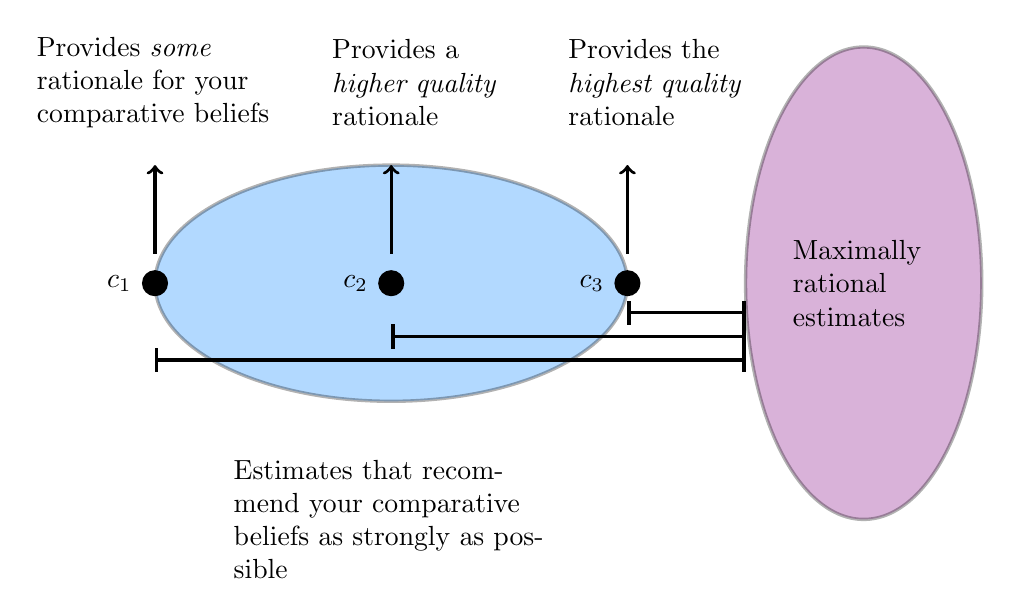
\begin{tikzpicture}[scale = 1.5]
	\draw [very thick, black,fill=blue!50!cyan,opacity=0.3] (0,0) ellipse (2cm and 1cm);
	\draw [very thick, black,fill=blue!50!red,opacity=0.3] (4,0) ellipse (1cm and 2cm);
	
	\node[circle,fill=black!100, minimum size=0.3cm,label=left:{$c_1$}] (n1) at (-2,0) {};
		\node[circle,fill=black!100, minimum size=0.3cm,label=left:{$c_2$}] (n1) at (0,0) {};
		\node[circle,fill=black!100, minimum size=0.3cm,label=left:{$c_3$}] (n1) at (2,0) {};
		
						\draw[very thick,|-|] (2,-.25) -- (3,-.25);
						\draw[very thick,|-|] (0,-.45) -- (3,-.45);
						\draw[very thick,|-|] (-2,-.65) -- (3,-.65);
						\draw[very thick,->] (-2,.25) -- (-2,1);
									\draw[very thick,->] (0,.25) -- (0,1);
										\draw[very thick,->] (2,.25) -- (2,1);

	
	\node[text width=4cm] at (0,-2) {Estimates that recommend your comparative beliefs as strongly as possible};
		\node[text width=1.8cm] at (4,0) {Maximally rational estimates};
		\node[text width=3cm] at (-2,1.7) {Provides \textit{some}\\rationale for your\\comparative beliefs};
				\node[text width=3cm] at (.5,1.7) {Provides a\\\textit{higher quality}\\rationale};
							\node[text width=3cm] at (2.5,1.7) {Provides the\\\textit{highest quality}\\rationale};
\end{tikzpicture}
\caption{More rational estimates provide higher quality rationales.}\label{konek-fig-5}
\end{figure}

The big lingering question is this: when exactly does a set of truth-value estimates \textit{recommend} a certain set of comparative beliefs more or less strongly? There are a number of ways one could spell this out. We will not defend a particular account of recommendation here. But here are three options.
\begin{quote}
\textbf{Metaphysical Account.} The truth-value estimates given by $c:\F\rightarrow\mathbb{R}$ recommend $\succeq$ to degree $k$ iff it is \textit{metaphysically necessary} that any agent who explicitly judges $c(X)$ to be the best truth-value estimate for $X$, for all $X\in\F$, has comparative beliefs $\succeq_c$ and $\D(\succeq_c,\succeq)=1/k$, where $\D$ is some reasonable measure of distance between comparative belief relations. 
\end{quote}
On the metaphysical account, judging $c:\F\rightarrow\mathbb{R}$ to encode the best truth-value estimates for propositions in $\F$ \textit{entails} having certain comparative beliefs $\succeq_c$. Since having comparative beliefs $\succeq_c$ is part and parcel of judging $c$ best, $c$ recommends $\succeq_c$ as strongly as possible. And $c$ recommends other comparative beliefs, $\succeq$, less strongly the further away they are from $\succeq_c$. See \citet{Deza2009} and \citet{Fitelson2015} for more information on measures of distance between comparative belief relations.

Our next account says that while judging $c$ to encode the best truth-value estimates may not \textit{entail} that you have some set of comparative beliefs or other, it nevertheless \textit{rationally requires} you to have those beliefs. And we can use this fact to say what it is for a set of truth-value estimates to \textit{recommend} comparative belief relations to different degrees.
\begin{quote}
\textbf{Normative Account.} The truth-value estimates given by $c:\F\rightarrow\mathbb{R}$ recommend $\succeq$ to degree $k$ iff it is \textit{rationally required} that any agent who explicitly judges $c(X)$ to be the best truth-value estimate for $X$, for all $X\in\F$, has comparative beliefs $\succeq_c$ and $\D(\succeq_c,\succeq)=1/k$, where $\D$ is some reasonable measure of distance between comparative belief relations. 
\end{quote}

A proponent of the normative account might treat the principles of rationality that generate the relevant requirement as properly basic components of her epistemology. Alternatively, she might provide a teleological explanation of why those principles have the normative force that they do by appealing to facts about \textit{epistemic value} or \textit{utility}. One final account of recommendation---the \textit{epistemic utility account}---explains recommendation more directly in terms of epistemic value/utility facts. Informally, the epistemic utility account says that $c$ recommends $\succeq$ to degree $k$ just in case the most rational way of adding estimates of the \textit{value} of comparative beliefs to the stock of truth-value estimates encoded by $c$ involves estimating $\succeq$ to have epistemic utility $k$.

Let's make this a little more precise. An assignment of truth-value estimates $c:\F\rightarrow\mathbb{R}$ (or set $\C$) maps a very specific kind of measurable quantity---\textit{propositions} or \textit{indicator functions}---to estimates. Let $\mathbb{Q}$ be the set of all measurable quantities $\Q:\Omega\rightarrow\mathbb{R}$. An assignment $\est:\mathbb{Q}\rightarrow\mathbb{R}$ of estimates to measurable quantities extends $c$ just in case $c(X)=\est(X)$ for all $X\in\F$.

To make sense of something being closer or further from rational, we need two things: an epistemic utility function $\U$ and laws of preference $\mathcal{L}$.

First let's talk about $\U$. For any assignment of truth-value estimates $c$, $\U(c,w)$ measures how epistemically valuable $c$ is at world $w$. Whatever properties make truth-value estimates epistemically valuable at a world, $\U(c,w)$ captures the extent to which $c$ has a good balance of these properties at $w$. Likewise, $\U(\succeq,w)$ measures how epistemically valuable comparative beliefs $\succeq$ are at world $w$. For a philosophically rich discussion of how to measure the epistemic value of estimates, see \citet{Joyce2009} and \citet{Pettigrew2016}.

Laws of preference $\mathcal{L}$ are familiar from decision theory. In conjunction with $\U$, they specify rationally permissible ways of structuring one's preferences over options. For example, the law of dominance says that if one option $o$ is \textit{guaranteed} to have higher utility than another option $o^*$, then you ought to prefer $o$ to $o^*$. Likewise, the law of (first-order) stochastic dominance says: if for any possible utility value $x$, $o$ is guaranteed to have greater chance than $o^*$ of having higher-than-$x$ utility, then you ought to prefer $o$ to $o^*$. And so on.

Let $\T$ be the set of rational truth-value estimates, relative to $\U$ and $\mathcal{L}$, \textit{i.e.}, the set of $c$ are not dispreferred to some other $c^*$. Let $\E$ be the set of rational estimates more generally relative to $\U$ and $\mathcal{L}$, \textit{i.e.}, the set of $\est$ that are not dispreferred to some other $\est^*$.

Say that $\est$ is the \textit{maximally rational extension} of $c$ to $\mathbb{Q}$ iff (i) $\est$ extends $c$ to $\mathbb{Q}$, and (ii) $\est$ is closer to rational (\textit{i.e.}, closer to $\E$) than any other $\est^*$ that extends $c$ to $\mathbb{Q}$.

We can now state the epistemic utility account more precisely.
\begin{quote}
\textbf{Epistemic Utility Account.} The truth-value estimates given by $c:\F\rightarrow\mathbb{R}$ recommends $\succeq$ to degree $k$ iff the maximally rational extension of $c$ to $\mathbb{Q}$, $\est_c$, is such that such that $\est_c(\U(\succeq))=k$.
\end{quote}
The basic thought here is that while $c$ might not \textit{directly} encode estimates of quantities other than truth-values, it nonetheless takes a stand on how to estimate those quantities. It encodes such estimates \textit{indirectly}. There is some most rational way of adding estimates of other measurable quantities $\Q$ to the stock of truth-value estimates encoded by $c$. These estimates, $\est_c(\Q)$, are the best estimates of those quantities, from $c$'s perspective. So, in effect, the epistemic utility account says that $c$ recommends $\succeq$ to degree $k$ just in case it indirectly estimates $\succeq$ to be epistemically valuable to degree $k$.

There are no doubt myriad unanswered questions about each of these accounts of recommendation. It is not our purpose to provide a full defense of any particular account. Just note that you can choose your favourite (or one not on the list) and slot it into our official version of epistemic interpretivism.
\begin{quote}
\textbf{Epistemic Interpretivism.} A function $c$ (or set $\C$) counts as ``your credal state'' iff it best rationalises your comparative beliefs $\succeq$. Moreover, $c$ (or set $\C$) best rationalises $\succeq$ iff (i) it recommends $\succeq$ as strongly as possible, so that no other $c^*$ (or set $\C^*$) recommends $\succeq$ to a higher degree, and (ii) $c$ is itself closer to rational (closer to $\T$) than any other $c^*$ that recommends $\succeq$ as strongly as possible, and so provides the highest quality recommendation possible. 
\end{quote}

Even setting aside questions about how to understand \textit{recommendation}, there are various lingering questions about epistemic interpretivism. For example, one might wonder what makes comparative beliefs more or less epistemically valuable at a world, or how to measure such value. See \citet{Fitelson2015} for an investigation of ``additive'' epistemic utility measures for comparative belief. One might also wonder what makes one set of estimates closer to rational than another. For a nuanced discussion, see \citet{Staffel2018}. We will not address these questions here. But we will evaluate epistemic interpretivism in a bit more depth in \autoref{konek-sec-7}.


\section{Challenges to the Relevance of Representation Theorems}\label{konek-sec-4}

We now have a number of accounts of credence on the table, however briefly sketched. These accounts purport to tell us what it means to say that an agent is $x\%$ confident in a proposition (if she has precise credences), or between $y\%$ and $z\%$ confident (if she has imprecise credences).

Proponents of these accounts use them to answer some important questions. For example, when exactly \textit{is} there a real-valued function $c$ (or set $\C$) that plays the relevant theoretical role $\R$ well enough to count as ``your credal state''? Following \citet{Meacham2011}, we will call this the \textit{characterisation question}. And why should we expect \textit{rational} agents to have \textit{probabilistically coherent} credences? We will call this the \textit{normative question}.

In answering these questions, proponents typically invoke coherence constraints (on either preference or comparative belief) and representation theorems. \citet{Hajek2009b}, \citet{Meacham2011}, and \citet{Titelbaum2015} challenge any such approach. Whatever account of credence you adopt, they argue, there is no plausible representation-theorem-centric narrative that could answer these questions. Their objections are many. We will focus on a few central ones.

H\'{a}jek, Meacham and Weisberg, and Titelbaum all imagine that the ``basic representation theorem argument'' goes as follows.
\begin{enumerate}
\item[1.] \textit{Coherence Constraints}. Any rational agent's comparative belief relation $\succeq$ satisfies coherence constraints $\phi$. 
\item[2.] \textit{Representation Theorem}. Relation $\succeq$ satisfies constraints $\phi$ if and only if $\succeq$ fully agrees (or almost agrees, or partially agrees, or strongly agrees) with some probability function $c$ (or set of probability functions $\C$).
\item[C.] \textit{Probabilism}. Any rational agent has probabilistic credences (either precise credences given by $c$, or imprecise credences given by $\C$).
\end{enumerate}
If successful, this argument would at least partially answer both the characterisation and normative question at once. When is there a credence function $c$, or a set of such functions $\C$, that plays the relevant theoretical role $\R$ well enough to count as your credal state? Whenever your comparative beliefs satisfy coherence constraints $\phi$! Satisfying $\phi$ is a sufficient condition for having credences. And why should we expect \textit{rational} agents to have \textit{probabilistically coherent} credences? Because the coherence constraints $\phi$ are rationally mandatory. And any agent who satisfies $\phi$ not only has credences, but \textit{probabilistically coherent} credences.

But this argument is \textit{not} successful as it stands. As \citet{Eriksson2007}, \citet{Hajek2009b}, \citet{Meacham2011}, and \citet{Titelbaum2015} emphasise, it does not follow from the mere fact that some probabilistically coherent credence function \textit{fully agrees} with her comparative beliefs that she in fact \textit{has} probabilistic credences. So the argument is invalid. H\'{a}jek puts the point as follows (\textit{cf.} also \citealp[p. 14]{Meacham2011}, and \citealp[p. 274]{Titelbaum2015}):
\begin{quote}
the mere \emph{possibility} of representing you one way or another might have less force than we want; your acting \emph{as if} the representation is true of you does not make it true of you. To make this concern vivid, suppose that I represent your preferences with \emph{Voodooism}. My voodoo theory says that there are warring voodoo spirits inside you. When you prefer $A$ to $B$, then there are more $A$-favouring spirits inside you than $B$-favouring spirits [\ldots] I then `prove' Voodooism: if your preferences obey the usual rationality axioms, then there exists a Voodoo representation of you. That is, you act \emph{as if} there are warring voodoo spirits inside you in conformity with Voodooism. Conclusion: rationality requires you to have warring Voodoo spirits in you. Not a happy result. \citep[p. 238]{Hajek2009b}
\end{quote}
The same thing, these objectors claim, can be said about the representation theorem argument for probabilism. Just because your preferences can be \emph{represented} as the end product of a vigorous war between the voodoo spirits inside you does not imply that you \emph{in fact} have such spirits inside you. Similarly, just because your comparative beliefs can be \emph{represented} as arising from precise credences $c$ (or imprecise credences $\C$) does not imply that you \emph{in fact} have such credences.

This line of criticism is not particularly concerning. The reason: no Bayesians put forward this basic ``representation theorem argument.'' \citeauthor{Koopman1940b}, \citeauthor{Savage1954}, \citeauthor{Joyce2010}, etc.; they all presuppose \textit{some} account of credence or other. For example, \citeauthor{Krantz1971} presuppose a measurement-theoretic account of credence. 
\begin{quote}
we inquire into conditions under which an ordering $\succeq$ of $\mathscr{E}$ has an order-preserving function $P$ that satisfies Definition 2. Obviously, the ordering is to be interpreted empirically as meaning ``qualitatively at least as probable as.'' Put another way, we shall attempt to treat the assignment of probabilities to events as a measurement problem of the same fundamental character as the measurement of, e.g., mass or momentum. \citep[pp. 199--202]{Krantz1971} 
\end{quote}
The upshot: any faithful reconstruction of the ``representation theorem argument'' really ought to feature an account of credence explicitly as a premise. The simple argument under attack here fails this basic test.

Of course, objectors do not focus exclusively on this simple version of the representation theorem argument. H\'{a}jek, Meacham and Weisberg, and Titelbaum all consider more sophisticated versions as well. A fairly general, more charitable way of understanding what fans of representation theorems are up to is this. Firstly, to shed some light on the characterisation question, they establish a ``Bridge Theorem'' which shows that the function $c$, or set of functions $\C$, outputted by their favourite representation theorem is fit to play the theoretical role $\R$ singled out by their favourite account of credence.
\begin{quote}
\textbf{Bridge Theorem.} If $\succeq$ satisfies $\phi$, then at least one of the probability functions $c$ (or set of probability functions $\C$) whose existence is guaranteed by the \textit{Representation Theorem} plays role $\R$ well enough to count as ``your credal state.''
\end{quote}
Secondly, to answer the normative question, they put their favourite account of credence, their favourite representation theorem, and this bridge theorem to work in order to provide a more sophisticated argument for probabilism.
\begin{enumerate}
\item[1.] \textit{Coherence Constraints}. Any rational agent's comparative belief relation $\succeq$ satisfies coherence constraints $\phi$. 
\item[2.] \textit{Theory of Credence}. A real-valued function $c$ (or set $\C$) counts as ``your credal state'' to the extent that it plays theoretical role $\R$. The better $c$ (or $\C$) plays role $\R$, the more eligible it is as a ``credal state candidate.''
\item[3.] \textit{Representation Theorem}. Relation $\succeq$ satisfies constraints $\phi$ if and only if $\succeq$ fully agrees (or almost agrees, or partially agrees, or strongly agrees) with some probability function $c$ (or set of probability functions $\C$).
\item[4.] \textit{Bridge Theorem}. If $\succeq$ satisfies $\phi$, then at least one of the probability functions $c$ (or set of probability functions $\C$) whose existence is guaranteed by the \textit{Representation Theorem} plays role $\R$ well enough to count as ``your credal state.''
\item[C.] \textit{Probabilism}. Any rational agent has probabilistic credences (either precise credences given by $c$, or imprecise credences given by $\C$).
\end{enumerate}
In \autoref{konek-sec-5}--\ref{konek-sec-7}, we will evaluate how this argument fares on each of our competing accounts of credence. But it is worth addressing some \textit{general} concerns about this argumentative strategy here.\footnote{The following objections are adapted from \citet{Hajek2009b}, \citet{Meacham2011}, and \citet{Titelbaum2015}.}

Meacham and Weisberg worry that even if the axioms $\phi$ of your favourite representation theorem encode genuine coherence constraints on \textit{rational} comparative belief, ordinary folks like you and me are not typically rational \citep[pp. 7--8]{Meacham2011}.\footnote{Meacham and Weisberg are concerned primarily with representation theorems for \textit{preference relations}. Accordingly, they focus on empirical data that shows that ordinary agents reliably violate putative coherence constraints on rational preference. For example, \citet{Kahneman1979} show that subjects consistently violate Savage's Independence Axiom, and \citet{Lichtenstein1971, Lichtenstein1973} show that subjects often have intransitive preferences. We adapt their concerns to the case of comparative belief \textit{mutatis mutandis}.} Our comparative beliefs violate these constraints $\phi$. So even if the Bridge Theorem is correct---even if the representation theorem in question \textit{would} output a function $c$, or a set of functions $\C$ that deserves to be called ``your credal state'' \textit{if} your comparative beliefs satisfied $\phi$---it is silent about ordinary folks. The upshot: it does not help to answer the characterisation question in any interesting way. While it does specify sufficient conditions for having credences, those conditions are so demanding that they are more or less irrelevant for agents like us.

This concern, however, does not cut much ice. As we will see in \autoref{konek-sec-5}--\ref{konek-sec-7}, there is plenty to say about when ordinary folks---folks who reliably violate constraints of rationality---count as having credences on each of our competing accounts (measurement-theoretic, decision-theoretic, and epistemic interpretivist).

Meacham and Weisberg also worry that the ``representation theorem argument'' trivialises normative epistemology \citep[pp. 14--16]{Meacham2011}. There is a gap, recall, between representability and psychological reality. Just because your comparative beliefs can be \emph{represented} as arising from precise credences $c$ (or imprecise credences $\C$) does not imply that you \emph{in fact} have such credences. To avoid this problem, the objection goes, representation theorem arguments must \textit{stipulatively define} an agent's credences to be given by the function $c$ (or set $\C$) outputted by one's favourite representation theorem. But those theorems deliver probabilistic representations by construction. So it is simply true \textit{by stipulative definition} that whenever an agent has credences, they are probabilistically coherent. Whence the normative force of probabilism then? The claim that \textit{rational} credences are probabilistically coherent is trivial if \textit{all} credences are probabilistically coherent \textit{by definition}.

But again this concern need not give us much pause. We do \textit{not} need to bridge the gap between representability and psychological reality by stipulative definition. Rather, we bridge that gap by (i) providing a theory of credence, which specifies the theoretical role $\R$ that a function $c$ (or set $\C$) must play to count as ``your credal state,'' and (ii) providing a bridge theorem, which establishes that some function $c$ (or set $\C$) outputted by one's favourite representation theorem in fact plays role $\R$ sufficiently well. This strategy does \textit{not} stipulatively define your credences as those given by $c$ (or $\C$). Far from it. Establishing that $c$ (or $\C$) plays $\R$ well enough to count as ``your credal state'' requires \textit{substantive argumentation}.

It is safe, then, to put these general concerns to the side. Of course, their spectre lingers until we see the details about the relevant bridge theorems and so on (\autoref{konek-sec-5}--\ref{konek-sec-7}). We now turn our attention to evaluating how well this strategy answers the characterisation and normative questions, respectively, on each of our competing accounts of credence.



\section{Evaluating the Measurement-Theoretic View}\label{konek-sec-5}


\subsection{Interpreting Credence Functions}

On the measurement-theoretic view, a credence function $c$ (or set $\C$) is a mere numerical measurement system. It allows you to represent an agent's comparative belief structure, $\left<\Omega,\F,\succeq\right>$, numerically in the following sense. Firstly, $c$ maps the propositions $X$ in $\F$ to real-valued proxies, $c(X)$. Secondly, it does so in a ``structure-preserving fashion.'' If $c$ fully agrees with $\succeq$, then one proxy $c(X)$ is larger than another $c(Y)$ exactly when our agent is more confident in $X$ than $Y$ (and $c(X)=c(Y)$ exactly when she is equally confident in $X$ and $Y$): 
$$ X\succeq Y \Leftrightarrow c(X)\geq c(Y). $$
In this sense, the familiar ``greater than or equal to'' relation $\geq$ on the real numbers ``preserves the structure'' of our agent's comparative belief relation $\succeq$ on $\F$. Because of this, you can use the numerical measurement system in helpful ways. You can elicit certain comparative beliefs, infer properties of $c$, perform numerical calculations, and draw conclusions about what other comparative beliefs she must have (or must not have).

Similarly, a \textit{set} of real-valued functions $\C$ can provide a numerical measurement system for $\succeq$. If $\C$ fully agrees with $\succeq$, then the $c$ in $\C$ uniformly assign larger proxies to $X$ than $Y$ exactly when our agent is more confident in $X$ than $Y$ (and uniformly assign equal proxies exactly when she is equally confident in $X$ and $Y$): 
$$ X\succeq Y \Leftrightarrow c(X) \geq c(Y) \text{ for all } c\in\C. $$
Once more, this allows you to \textit{use} the (imprecise) numerical measurement system $\C$ in helpful ways. You can elicit certain comparative beliefs, infer properties of $\C$, perform numerical calculations, and draw conclusions about what other comparative beliefs she must have (or must not have).

Weaker types of agreement yield numerical measurement systems fit for slightly different purposes. Suppose, for example, that $c$ \textit{strongly agrees} with $\succeq$:
$$
\begin{aligned}
	X\succeq Y &\Rightarrow c(X)\geq c(Y),\\
	X \succ Y  &\Rightarrow c(X)>c(Y).
\end{aligned}
$$
Such a measurement system licenses fewer inferences about $\succeq$ than fully agreeing systems. To see this, imagine that $c$ is a probability function, $X$ and $Y$ are both incompatible with $Z$, and $X\succ Y$. Then since $c$ strongly agrees with $\succeq$, we have $c(X)>c(Y)$. And since $c$ is a probability function, $c(X\cup Z)>c(Y\cup Z)$. Hence $c(X\cup Z)\not\leq c(Y\cup Z)$. From this we can infer that $X\cup Z \not\preceq Y\cup Z$. But we \textit{cannot} infer that $X\cup Z \succeq Y\cup Z$. If, on the other hand, $c$ were to \textit{fully} agree with $\succeq$, then we \textit{could} make this latter inference.

To recap: the measurement-theoretic view takes a particular stand on the nature of the theoretical role $\R$ that a function $c$ (or set $\C$) must play in order to count as ``your credal state.'' More specifically, $c$ (or $\C$) must fully agree (or almost agree, or partially agree, or strongly agree) with the agent's comparative beliefs, $\succeq$, in the way required to count as a numerical measurement system for $\succeq$. The better $c$ (or $\C$) plays this role $\R$, the more eligible it is as a credal state candidate.

Importantly, though, \textit{any} function $c$ (or set $\C$) that plays this role $\R$ has equal claim to be called ``your credence function,'' on the measurement-theoretic view. \emph{Any} order-preserving mapping (homomorphism) from $\F$ into $\mathbb{R}$ is just as eligible as a credal state candidate as any other. So credence functions are not unique. Indeed, if $c$ fully agrees (or almost agrees, or partially agrees, or strongly agrees) with $\succeq$, then any of the infinitely many strictly increasing transformations of $c$ do so as well. So if you have \emph{one} credence function, on this view, then you have \emph{infinitely many}.

In addition, \textit{interpreting} credence functions requires care, on the measurement-theoretic view. An agent's credence function does not wear its representationally significant features on its sleeve. Sorting out which features of one's credence function are representationally significant, rather than ``mere artefacts,'' requires knowing what the ``permissible transformations'' of that credence function are. That is, it requires knowing not only that $b$ counts as ``your credence function,'' but also what \textit{other} functions $c$ preserve the structure of your comparative and qualitative beliefs, and so count as ``your credence function'' as well. For example, on the standard Bayesian picture, an agent's credence function $c$ is such that
\[
\frac{c(X\cap Y)}{c(Y)} = c(X)
\]
just in case she judges that $Y$ is evidentially independent of $X$. But if credence functions $c$ are mere numerical measurement systems for an agent's comparative beliefs $\succeq$, then properties like $c(X\cap Y)/c(X)=c(Y)$ are \textit{not} representationally significant. They do not reflect anything \textit{real} about the agent's doxastic state.

To see this, imagine that you take two blood tests. Let $w^+_+$ be the world in which both tests come back positive; $w^+_-$ be the world in which the first comes back positive and the second negative; $w^-_+$ be the world in which the first comes back negative and the second positive; and $w^-_-$ be the world in which both tests come back negative. You have comparative beliefs over propositions in the following Boolean algebra:
$$
\F=\left\{
\begin{tabular}{c}
  $\left\{w^+_+,w^+_-,w^-_+,w^-_-\right\}$ \\
  $\left\{w^+_+,w^+_-,w^-_+\right\}, \left\{w^+_+,w^+_-,w^-_-\right\}$\\
  $\left\{w^+_+,w^-_+,w^-_-\right\}, \left\{w^+_-,w^-_+,w^-_-\right\}$ \\
  $\left\{w^+_+,w^+_-\right\}, \left\{w^+_+,w^-_+\right\}, \left\{w^+_+,w^-_-\right\}$\\
  $\left\{w^+_-,w^-_+\right\}, \left\{w^+_-,w^-_-\right\}, \left\{w^-_+,w^-_-\right\}$,\\
  $\left\{w^+_+\right\}, \left\{w^+_-\right\}, \left\{w^-_+\right\},\left\{w^-_-\right\}$,\\
  $\varnothing$ \\
\end{tabular}
\right\}.
$$
In particular, your comparative beliefs are given by:
\begin{gather*}
\left\{w^+_+,w^+_-,w^-_+,w^-_-\right\}\succ\left\{w^+_+,w^-_+,w^-_-\right\}\succ\left\{w^+_+,w^+_-\right\}\\
\succ\left\{w^-_+,w^+_-,w^-_-\right\}\succ\left\{w^+_-,w^-_-\right\}\succ\left\{w^-_+,w^+_-\right\}\succ\left\{w^+_-\right\}\\
\succ\left\{w^+_+,w^-_+,w^-_-\right\}\succ\left\{w^+_+,w^-_-\right\}\succ\left\{w^+_+,w^-_+\right\}\succ\left\{w^+_+\right\}\\
\succ\left\{w^-_+,w^-_-\right\}\succ\left\{w^-_-\right\}\succ\left\{w^-_+\right\}\succ\varnothing.
\end{gather*}
Then the probability functions $b$ and $c$ in \autoref{konek-table-1} both fully agree with $\succeq$, and hence both count as a numerical measurement systems for $\succeq$. 
\begin{table}[ht]
\centering
\def\arraystretch{1.25}
\begin{tabular}{ccccc}
\hline
& $w^+_+$&$w^+_-$&$w^-_+$&$w^-_-$\\
\hline\hline
$b$ & $\frac{11}{36}$ & $\frac{22}{36}$ & $\frac{1}{36}$ & $\frac{2}{36}$\\
$c$ & $\frac{20}{64}$ & $\frac{33}{64}$ & $\frac{4}{64}$ & $\frac{7}{64}$\\
\hline
\end{tabular}
\caption{Probability functions $b$ and $c$ on $\F$. Both fully agree with $\succeq$.}\label{konek-table-1}
\end{table}
So both play the credal state role, on the measurement-theoretic view. But $b$ is such that
$$ \frac{b(\left\{w^+_+\right\})}{b(\left\{w^+_+,w^+_-\right\})}=\frac{1}{3} = b(\left\{w^+_+,w^-_+\right\}). $$
Given that $b$ is your credence function, the standard interpretation says: you think that the result of the first test provides no evidence one way or the other about the result of the second test. On the other hand, $c$ is such that
$$ \frac{c(\left\{w^+_+\right\})}{c(\left\{w^+_+,w^+_-\right\})}=\frac{20}{53}>\frac{24}{64} = c(\left\{w^+_+,w^-_+\right\}). $$
Given that $c$ is your credence function, the standard interpretation says: you judge that a positive outcome on the second test \textit{supports} or \textit{confirms} a positive outcome on the first test. Finding out that the second test is positive \textit{increases} your credence that the first test is positive too.

What is going on here? Answer: the ``standard interpretation'' reads more information into one's credence function than is actually encoded in that credence function. On the measurement-theoretic view, credence functions are nothing more than numerical measurement systems that encode the ordering determined by your comparative beliefs. (They are mere ``ordinal scale'' measurement systems, not ``ratio scale'' measurement systems.) But there is more to making judgments of evidential relevance and irrelevance than having a particular constellation of comparative beliefs. Agents who only have comparative beliefs simply are not opinionated enough to count as having opinions about evidential relevance and irrelevance. So credence functions do not reflect any such opinions.

Interpreting \textit{imprecise} credal states requires care too. Suppose, for example, that you have opinions about the propositions in the Boolean algebra
$$ \F^*=\left\{\Omega, X, \neg X,\varnothing\right\}. $$
Consider the precise and imprecise credal states on $\F^*$ given by the probability function $b$ in \autoref{konek-table-2}
\begin{table}[ht]
\centering
\begin{tabular}{ccccc}
\hline
& $\Omega$&$X$&$\neg X$&$\varnothing$\\
\hline\hline
$b$ & $1$ & $0.7$ & $0.3$ & $0$\\
\hline
\end{tabular}
\caption{Probability function $b$ on $\F^*$}\label{konek-table-2}
\end{table}
and the set of probability functions $\C$:
$$ \C=\left\{c \mathrel{|} c(\Omega)>c(X)>c(\neg X)>c(\varnothing)\right\}. $$
On the standard interpretation, $b$ and $\C$ represent different doxastic states. An agent with credence function $b$ is precisely $70\%$ confident that $X$ is true. An agent with imprecise credal state $\C$, in contrast, is at least $50\%$ confident that $X$ is true, but nothing stronger. On the standard interpretation, these are not idle differences. These differences in doxastic states are reflected in one's evaluative attitudes. For example, an agent with credence function $b$ will have precisely the same fair buying and selling price for a unit gamble $\G$ on $X$, \textit{viz.}, $0.7$. Paying any price up to \textsterling$0.7$ for $\G$ is a good deal in her view. Selling $\G$ for any price over \textsterling$0.7$ is a good deal. But an agent with imprecise credal state $\C$ will have different buying and selling prices for $\G$. Paying any price up to \textsterling$0.5$ for $\G$ is a good deal, in her view. But selling $\G$ is only a determinately good deal if the buyer is willing to pay more than \textsterling$1$.

On the measurement-theoretic view, however, $b$ and $\C$ represent \textit{exactly the same doxastic state}. They both fully agree with the following comparative belief relation $\succeq$:
$$ \Omega\succ X\succ \neg X\succ\varnothing. $$
They are both order-preserving mappings from $\F^*$ into the reals \textit{that preserve exactly the same structure}. In this case, there is simply no substantive difference between being $70\%$ confident, or $89.637\%$ confident, or at least $50\%$ confident that $X$ is true. Only the comparative beliefs that $b$ and $\C$ encode are psychologically real. Everything else is a ``mere artefact'' of one's preferred numerical measurement system. Both $b$ and $\C$, and any other credal state that fully agrees with $\succeq$, plays exactly the same theoretical role: they represent the comparative beliefs captured by $\succeq$ in an elegant, easy-to-use, numerical fashion---nothing more, nothing less.


\subsection{Unary and Pluralist Variants}

We have focussed thus far on a particular \textit{unary} variant of the measurement-theoretic view. On this view, credence functions are mere numerical measures of one's \textit{comparative beliefs}. Having credences is nothing over and above having numerically representable comparative beliefs. You might be attracted to this view if, for example, you think that we can explain and rationalise everything important about choice and inference by appealing exclusively to comparative belief---no additional modes or types of doxastic judgment necessary. In that case, you might say: to the extent that we are willing to talk about \textit{prima facie} distinct types of opinion---degrees of belief, full or categorical belief, etc.---they ought to ultimately reduce to comparative beliefs. Reducing those other types of opinion away will allow us to provide the simplest and most unified possible explanations of the relevant data regarding choice and inference.

But there is also a \textit{pluralist} variant of the measurement-theoretic view, which you might find attractive if you are less optimistic about the explanatory power of comparative belief. On the pluralist version, agents have a genuine plurality of doxastic attitudes, not simply comparative beliefs. In addition to comparative beliefs, agents also have: (i) opinions about the \emph{evidential dependence or independence} of one hypothesis on another; (ii) opinions about the \emph{causal dependence or independence} of one variable on another; (iii) \emph{full} or \textit{categorical beliefs}; they may even (iv) explicitly \emph{estimate} the values of all sorts of different variables, including the frequency of truths in a set of propositions, and the truth-values of individual propositions. Estimating, in this sense, is a matter of making a \emph{sui generis} doxastic judgment---a type of judgment that may bear interesting relations to other types of judgments (normative relations, causal relations, etc.), but is not reducible to them. Estimating the truth-value of a proposition, in this sense, is what \citet{Jeffrey2002} calls having an \emph{exact judgmental probability} for the truth of that proposition.

On the pluralist measurement-theoretic view, your credence function \textit{is} a mere numerical measurement system, but not a measure specifically \emph{of your comparative belief relation}. Rather, on the pluralist view, you have a genuine plurality of comparative and qualitative doxastic attitudes, and your credence function is a measure of that \emph{entire system of attitudes}.

Consider once again our blood test example. You have the following comparative beliefs:
\begin{gather*}
\left\{w^+_+,w^+_-,w^-_+,w^-_-\right\}\succ\left\{w^+_+,w^+_-,w^-_-\right\}\succ\left\{w^+_+,w^-_+,w^+_-\right\}\\
\succ\left\{w^+_+,w^+_-\right\}\succ\left\{w^-_+,w^+_-,w^-_-\right\}\succ\left\{w^+_-,w^-_-\right\}\succ\left\{w^-_+,w^+_-\right\}\\
\succ\left\{w^+_-\right\}\succ\left\{w^+_+,w^-_+,w^-_-\right\}\succ\left\{w^+_+,w^-_-\right\}\succ\left\{w^+_+,w^-_+\right\}\\
\succ\left\{w^+_+\right\}\succ\left\{w^-_+,w^-_-\right\}\succ\left\{w^-_-\right\}\succ\left\{w^-_+\right\}\succ\varnothing.
\end{gather*}
But now imagine that you have a wide range of comparative and qualitative opinions, not just comparative beliefs. You think, for example, that when you find out the result of the first test (positive or negative), this provides no evidence one way or the other about the result of the second test. (Perhaps the tests probe two different, unrelated conditions.) That is, you judge $\{w^+_+,w^+_-\}$ and $\{w^-_+,w^-_-\}$ to be \emph{evidentially independent} of $\{w^+_+,w^-_+\}$ and $\{w^+_-,w^-_-\}$, and vice versa.

In addition, you have certain \emph{full beliefs} or \emph{categorical beliefs}. Let's suppose that you believe that the first test will come back positive. (It probes for a condition that you quite clearly have.) That is, you fully believe $\{w^+_+,w^+_-\}$. And you believe all of the logical consequences of this proposition. But you have no further full or categorical beliefs.

Finally, you judge $1/3$ to be the \emph{best estimate} of the truth-value of the proposition that the second test will come back positive. (Recall, a proposition's truth-value is $1$ if it is true and $0$ if it is false.) In Jeffrey's parlance, you have a judgmental probability of $1/3$ for the proposition $\{w^+_+,w^-_+\}$.

So you have a genuine plurality of doxastic attitudes: you have comparative beliefs; you make evidential independence judgments; you have full or categorical beliefs; you also estimate the truth-values of certain propositions (you have exact judgmental probabilities). On the pluralist measurement-theoretic view, your credence function is a measure of this entire system of attitudes.

To make this more precise, let's model your doxastic attitudes using a relational structure:
$$ \A=\left<\F,\succeq,\I,\B,\E_{1/3}\right>. $$
$\A$ comprises your Boolean algebra $\F$ of subsets of $\Omega=\{w^+_+,w^+_-,w^-_+,w^-_-\}$, together with a \textit{comparative belief relation} $\succeq$ on $\F$, an \textit{independence relation} $\I$, a (unary) \textit{belief relation} $\B$, and a (unary) \textit{estimation relation} $\E_{1/3}$. 


$\I$ models your evidential independence judgments. It will be convenient to think of $\I$ as a $3$-place relation on $\F$:
\begin{quote}\centering
$\I(X,Y,X\cap Y)$\\
\textit{iff}\\
you judge $X$ to be evidentially independent of $Y$.
\end{quote}
Since you judge $\{w^+_+,w^+_-\}$ and $\{w^-_+,w^-_-\}$ to be independent of $\{w^+_+,w^-_+\}$ and $\{w^+_-,w^-_-\}$, and vice versa, we have:
$$
\begin{aligned}
	\I(\left\{w^+_+,w^+_-\right\},\left\{w^+_+,w^-_+\right\},\left\{w^+_+\right\}),\\
	\I(\left\{w^-_+,w^-_-\right\},\left\{w^+_+,w^-_+\right\},\left\{w^-_+\right\}),\\
	\I(\left\{w^+_+,w^+_-\right\},\left\{w^+_-,w^-_-\right\},\left\{w^+_-\right\}),\\
	\I(\left\{w^-_+,w^-_-\right\},\left\{w^+_-,w^-_-\right\},\left\{w^-_-\right\}).
\end{aligned}
$$
We also have $\I(Y,X,X\cap Y)$ for each of these four independence judgments $\I(X,Y,X\cap Y)$.

Likewise, $\B$ models your full or categorical beliefs:
\begin{quote}\centering
$\B(X)$ \hspace{.3em}\textit{iff}\hspace{.2em} you believe $X$.
\end{quote}
Since you believe $\{w^+_+,w^+_-\}$ and all of its logical consequences, we have:
\begin{gather*}
	\B(\left\{w^+_+,w^+_-,w^-_+,w^-_-\right\}),\\
	\B(\left\{w^+_+,w^+_-,w^-_+\right\}),\\
	\B(\left\{w^+_+,w^+_-,w^-_-\right\}),\\
	\B(\left\{w^+_+,w^+_-\right\}).
\end{gather*}

Finally, $\E_{1/3}$ models your explicit estimates of truth-values:
\begin{quote}
{\centering
$\E_{x}(X)$\\
\textit{iff}\\}
you judge $x$ to be the best estimate of the truth-value of $X$.
\end{quote}
Since you judge $1/3$ to be the best estimate of the truth-value of $\{w^+_+,w^-_+\}$, we have:
$$ \E_{1/3}\left(\left\{w^+_+,w^-_+\right\}\right). $$

On the pluralist view, your credence function is a measure of your entire system of attitudes:
$$ \A=\left<\F,\succeq,\I,\B,\E_{1/3}\right>. $$
It is a homomorphism---a structure-preserving mapping---that takes $\A$ into some numerical structure $\A^*$. 
$$ \A^*=\left<\mathbb{R},\succeq^*,\I^*,\B^*,\E_{1/3}^*\right>. $$
That is, your credence function $c$ maps $\F$ into $\mathbb{R}$ in a way that preserves $\A$'s structure, so that:\footnote{We could swap full agreement for almost, or partial, or strong agreement here. Weaker notions of agreement would provide us with weaker notions of structure-preservation.}
\begin{eqnarray*}
X\succeq Y & \Leftrightarrow & c(X)\succeq^* c(Y),\\
\I(X,Y,X\cap Y) & \Leftrightarrow & \I^*(c(X),c(Y),c(X\cap Y)),\\
\B(X) & \Leftrightarrow & \B^*(c(X)),\\
\E_{1/3}(X) & \Leftrightarrow & \E_{1/3}^*(c(X)).
\end{eqnarray*}
\textit{Which} numerical structure $c$ takes $\A$ into, on the measurement-theoretic view, is either a matter of convention or a matter to be decided on practical grounds. For illustrative purposes, let's choose a familiar numerical structure. Let $\succeq^*$ by the ``greater than or equal to'' relation, $\geq$. Let $\I^*$ be the standard probabilistic independence relation:
\begin{quote}\centering
$\I^*(c(X),c(Y),c(X\cap Y))$ \hspace{.3em}\textit{iff}\hspace{.2em} $c(X)c(Y)=c(X\cap Y)$.
\end{quote}
Let $\B^*$ be a \emph{Lockean belief relation}, so that believed propositions $X$ have real-valued proxies $c(X)$ that are greater than (or equal to) some threshold $\tau$ (for concreteness let $\tau=5/6$):
$$ \B^*(c(X)) \textit{ iff } c(X)\geq\tau. $$
Finally, let $\E^*_{1/3}$ be:
$$ \E_{1/3}^*(c(X) \textit{ iff } c(X)=1/3. $$
This ensures that for any structure-preserving measurement system, $c$, you explicitly judge $1/3$ to be the best estimate of $X$'s truth-value just in case $c(X)=1/3$.

The important observation to make is this: the pluralist view carves out a bigger job for credence functions to do than the reductive view. Credence functions must do more than preserve the order induced on $\F$ by your comparative belief relation. They must also preserve the structure induced by your various other doxastic attitudes: your evidential independence judgments, full or categorical beliefs, and so on. So a function $c:\F\rightarrow\mathbb{R}$ may well do the work required to count as ``your credence function'' on the unary view, but yet fall short of that mark on the pluralist view.

Consider, for example, the function $b:\F\rightarrow\mathbb{R}$:
$$
\begin{aligned}
	b(\left\{w^+_+,w^+_-,w^-_+,w^-_-\right\})&=1,& b(\left\{w^+_+,w^-_+,w^-_-\right\})&=31/64,\\
	b(\left\{w^+_+,w^+_-,w^-_-\right\})&=60/64,& b(\left\{w^+_+,w^-_-\right\})&=27/64 ,\\
	b(\left\{w^+_+,w^-_+,w^+_-\right\})&=57/64,& b(\left\{w^+_+,w^-_+\right\})&=24/64,\\
	b(\left\{w^+_+,w^+_-\right\})&=53/64,& b(\left\{w^+_+\right\})&=20/64,\\
	b(\left\{w^-_+,w^+_-,w^-_-\right\})&=44/64,& b(\left\{w^-_+,w^-_-\right\})&=11/64,\\
	b(\left\{w^+_-,w^-_-\right\})&=40/64,& b(\left\{w^-_-\right\})&=7/64,\\ 
	b(\left\{w^-_+,w^+_-\right\})&=37/64,& b(\left\{w^-_+\right\})&=4/64,\\
	b(\left\{w^+_-\right\})&=33/64,& b(\varnothing)&=0.
\end{aligned}
$$
It is easy to verify that $b$ fully agrees with $\succeq$, \textit{i.e.},
$$ X\succeq Y  \Leftrightarrow  b(X)\geq b(Y). $$
So $b$ is a real-valued measure of your comparative belief relation $\succeq$. Hence, it counts as a credence function on the unary measurement-theoretic view. It preserves the structure on $\F$ induced by your comparative beliefs---the only type of doxastic attitude that the unary view countenances. But it does \emph{not} play the theoretical role required to count as a credence function on the pluralist measurement-theoretic view. To do \emph{that}, it must also preserve the structure on $\F$ induced by your various other doxastic attitudes: your independence judgments, full or categorical beliefs, and so on. But $b$ falls short of that mark.

For example, you think that the outcome of the first test provides no evidence about the outcome of the second. But $b$ does not treat $\{w^+_+,w^+_-\}$ and $\{w^+_+,w^-_+\}$, for example, as independent, in the way specified by $\I^*$:
\begin{multline*}
b\left(\left\{w^+_+,w^+_-\right\}\right) b\left(\left\{w^+_+,w^-_+\right\}\right) = \
\frac{53}{64}\cdot\frac{24}{64} = \frac{159}{512} \\
\not = \frac{160}{512} = \frac{20}{64} = \
b\left(\left\{w^+_+\right\}\right).
\end{multline*}
Similarly, you believe that the first test will come back positive. That is, you fully believe $\{w^+_+,w^+_-\}$. But $b$ does not treat $\{w^+_+,w^+_-\}$ as believed, in the way specified by the Lockean belief relation $\B^*$. It maps $\{w^+_+,w^+_-\}$ to a real-valued proxy $b(\{w^+_+,w^+_-\})=53/64\approx 0.828$ below the threshold $\tau=5/6\approx0.833$ required for full or categorical belief.

Finally, you judge $1/3$ to be the best estimate of the truth-value of the proposition that the second test will come back positive. You have a judgmental probability of $1/3$ for the proposition $\{w^+_+,w^-_+\}$. But $b$ fails to map $\{w^+_+,w^-_+\}$ to the real-valued proxy set aside by $\E^*_{1/3}$ for such propositions, \textit{viz.}, $1/3$. Instead, $b(\{w^+_+,w^-_+\})=24/64=0.375$.

The upshot: while $b$ preserves the structure on $\F$ induced by your comparative beliefs, it fails to preserve the additional structure induced by your various other doxastic attitudes: your evidential independence judgments, full or categorical beliefs, and so on. So while $b$ \emph{does} count as one of your (infinitely many) credence functions on the unary measurement-theoretic view, it does \emph{not} count as one on the pluralist measurement-theoretic view.

In contrast, the function $c:\F\rightarrow\mathbb{R}$ of \autoref{konek-fig-4} counts as ``your credence function'' on both the unary and pluralist views. (The interested reader may verify this for herself.)
\begin{figure}[ht]
$$
\begin{aligned}
c(\left\{w^+_+,w^+_-,w^-_+,w^-_-\right\})&=1, & c(\left\{w^+_+,w^-_+,w^-_-\right\})&=\frac{14}{36},\\
c(\left\{w^+_+,w^+_-,w^-_-\right\})&=\frac{35}{36}, & c(\left\{w^+_+,w^-_-\right\})&=\frac{13}{36},\\
c(\left\{w^+_+,w^-_+,w^+_-\right\})&=\frac{34}{36}, & c(\left\{w^+_+,w^-_+\right\})&=\frac{12}{36},\\
c(\left\{w^+_+,w^+_-\right\})&=\frac{33}{36}, & c(\left\{w^+_+\right\})&=\frac{11}{36},\\
c(\left\{w^-_+,w^+_-,w^-_-\right\})&=\frac{25}{36}, & c(\left\{w^-_+,w^-_-\right\})&=\frac{3}{36},\\
c(\left\{w^+_-,w^-_-\right\})&=\frac{24}{36}, & c(\left\{w^-_-\right\})&=\frac{2}{36},\\
c(\left\{w^-_+,w^+_-\right\})&=\frac{23}{36}, & c(\left\{w^-_+\right\})&=\frac{1}{36},\\
c(\left\{w^+_-\right\})&=\frac{22}{36}, & c(\varnothing)&=0.
\end{aligned}
$$
\caption{Credence function $c$}\label{konek-fig-4}
\end{figure}

To recap: the measurement-theoretic view stakes out a particular position on the theoretical role $\R$ that a function $c$ (or set of functions $\C$) must play in order to count as ``your credal state.'' It says that $c$ (or $\C$) must fully agree (or almost agree, or partially agree, or strongly agree) with your comparative and qualitative opinions---comparative beliefs, evidential independence judgments, full or categorical beliefs, etc.---in the way required to count as a numerical measure of that \emph{entire system of attitudes}. The better $c$ (or $\C$) plays this role $\R$, the more eligible it is as a credal state candidate. On the unary measurement-theoretic view, the fundamental type of doxastic attitude is \textit{comparative belief}. So credal states are numerical measures of comparative beliefs. On the pluralist measurement-theoretic view, you have a genuine plurality of doxastic attitudes. So credal states are numerical measures of a more highly structured system of attitudes.

To streamline our discussion, we will focus on the the unary variant of the measurement-theoretic view going forward.










\subsection{The Characterisation and Normative Questions}

How does the unary measurement-theoretic account answer the characterisation question? When exactly \textit{is} there a function $c$ (or set $\C$) that fully agrees (or almost agrees, or partially agrees, or strongly agrees) with your comparative belief relation $\succeq$ in the way required to count as a numerical measure of $\succeq$?


We explored a partial answer to this question earlier. \citet{Scott1964} proves that there is a \textit{probability function} that \textit{fully agrees} with your comparative belief relation $\succeq$ just in case $\succeq$ satisfies Non-Triviality, Non-Negativity, Totality, and Isovalence. \citet{Rios1992} and \citet{Alon2014} prove that there is a \textit{set} of probability functions that \textit{fully agrees} with $\succeq$ just in case $\succeq$ satisfies Reflexivity, Non-negativity, Non-triviality, and the Generalised Finite-Cancellation axiom. \citet{Kraft1959} proves that there is a probability function that \textit{almost agrees} with $\succeq$ just in case it satisfies Almost-Cancellation. \citet{Adams1965} and \citet{Fishburn1969} prove that there is a probability function that \textit{partially agrees} with $\succeq$ just in case it satisfies Partial-Cancellation. Finally, in proving the Generalised Scott Theorem, we identified sufficient conditions for the existence of a probability function that \textit{strongly agrees} with $\succeq$: Non-Triviality, Non-Negativity, and Isovalence. Pinning down necessary and sufficient conditions for strong representability is an open problem.

These representation theorems tell us what it takes to count as having \textit{probabilistically coherent credences}, on the measurement-theoretic view. But they do not answer the more general characterisation question: when is your comparative belief relation sufficiently well-behaved for you to count as having credences \textit{full stop}, coherent or not?




\citet{Krantz1971} provide an answer. They show that a comparative belief relation $\succeq$ fully agrees with a real-valued function $c$ if and only if $\succeq$ is a weak order, \textit{i.e.}, $\succeq$ satisfies Transitivity and Totality \citep[p. 15, Theorem 1]{Krantz1971}. So if a real-valued function $c$ counts as a structure-preserving numerical measure of $\succeq$ just in case $c$ fully agrees with $\succeq$, and if precise credence functions \textit{just are} structure-preserving numerical measures of $\succeq$, then we now know exactly when you count as having precise credences \textit{full stop}. You count as having precise credences just in case $\succeq$ satisfies Transitivity and Totality.

Weaker notions of agreement set weaker standards for ``structure preservation.'' They thereby make it easier for a real-valued function (or set of functions) to count as a structure-preserving numerical measurement system for $\succeq$. In turn, your comparative beliefs need not satisfy such strict constraints for you to count as having credences. For example, \textit{every} comparative belief relation $\succeq$ \textit{almost} agrees with a real-valued function $c$. So if all that is required for structure-preservation is almost-agreement, then \textit{nothing whatsoever} is required of $\succeq$ for you to count as having credences. Any comparative belief relation will do. More interestingly, $\succeq$ \textit{strongly} agrees with a real-valued function $c$ if and only if $\succeq$ satisfies \textit{weak transitivity} (see the appendix for proof).\footnote{The proof strategy for this theorem is due to Catrin Campbell-Moore.}
\begin{description}
\item[Weak Transitivity] If $X\succeq Y_1\succeq\hdots\succeq Y_n\succeq Z$, then $X\not\prec Z$.
\end{description}
So if structure-preservation requires strong-agreement and nothing more, then you count as having precise credences just in case $\succeq$ satisfies Weak Transitivity.

What then of Meacham and Weisberg's concern? They claim that the axioms of typical representation theorems for comparative belief are \textit{so} demanding that only perfectly rational agents could possibly satisfy them. So even if those axioms do encode sufficient conditions for having credences, they are more or less irrelevant for irrational agents like us. They leave entirely open whether \textit{our} comparative beliefs are ever well-behaved enough for \textit{us} to count as having credences.

But your comparative beliefs need not satisfy the axioms of Scott's Theorem (or the Almost-Cancellation axiom, or the Partial-Cancellation axiom, etc.) for you to count as having credences. Such axioms encode necessary and sufficient conditions for having \textit{probabilistic} credences. Probabilistic credence functions, however, are not the only credence functions in town. Your comparative beliefs only need to satisfy weaker constraints, such as Weak Transitivity, to count as having credences \textit{tout court}. Weak Transitivity is not nearly as demanding as Scott's axiom.

It is also worth nothing that even though Scott's axiom and the like \textit{seem} complicated, it is \textit{not} obvious that they are excessively difficult for agents like us to satisfy. It may be computationally intensive to run a diagnostic program which continually checks your comparative beliefs for violations of Scott's axiom. And \textit{if} we had to run such a program to reliably satisfy Scott's axiom, then you might well expect that limited agents like us typically violate it. But no such program is necessary. Nature is replete with cheap solutions to seemingly computationally intensive problems. This is one main lesson of the embodied cognition movement in cognitive science.\footnote{Consider, for example, the ``outfielder's problem'' \citep[p. 12]{Clark2015}. It might seem miraculous that baseball players manage to catch fly balls if doing so involves: (i) estimating the position of a ball at various time points; (ii) using this information to estimate the ball's trajectory; (iii) calculating where the ball will land on the basis of its trajectory. This is computationally intensive! Luckily, there is a computationally cheap solution. You can just move your body in a way that keeps the ball centred in your visual field. This strategy uses the agent's body to reduce computational demand.} Agents like us might well use computationally cheap strategies, rather than demanding diagnostic programs, in order to minimise violations of Scott's axiom and other coherence constraints.

Meacham and Weisberg also worry that the measurement-theoretic view and its ilk count the wrong functions as eligible credal state candidates \citep[p. 5]{Meacham2011}. On the (unary) measurement-theoretic view, any of the infinitely many numerical measurement systems for $\succeq$ count as equally eligible credal state candidates. But some clearly are more eligible than others. For example, suppose that Holmes has opinions about finitely many propositions, \textit{e.g.}, about whether Moriarty is in London, etc. Then Holmes is struck on the head. The blow does not change Holmes' comparative beliefs. He is still more confident that Moriarty is in London than Paris, and so on. But it does raise his confidence that Moriarty is in London. Then clearly \textit{something} has changed about which functions are the most eligible candidates for counting as Holmes' credence function. But on the measurement-theoretic view, nothing at all has changed.

One of two things is going on here. Option 1: the objection tacitly presupposes that the measurement-theoretic view simply misidentifies the theoretical role $\R$ that a function $c$ (or set $\C$) must play in order to count as ``your credal state.'' That is a meaty, substantive debate, and we will not explore it any further. Option 2: the objection tacitly presupposes that Holmes makes explicit judgments about the best estimates of truth-values, or something of the sort. But that assumes pluralism. And the pluralist measurement-theoretic view simply does not say that any of the infinitely many numerical measurement systems of Holmes' comparative beliefs are equally eligible candidates for counting as Holmes' credence function.

So much for the characterisation question. How does the unary measurement-theoretic account answer the normative question? Why should we expect \textit{rational} agents to have \textit{probabilistically coherent} credences? 

How we answer the normative question depends on what we say about structure preservation. If we say, for example, that $c$ must \textit{fully agree} with $\succeq$ to count as a structure-preserving numerical measure of $\succeq$, and in turn count as ``your credal state,'' then the following argument answers the normative question.
\begin{enumerate}
\item[1.] \textit{Coherence Constraints}. Any rational agent's comparative belief relation $\succeq$ satisfies Non-Triviality, Non-negativity, Totality, and Isovalence.
\item[2.] \textit{Theory of Credence}. A real-valued function $c$ (or set $\C$) counts as ``your credal state'' just in case it is a structure-preserving numerical measure of $\succeq$, \textit{i.e.}, just in case it plays the ``structure-preservation role'' $\R$. And $c$ preserves the structure of $\succeq$ just in case $c$ \textit{fully agrees} with $\succeq$.	
\item[3.] \textit{Scott's Theorem}. Relation $\succeq$ satisfies Non-Triviality, Non-negativity, Totality, and Isovalence if and only if $\succeq$ fully agrees with some probability function $c$.
\item[4.] \textit{Bridge Theorem}. If $\succeq$ satisfies Non-Triviality, Non-negativity, Totality, and Isovalence, then there is some probability function $c$ that plays role $\R$ well enough to count as ``your credal state.'' (\textit{From 2 and 3})
\item[C.] \textit{Probabilism}. Any rational agent has probabilistic credences. (\textit{From 1 and 4})
\end{enumerate}
Now, you might quibble with premise 1. You might doubt whether Totality, for example, encodes a genuine constraint of rationality. In that case, we might weaken our putative coherence constraints by adopting less demanding standards for structure preservation. For example, if we say that structure preservation requires only \textit{strong} agreement with $\succeq$, rather than \textit{full} agreement, then we can offer the following argument.
\begin{enumerate}
\item[$1^*$.] \textit{Coherence Constraints}. Any rational agent's comparative belief relation $\succeq$ satisfies Non-Triviality, Non-negativity, and Isovalence.
\item[$2^*$.] \textit{Theory of Credence}. A real-valued function $c$ (or set $\C$) counts as ``your credal state'' just in case it is a structure-preserving numerical measure of $\succeq$, \textit{i.e.}, just in case it plays the ``structure-preservation role'' $\R$. And $c$ preserves the structure of $\succeq$ just in case $c$ \textit{strongly agrees} with $\succeq$.	
\item[$3^*$.] \textit{Corollary of GST}. If $\succeq$ satisfies Non-Triviality, Non-negativity, and Isovalence, then $\succeq$ strongly agrees with some probability function $c$.
\item[$4^*$.] \textit{Bridge Theorem}. If $\succeq$ satisfies Non-Triviality, Non-negativity, and Isovalence, then there is some probability function $c$ that plays role $\R$ well enough to count as ``your credal state.'' (\textit{From 2$^*$ and 3$^*$})
\item[$C^*$.]\textit{Probabilism}. Any rational agent has probabilistic credences. (\textit{From 1$^*$ and 4$^*$})
\end{enumerate}
Each type of agreement (full, strong, almost, partial) yields a different variant of this argument. Whether you find any of them compelling will depend on (i) which putative coherence constraints you find plausible or implausible (premise 1), and (ii) what type of agreement is required for credence functions to play any auxiliary theoretical roles you deem important (premise 2).

At this point, you might be a bit suspicious. Doesn't this argument trivialise probabilism? True enough, you might say, the probability functions outputted by Scott's theorem are fit to play the ``credal state role'' $\R$ on measurement-theoretic view. But that is because we reverse engineered $\R$ so that Scott's theorem outputs \textit{exactly} the right sorts of functions to play $\R$! We \textit{stipulatively defined} $\R$ to be the role of preserving the structure of $\succeq$. Then we \textit{stipulatively defined} structure-preservation to be a matter of \textit{fully agreeing with} $\succeq$. But given these stipulative definitions, it follows \textit{trivially} that the probability functions outputted by Scott's theorem play $\R$ well enough to count as ``your credal state.'' Probabilism seems less like a substantive normative thesis, then, and more like a trivial consequence of stipulative definitions.

This suspicion is doubly off the mark. Firstly, the measurement-theoretic account of credence puts forward a \textit{substantive} claim about the principal theoretical role of credence functions $c$ (and imprecise credal states $\C$). It is motivated by the thought that our opinions are qualitative. At bottom, we have opinions like: comparative beliefs, full beliefs, etc. And the best way to understand the numbers that we use to describe these qualitative attitudes is in exactly the same way that we understand the numbers that we use to describe length, mass, volume, etc., \textit{viz.}, as numerical measurement systems. Whether this is right or wrong, it is surely no \textit{stipulative definition}. Secondly, as we have already emphasised, representability by a probability function is strictly stronger than representability by a real-valued function. Establishing that the stronger axioms (\textit{e.g.}, Scott's axioms) encode genuine constraints of rationality, rather than merely the weaker axioms (\textit{e.g.}, Transitivity and Totality) is non-trivial. As a result, establishing \textit{probabilism} is non-trivial, even if we simply grant the measurement theorist her account of credence.

You might also be concerned that the strategy above only establishes half of probabilism. If successful, it establishes that all rational agents have probabilistic credences. But it does \textit{not} establish that rational agents have \textit{only} probabilistic credences. On the measurement-theoretic view, any agent that counts as having a credence function at all in fact has a plurality of credence functions. If she is rational, then at least one of these will be probabilistically coherent. But many will not be. If $c$ is a probability function that fully agrees with $\succeq$ (or almost agrees, or partially agrees, or strongly agrees), then any of the infinitely many strictly increasing transformations of $c$ do so as well. These transformations will not in general be probability functions.

But this auxiliary thesis---that no rational agent has a probabilistically incoherent credence function---is not particularly interesting, on the measurement-theoretic view. The reason: nothing interesting hinges on whether some incoherent function (or set of functions) is fit to play the ``credal state role'' for you. On the measurement-theoretic view, credence functions are mere numerical measurement systems for comparative belief; systems which allow you to measure certain parts of an agent's comparative belief relation $\succeq$ and draw inferences about other parts of $\succeq$. \textit{Probabilistic} measurement systems are particularly useful for this end. Probability functions have nice properties; properties that simplify the calculations necessary to draw inferences about $\succeq$. Whether or not some unhelpful, incoherent measurement system exists is neither here nor there.\footnote{Of course, not \textit{all} incoherent measurement systems are unhelpful. For example, suppose that $b$ is a probability function and fully agrees with $\succeq$. Let $c(X)=e^{b(X)}$. Then $c$ fully agrees with $\succeq$. But while $b$ satisfies Finite Additivity:
$$b(X\cup Y)+b(X\cap Y)=b(X)+b(Y),$$
$c$ satisfies Finite Multiplicativity:
$$ c(X\cup Y)\cdot c(X\cap Y)=c(X)\cdot c(Y).$$
Note, though, that $c$ is no less ``helpful'' than $b$. All of the theorems of probability theory can be rewritten in terms of a multiplicative scale rather than an additive scale. So $c$ could be used to facilitate inference about $\succeq$ just as well as $b$. For analogous remarks regarding additive and mutliplicative measures in physics, see \citep[p. 100]{Krantz1971}.} If some such system exists, who cares! It's not hurting anyone. The interesting question is \textit{whether the useful things exist}.

But if an agent has incoherent credences, doesn't this come at some cost to \textit{her}? Doesn't it hurt \textit{her}? De Finetti (\citeyearhyper{deFinetti1964}) shows that any agent with incoherent credences is Dutch bookable, \textit{i.e.}, susceptible to sure loss at the hands of a clever bettor. And \citet{Joyce1998, Joyce2009} shows that any agent with incoherent credences is accuracy-dominated, \textit{i.e.}, there are distinct (coherent) credences that are guaranteed to be closer to the truth than hers. Aren't these costs---pragmatic and epistemic---that any agent with incoherent credences must pay?

No. Not on the measurement-theoretic view. De Finetti assumes that if $c$ counts as your credence function, then $c(X)$ is both your fair buying and selling price for a unit gamble on $X$. But this is simply not so on the measurement-theoretic view. Credence functions represent your comparative beliefs $\succeq$ in an elegant, easy-to-use, numerical fashion---nothing more, nothing less. It is simply not the \textit{job} of a credence function to capture your fair buying (or selling) prices. We can\textit{not} read your fair buying and selling prices off of $c$ in any straightforward fashion. Indeed, to infer \textit{anything} about your betting behaviour from $c$, we need decision-theoretic norms that specify how rational \textit{comparative beliefs} and \textit{preferences} hang together. For example, following \citep[Section 3.2]{Savage1954}, we might suggest the following.
\begin{quote}
\textbf{Coherence}. If $X\succ Y$, then you ought to prefer to stake good outcomes on $X$ than $Y$. More carefully, if you strictly prefer outcome $o$ to $o^*$, and $X\succ Y$, then you ought to strictly prefer $A$ to $B$:
$$
\begin{aligned}
	A &= \left[o \text{ if } X,\, o^* \text{ if } \neg X\right],\\
	B &= \left[o \text{ if } Y,\, o^* \text{ if } \neg Y\right].
\end{aligned}
$$
Moreover, you ought to be willing to sacrifice some small amount $\epsilon$ to exchange $A$ for $B$.
\end{quote}
If you satisfy \textit{Coherence}, and $c$ fully agrees with $\succeq$, then we can use $c$ to infer \textit{something} about your betting behaviour. For example, if $c(X)=0.7$ and $c(Y)=0.6$, then we can infer that you prefer to let \textsterling$1$ ride on $X$ than on $Y$, and would even be willing to pay some small amount to exchange the first gamble for the second. But we \textit{cannot} infer that your fair buying (selling) price for $X$ is \textsterling$0.7$, or that your fair buying (selling) price for $Y$ is \textsterling$0.6$.

Without this crucial assumption---that credences encode fair buying/selling prices---we cannot provide a de Finetti-style Dutch book argument to show that no rational agent has incoherent credences. Having an incoherent credence function does not mean that you have incoherent fair buying/selling prices, and hence does not mean that your buying/selling prices render you Dutch-bookable.

In a similar fashion, Joyce assumes that if $c$ counts as your credence function, then $c(X)$ is your best estimate of $X$'s truth-value. Moreover, the accuracy of these estimates is what makes your doxastic state better or worse from the epistemic perspective. (Accuracy is the \textit{principal} source of epistemic value, anyway.) But again, this is not so on the measurement-theoretic view. Credence functions are mere numerical measures of comparative belief relations. It is simply not the \textit{job} of a credence function to capture your best estimates of truth values, on the measurement-theoretic view. The upshot: having an incoherent credence function does not mean that you in any sense have incoherent \textit{truth-value estimates}; so it does not mean having \textit{accuracy-dominated} truth-value estimates; so it does not mean having a doxastic state that is epistemic-value-dominated.

Finally, one might level a criticism similar to \citeauthor{Meacham2011}'s (2011, pp. 19--20) criticism of Lyle Zynda. Zynda is a proponent of the unary measurement-theoretic account \citep[pp. 66--68]{Zynda2000}.\footnote{Like Maher, Zynda subscribes to the thesis of the primacy of practical reason (\textit{cf.}, \citeauthor{Zynda2000} 2000, p. 55). Credence functions are numerical measures of comparative beliefs. But preferences are the real thing. Comparative beliefs reduce to preferences.} On Zynda's view, there are comparative beliefs---agents are more confident in some propositions than others---but there are no additional modes or types of doxastic judgment. To the extent that we countenance talk of fully believing a proposition, or believing something \textit{much more strongly} than something else, this better ultimately reduce to talk about comparative beliefs.

Meacham and Weisberg object that comparative beliefs lack the structure required to explain everything about choice and inference that we would like to explain. So even if the measurement theorist provides \textit{some} reason to expect rational agents to have probabilistic credences, the background picture of the basic stock of doxastic attitudes available to such agents is too impoverished for their arguments to cut much ice.

For example, if we buy the unary measurement-theoretic account, then the well-known problem of interpersonal utility comparisons rears its head as a problem of interpersonal \textit{credal} comparisons. Just as it makes no sense to say that Ashan desires chocolate ice cream more strongly than Bilal does, on the measurement-theoretic account (since there is no common scale one which their preferences are measured), similarly it makes no sense to say that Ashan is more confident that it will rain than Bilal is. But, at least in certain cases, it seems that we need such facts to explain choice behaviour. Why did Ashan grab his umbrella but Bilal did not? One possible explanation: both are more confident than not that it will rain, but Ashan is more confident than Bilal. On the the unary measurement-theoretic account, such explanations are unavailable, Meacham and Weisberg argue. More generally:
\begin{quote}
the extra-ordinal structure contained in the standard Bayesian picture of degrees of belief is not idle. Magnitudes encode important features of our degrees of belief, and if we abandon this structure, degrees of belief lose much of their utility. \citep[p. 20]{Meacham2011}
\end{quote}


You might not think that there is much to this line of criticism. For example, Ashan might think that rain is just as likely as picking a black ball at random from an urn containing $99$ black balls and $1$ white ball. Bilal, in contrast, might think that rain is just as likely as picking a black ball at random from an urn containing $51$ black balls and $49$ white balls.\footnote{Both \citet{deFinetti1931} and \citet{Koopman1940b} use ``partition axioms'' to extract quantitative information from belief relations in roughly this way. For a recent approach along these lines, see \citet{Elliott2018}. You might also model agents as having comparative estimation relations, as explored in \S2.3. Comparative estimation relations allow for a much richer and explanatorily powerful set of doxastic attitudes than comparative belief relations.} These individual comparative belief facts help to explain why Ashan grabbed his umbrella but Bilal did not at least as well as the purported interpersonal fact that Ashan is more confident than Bilal. It is not obvious, then, that there is any genuine problem of interpersonal credal comparisons to resolve.

Even if you do think there is something to this line of criticism, note that it is not an objection to the measurement-theoretic account of credence \textit{per se}. It is only an objection to the \textit{unary} measurement-theoretic account. A pluralist faces no such problems. Of course, in answering the normative question, a pluralist cannot simply appeal to Scott's theorem. Scott's theorem only shows that comparative belief relations with certain properties are probabilistically representable. The pluralist must appeal to a representation theorem that shows that a \textit{more comprehensive system of doxastic attitudes} with certain properties is probabilistically representable. But there is no principled reason for thinking that such representation theorems are not forthcoming. 


\section{Evaluating the Decision-Theoretic View}\label{konek-sec-6}

On the decision-theoretic view, the principal theoretical role of an agent's credal state is to encode her fair buying and selling prices. Recall, an agent's fair buying price for a gamble $\G$ is the largest amount $\B(\G)$ that she could pay for $\G$ without making herself worse off. She pays $\B(\G)$, receives $\G$, and is no worse than the status quo, in her own view. Her fair selling price for $\G$ is the smallest amount $\mathcal{S}(\G)$ that someone else would have to pay her in exchange for $\G$ to avoid being worse off. She receives $\mathcal{S}(\G)$, commits to shelling out $\G$'s payoff, and is no worse than the status quo, in her own view.

Gambles are measurable quantities $\G:\Omega\rightarrow\mathbb{R}$. For simplicity, we will assume that $|\Omega|=n$, and treat gambles as vectors in $\mathbb{R}^n$. When we model a gamble as a vector
$$ \G=\left<\frakg_1,\hdots,\frakg_n\right>, $$
we do so by specifying the net effect $\frakg_i$ that the gamble has on our agent's level of total wealth in world $w_i$. For example, suppose you let \textsterling$100$ ride on red at the roulette table. Let $w_1,\hdots,w_i$ be the worlds in which the ball lands on red (you net \textsterling$100$), and $w_{i+1},\hdots,w_n$ be the worlds in which it does not (you net $-$\textsterling$100$). Then we model your gamble as follows:
$$
\G=\left<\underbrace{100,\hdots,100}_{\textit{i} \text{ times}}, \underbrace{-100,\hdots,-100}_{(\textit{n-i}) \text{ times}}\right>.
$$

For any proposition $X\in\F$, we model a unit gamble on $X$ by the characteristic vector $x=\left<\textbf{x}_1,\hdots,\textbf{x}_n\right>$ of $X$, \textit{i.e.}, the vector with $\textbf{x}_i=1$ if $w_i\in X$ and $\textbf{x}_i=0$ if $w_i\not\in X$. And for any $\textbf{a}\in\mathbb{R}$, we model the ``constant gamble'' that pays out \textsterling\textbf{a} in every world by the constant vector $a=\left<\textbf{a},\hdots,\textbf{a}\right>$.

Following \citet{Walley1991}, we can specify an agent's fair buying and selling prices using sets of \textit{almost-desirable gambles}. Say that a gamble $\G$ is \textit{almost desirable for an agent} iff she weakly prefers $\G$ to $\left<0,\hdots,0\right>$, \textit{i.e.}, the status quo. Let $\mathbb{D}\subseteq\mathbb{R}^n$ be the set of gambles that she finds almost desirable.

Now we can specify her fair buying and selling price for $\G$ ($\B(\G)$ and $\mathcal{S}(\G)$, respectively) in terms of $\mathbb{D}$. Let 
$$ \B(\G)=\sup\left\{\textbf{a} \mathrel{|} \G-a\in\mathbb{D}\right\}. $$
Taking the gamble $\G-a$ is equivalent to paying \textsterling\textbf{a} for $\G$. So $\B(\G)$ is the largest amount that she could pay for $\G$ while leaving herself in a position that she weakly prefers to the status quo, \textit{i.e.}, her fair buying price for $\G$. Likewise, let 
$$ \mathcal{S}(\G)=\inf\left\{\textbf{a} \mathrel{|} a-\G\in\mathbb{D}\right\}. $$
Taking the gamble $a-\G$ is equivalent to receiving \textsterling\textbf{a} and shelling out $\G$'s payoff. So $\mathcal{S}(\G)$ is the smallest amount that someone else would have to pay her in exchange for $\G$ while leaving herself in a position that she weakly prefers to the status quo, \textit{i.e.}, her fair selling price for $\G$.

Talk of \textit{both} fair buying \textit{and} fair selling prices is actually a bit redundant. Note that
\begin{eqnarray*}
-\mathcal{B}(-\G) & = & -\sup\left\{\fraka \mathrel{|} -\G-a\in\mathbb{D}\right\}\\
& = & \inf\left\{-\textbf{a} \mathrel{|} -\G-a\in\mathbb{D}\right\}\\
& = & \inf\left\{\textbf{a} \mathrel{|} -\G+a\in\mathbb{D}\right\}\\
& = & \mathcal{S}(\G).
\end{eqnarray*}
Taking $-\G$ from someone (\textit{they} shell out $-\G$'s payoff to \textit{you}) is nothing more than you offering $\G$ to them (\textit{you} shell out $\G$'s payoff to \textit{them}). And paying a \textit{negative} amount to someone for some good is really nothing more than them paying you a \textit{positive} amount (and vice versa: taking a negative amount is nothing more than you paying a positive amount). The smaller the positive amount that they pay you, the bigger the negative amount you pay them. So the negative of the biggest amount that you would pay to take $-\G$, \textit{i.e.}, $-\mathcal{B}(-\G)$, is just another way of describing the smallest amount that you would need to be paid to offer $\G$.

We will just talk of your fair buying prices henceforth. But these really capture both your fair buying and selling prices.

Say that a set $\E$ of real-valued functions $e:\mathbb{R}^n\rightarrow\mathbb{R}$ \textit{encodes your fair buying prices} iff its \textit{lower envelope} for $\G$,
$$ \un{\E}[\G]=\inf\left\{e(\G) \mathrel{|} e\in\E\right\}, $$
is equal to $\B(\G)$ when $\B(\G)$ is defined, and is undefined when it is not. Say that a set of probability functions $\C$ encodes your fair buying prices just in case its corresponding set of expectation operators $\E_\C=\left\{E_c \mathrel{|} c\in\C\right\}$ does so:
$$ \un{\E_\C}[\G]=\inf\left\{E_c[\G] \mathrel{|} c\in\C\right\}. $$
Finally, say that your fair buying prices are \textit{probabilistic} iff some set of probability functions encodes them.

How does the decision-theoretic account answer the characterisation question? When exactly \textit{is} there a real-valued function $c$ (or a set of such functions $\C$) that encodes your fair buying and selling prices? Answer: always.

Say that a real-valued function $e:\mathbb{R}^n\rightarrow\mathbb{R}$ \textit{dominates your fair buying prices} iff $e(\G)\geq\B(\G)$ whenever $\B(\G)$ is defined. Let $\E^*$ be the set of real-valued functions that dominate your fair buying prices, \textit{i.e.},
$$ \E^*=\left\{e \mathrel{|} e(\G)\geq\B(\G) \text{ if } \B(\G) \text{ is defined} \right\}. $$
Then $\E^*$ encodes your fair buying prices, whatever they are. Hence $\E^*$ counts as ``your credal state'' according to the decision-theoretic view.

So there are no demanding constraints that an agent must satisfy in order to have credences, on this view. Having credences is dead easy. And clearly it is perfectly possible to have non-probabilistic credences.

So much for the characterisation question. How does the decision-theoretic account answer the normative question? Why should we expect \textit{rational} agents to have \textit{probabilistic} credences? 

The story here is considerably more tricky. One might expect standard Dutch book arguments to provide an answer. De Finetti (\citeyearhyper{deFinetti1964}) shows that for a specific sort of agent---one whose fair buying prices are equal to her fair selling prices, \textit{i.e.}, $\B(\G)=\mathcal{S}(\G)$---having non-probabilistic fair buying prices renders you Dutch bookable (susceptible to sure loss at the hands of a clever bettor). One can see essentially the same result by considering \citep[3.3.3a]{Walley1991}. Walley shows that an agent's fair buying prices are not Dutch bookable (avoid sure loss) iff they are dominated by the expectation operator of some probability function. And in the special case under consideration---fair buying prices equal fair selling prices---one's fair buying prices are dominated in this way just in case they are probabilistic, \textit{i.e.}, encoded by some set of probabilities $\C$. The upshot: in this special case---fair buying prices equal fair selling prices---an agent is not Dutch bookable (avoids sure loss) iff there is some set of probabilities $\C$ that encodes her fair buying prices, and hence counts as ``her credal state.'' So if rationality requires avoiding sure loss, then we have good reason to expect this very special kind of agent to have probabilistic credences.

You might hope, then, that such a Dutch book argument could show quite generally that rational agents have probabilistic credences. But your hopes would be in vain. An agent avoids sure loss iff there is some set of probabilities $\C$ whose expectations for gambles uniformly dominate her fair buying prices for those gambles, \textit{i.e.}, $E_c[\G]\geq\B(\G)$ for all $c\in\C$ and all gambles $\G$. When an agent's fair buying and selling prices come apart, this can happen even when there is no set of probabilities $\C^*$ that actually \textit{encodes} her fair buying prices.\footnote{Consider, for example, an agent whose fair buying price for any gamble $\G$ is $\inf\G-\epsilon$. For any non-constant $\G$, $\B(\G)=\inf\G-\epsilon<\sup\G-\epsilon=-\inf-\G-\epsilon<-\inf-\G+\epsilon=\mathcal{S}(\G)$. But clearly $\B[\G]<\un{\E_\C}[\G]$ for any set of probability functions $\C$. So the lower envelope of $\E_\C$ dominates her fair buying prices. Hence she avoids sure loss. But no such $\C$ \textit{encodes} her fair buying prices.} Bottom line: non-Dutch-book-ability (avoiding sure loss) does not require having probabilistic credences.

Having probabilistic credences, in the decision-theoretic sense (\textit{i.e.}, some set of probabilities that encodes your fair buying prices), is equivalent to something stronger than non-Dutch-book-ability---what Walley calls ``coherence.'' Your fair buying prices are \textit{coherent} iff they satisfy the following axioms.
\begin{enumerate}
\item[1.] \textsc{Accept Sure Gains.}\, $\B(\G)\geq \inf\G$.
\item[2.] \textsc{Homogeneity.}\, $\B(\lambda\G)=\lambda\B(\G)$ for $\lambda\geq0$.
\item[3.] \textsc{Superlinearity.}\, $\B(\G+\G^*)\geq\B(\G)+\B(\G^*)$.
\end{enumerate}
Axiom 1 forbids you from paying at most \textsterling$1$ for $\G$ when $\G$ is guaranteed to payoff either \textsterling$2$, \textsterling$3$, or \textsterling$4$, for example. It says that your maximum buying price for $\G$ must be at least \textsterling$2$. Axiom 2 says that your fair buying price for a gamble $\G$ that is guaranteed to pay $2$ (or $10$, or $58.97$) times another gamble $\G^*$ should be $2$ (or $10$, or $58.97$) times your fair buying price for $\G^*$. Axiom 3 says that your fair buying price for a package of bets should be at least as great as the sum of your fair buying prices for each of the bets in the package.

To reiterate: coherence is strictly stronger than avoiding sure loss. \citet[Section 2.4]{Walley1991} provides examples of fair buying prices that avoid sure loss (are not Dutch bookable), but nevertheless are not coherent. (Every coherent set of fair buying prices, in contrast, avoids sure loss.) So Dutch book or sure loss considerations do not give us good reason to think that, quite generally, rational agents have probabilistic credences.

All is not lost, though. Even if Dutch books arguments don't do the trick, another argument might. For example, in the spirit of \citet{Icard2016} and \citet[p. 338]{Fishburn1986}, we might propose constraints of rationality governing how one's comparative beliefs and preferences, or judgments of almost-desirability, ought to hang together. In particular, we might suggest that the set $\mathbb{D}$ of gambles that an agent finds almost desirable (\textit{i.e.}, that she weakly prefers to the status quo) ought to be exactly the set $\D$ of gambles that are almost desirable relative to her comparative belief relation $\succeq$. 
\begin{description}
\item[Belief-Preference Coherence] $\mathbb{D}=\D$.
\end{description}
Recall, a gamble $\G$ is almost desirable relative to $\succeq$ iff it is a non-negative linear combination of components
\[
(X_1-Y_1),\hdots,(X_n-Y_n)
\]
which are such that $X_i\succeq Y_i$. $\G$ is a non-negative linear combination of $(X_1-Y_1),\hdots,(X_n-Y_n)$ just in case
\[
\G=\sum_i \lambda_i(X_i-Y_i)
\]
for some $\lambda_1,\hdots,\lambda_n\geq0$.

The basic thought here is this. $X_i-Y_i$ is the gamble that pays out \textsterling$1$ if $X_i$ is true and $-$\textsterling$1$ if $Y_i$ is true. You ought to weakly prefer this to the status quo iff you are at least as confident that $X_i$ is true as $Y_i$. Moreover, you ought to think that any package of such bets, even if their stakes are scaled up or down by a positive constant, is almost-desirable; you ought to weakly prefer it to the status quo. And nothing more. Your comparative beliefs give you no reason to determinately prefer any other gamble to the status quo.

Now suppose that rationality not only demands comparative beliefs and preferences hang together as per Belief-Preference Coherence, but that it also demands that comparative beliefs on their own satisfy the Generalised Finite-Cancellation axiom.
\begin{description}
\item[Generalised Finite-Cancellation] If
	$$
	  X_1+\ldots+X_n+\underbrace{A+\hdots+A}_{\text{$k$ times}} = \
	    Y_1+\ldots+Y_n+\underbrace{B+\hdots+B}_{\text{$k$ times}}
	$$
and $X_i\succeq Y_i$ for all $i\leq n$, then $A\preceq B$.
\end{description}
Perhaps pragmatic considerations other than Dutch book or sure loss considerations establish that rational comparative beliefs satisfy GFC.\footnote{\citet{Icard2016} shows that an agent who satisfies Belief-Preference Coherence avoids sure loss iff her comparative beliefs are strongly representable. Strong representability is weaker than GFC. So we need something other than sure loss considerations to show that rational comparative beliefs satisfy GFC.} Or perhaps \textit{epistemic} considerations establish this. Perhaps, for example, comparative beliefs that satisfy GFC epistemic-utility-dominate ones that do not, or something of the sort. For now, let's just leave an IOU for the justification of GFC.

Supposing that rational comparative beliefs satisfy GFC, we can now provide some reason to think that \textit{quite generally} rational agents have probabilistic credences.
\begin{enumerate}
\item[1.] \textit{Coherence Constraints}. Any rational agent's comparative beliefs satisfy GFC. Moreover, her comparative beliefs and preferences, or judgments of almost-desirability, jointly satisfy Belief-Preference Coherence.
\item[2.] \textit{Theory of Credence}. A set of real-valued functions $\C$ count as ``your credal state'' just in case they encode your fair buying prices.
\item[3.] \textit{IP-Representability Theorem}. Relation $\succeq$ satisfies GFC iff $\succeq$ is IP-representable, \textit{i.e.}, $\succeq$ fully agrees with some set of probability functions $\C$.
\item[4.] \textit{Bridge Theorem}. If $\succeq$ is IP-representable and satisfies Belief-Preference Coherence, then the maximal set of probability functions $\C^*$ that fully agrees with $\succeq$ also encodes your fair buying prices, and hence counts as ``your credal state.'' (\textit{Premise 2, Appendix})
\item[C.] \textit{Probabilism}. Any rational agent has probabilistic credences. (\textit{From 1, 3, and 4})
\end{enumerate}
Does this argument trivialise probabilism? Of course not. It relies on the decision-theoretic account of credence---a substantive, highly non-trivial thesis. Moreover, even if we simply grant the decision-theoretic account of credence, it is no trivial consequence that rational agents have probabilistic credences. Having credences is easy. You have credences whatever your fair-buying prices are. But having \textit{probabilistic} credences requires satisfying some demanding axioms (Belief-Preference Coherence, GFC). Establishing that these axioms encode genuine constraints of rationality is non-trivial. As a result, establishing probabilism is non-trivial.

You might be concerned that our little argument only establishes half of probabilism. It shows that rational agents have probabilistic credences. But it does \textit{not} show that rational agents have \textit{only} probabilistic credences. Indeed, it cannot do so. We gave a recipe earlier for constructing a credal state for any agent. Just take the set of real-valued functions that dominate her fair buying prices. This set will encode those prices, and so count as ``her credal state,'' on the decision-theoretic view. But it is not a set of probability functions.

But this converse thesis---\textit{viz.}, that for any rational agent, no set of real-valued functions with non-probabilistic members counts as ``her credal state''---is not theoretically interesting, on the decision-theoretic view. The benefits of having probabilistic credences (avoiding sure loss, coherence) accrue to any agent whose fair buying prices are encoded by some set of probabilities. Whether or not some non-probabilistic set encodes them as well is neither here nor there. Nothing of theoretical import hangs on it.

Finally, you might once again complain that the decision-theoretic account presupposes that rational agents only have comparative beliefs; no additional modes or types of doxastic judgment. But this stock of basic doxastic attitudes is too sparse. It is insufficient to explain everything about choice and inference that we would like to explain. So arguments that presuppose it are weak.

A similar response to the one in \autoref{konek-sec-5} will suffice. There is good reason to think this criticism lacks punch. And even if you buy the criticism, it is not an objection to the decision-theoretic account of credence \textit{per se}. It is only an objection to the \textit{unary} variant of this account. A pluralist faces no such problems. Of course, a pluralist must say more about how other types of doxastic attitudes---not just comparative beliefs---ought to hang together with judgments of almost-desirability. In addition, she must provide a more sophisticated IP-representability theorem and bridge theorem. But these are not in-principle problems. They are requests to cash in an IOU.

What does the scorecard look like? Whether the decision-theoretic account provides a compelling answer to the normative question depends in part on whether those IOUs can be replaced by theorems. But there is no special reason to think this task cannot be done. In addition, epistemic utility theorists, \textit{e.g.}, \citet{Joyce1998, Joyce2009} and \citet{Pettigrew2016}, worry that this story provides an incomplete picture of our reasons to have probabilistic credences. A complete picture would provide a purely \textit{epistemic} rationale for having imprecise credences.\footnote{Epistemic utility theorists get off the boat early by rejecting the decision-theoretic account of credence.} Nevertheless, some form of the argument presented here might help illuminate \textit{some} of our reasons for having probabilistic credences.


\section{Evaluating the Epistemic Interpretivist View}\label{konek-sec-7}

On the epistemic interpretivist view, a function (or set of functions) counts as ``your credal state'' just in case it encodes truth-value estimates that best rationalise or make sense of your comparative beliefs, understood as irreducibly-doxastic attitudes.

More formally, a function $c:\F\rightarrow\mathbb{R}$ (or a set of such functions $\C$) counts as ``your credal state'' iff its truth-value estimates best rationalise your comparative beliefs $\succeq$ (or on the pluralist version: your comparative and qualitative opinions more generally). For $c$ (or $\C$) to \textit{best rationalise} $\succeq$, it must satisfy two conditions: (i) $c$ must recommend $\succeq$ as strongly as possible, so that no other $c^*$ (or set $\C^*$) recommends $\succeq$ to a higher degree; (ii) $c$ must be closer to rational (closer to the set $\T$ of rational assignments of truth-value estimates) than any other $c^*$ that recommends $\succeq$ as strongly as possible---this ensures that $c$ provides the highest quality recommendation possible.

To illustrate this view, consider two concrete cases. In case 1, you have comparative beliefs over propositions in the following Boolean algebra:
$$ \F=\left\{\varnothing,\left\{w_1\right\},\left\{w_2\right\},\left\{w_1,w_2\right\}\right\}. $$
In particular, your comparative beliefs are given by:
$$ \varnothing\prec\left\{w_1\right\}\prec\left\{w_2\right\}\prec\left\{w_1,w_2\right\}. $$
Question: which function $c$ (or set $\C$) encodes truth-value estimates (or constraints on estimates) that best rationalise your comparative beliefs $\succeq$, and hence counts as ``your credal state,'' according to epistemic interpretivism? To provide a concrete answer, we will need to make a few substantive assumptions about recommendation, rationality, and the like.

In \autoref{konek-sec-3-3}, we outlined three accounts of recommendation---the metaphysical, normative, and epistemic utility accounts---which aim to explain when and how an assignment of truth-value estimates $c$ (or set of assignments $\C$) recommends comparative beliefs $\succeq$ more or less strongly. For simplicity, we will assume the metaphysical account in what follows. Recall, on the metaphysical account, $c$ (or $\C$) recommends $\succeq$ as strongly as possible just in case explicitly judging $c$ (or $\C$) to encode the best (constraints on) estimates of truth-values \textit{metaphysically entails} having precisely the comparative beliefs given by $\succeq$. Moreover, we will assume that judging $c$ to be best entails having a specific set of comparative beliefs, \textit{viz.}, the comparative beliefs $\succeq_c$ that \textit{fully agree} with $c$. Likewise, we will assume that judging a \textit{set} of assignments $\C$ (constraints on truth-value estimates) to be best entails having the comparative beliefs $\succeq_\C$ that fully agree with $\C$. Finally, we will assume that the set $\T$ of rational assignments of truth-value estimates is fairly inclusive. In particular, we will adopt the radical subjective Bayesian assumption that $\T$ is the set of probability functions. Likewise, the rational \textit{constraints} on truth-value estimates (imprecise truth-value estimates) are just the \textit{sets} of probability functions.

Back to our question then. Which function $c$ (or set $\C$) encodes (constraints on) truth-value estimates that best rationalise your comparative beliefs $\succeq$, and hence counts as ``your credal state,'' according to epistemic interpretivism? 


Firstly, note that any probability function $c$ with $0.5<c(\left\{w_2\right\})<1$ is such that 
$$ c(\varnothing)<c(\left\{w_1\right\})<c(\left\{w_2\right\})<c(\left\{w_1,w_2\right\}), $$
and hence fully agrees with $\succeq$. So any such $c$ recommends $\succeq$ as strongly as possible, on the metaphysical account. Secondly, note that each such a $c$ is probabilistically coherent. So it is maximally rational, according to our radical subjective Bayesian assumption. Hence any of these probability functions counts as ``your credal state,'' according to epistemic interpretivism.

Similarly, note that any \textit{set} of probability functions $\C$ with $0.5<c(\left\{w_2\right\})<1$ for all $c\in\C$ fully agrees with $\succeq$. So any such $\C$ recommends $\succeq$ as strongly as possible, on the metaphysical account. And each such $\C$ is maximally rational, according to our radical subjective Bayesian assumption. So any of these sets of probability functions $\C$ counts as ``your credal state,'' according to epistemic interpretivism.

On a pluralist version of epistemic interpretivism, according to which your credal state does not simply best rationalise your \textit{comparative beliefs}, but rather best rationalises a \textit{broader set of comparative and qualitative opinions}, we might be able to winnow down the set of candidate credal states more than this. Likewise, on a more sophisticated version of epistemic interpretivism according to which your credal state does not simply best rationalise your \textit{current} opinions, but rather is part of a package that best rationalises your opinions \textit{over time}, we might be able to winnow down this set even further. But as it stands, epistemic interpretivism allows for a lot of slack in what counts as your credences. It allows for a great many ties between maximally eligible credal states. This, however, is as it should be. Given what epistemic interpretivists take the principle theoretical role of credal states to be---their job is to best rationalise your comparative and qualitative opinions---and given how few comparative beliefs you actually have, various sets of truth-value estimates (and constraints on such estimates) play that role equally well. 

Consider one more concrete case. In case 2, your comparative beliefs are given by:
$$ \varnothing\approx\left\{w_1\right\}\approx\left\{w_2\right\}\prec\left\{w_1,w_2\right\}. $$
Which function $c$ (or set $\C$) encodes (constraints on) truth-value estimates that best rationalise your comparative beliefs $\succeq$, and hence counts as ``your credal state,'' according to epistemic interpretivism? 

To answer this question, first note that your comparative belief relation is clearly not probabilistically representable. No probability function fully agrees with $\succeq$. Nor is it imprecisely representable. So no probability function $c$, or set of probability functions $\C$, recommends $\succeq$ as strongly as possible. But there \textit{are} non-probabilistic assignments of truth-value estimates that fully agree with $\succeq$, and hence recommend it as strongly as possible. In particular, any $c$ with $c(\varnothing)=c(\left\{w_1\right\})=c(\left\{w_2\right\})=x$, $c(\left\{w_1,w_2\right\})=y$ and $x<y$ is such that 
$$ c(\varnothing)=c(\left\{w_1\right\})=c(\left\{w_2\right\})<c(\left\{w_1,w_2\right\}), $$
and hence fully agrees with $\succeq$. So any such $c$ recommends $\succeq$ as strongly as possible, on the metaphysical account.

But which one of these provides the \textit{highest quality} recommendation of $\succeq$? That is, which one is closest to rational? Since the rational assignments of truth-value estimates are exactly the probability functions (by assumption), the question really is: which of these assignments of truth-value estimates is closest to probabilistically coherent (\textit{i.e.}, closest to the set of all probability functions)? 

To answer this question, we need to plump for some measure of ``closeness'' or ``proximity.'' One natural choice: squared Euclidean distance. Squared Euclidean distance is the ``Bregman divergence'' generated by a very popular measure of accuracy, \textit{viz.}, the Brier Score. It captures one attractive way of thinking about how close two sets of truth-value estimates are in terms of how similar their degree of accuracy is expected to be. If we plump for squared Euclidean distance as our measure of ``closeness'' or ``proximity,'' then the assignment of truth-value estimates that best rationalises your comparative beliefs is given by:
$$
\begin{aligned}
	c(\varnothing)=c(\left\{w_1\right\})=c(\left\{w_2\right\}) &= 1/3,\\
	c(\left\{w_1,w_2\right\}) &= 1.
\end{aligned}
$$
So this function $c$ counts as ``your credal state,'' according to epistemic interpretivism. What's more, assuming that supersets $\left\{c,c^*,\hdots\right\}$ of $\left\{c\right\}$ with the $c^*$ all strictly less rational than $c$ are \textit{themselves} less rational than $\left\{c\right\}$, we have that $c$ is the \textit{unique} function that counts as ``your credal state.'' 

So much for the nuts and bolts of epistemic interpretivism. What about the characterisation question? When exactly \textit{is} there a real-valued function $c$ (or a set of such functions $\C$) that encodes truth-value estimates which best rationalise your comparative beliefs, and hence counts as ``your credal state''?

It depends. It depends which account of recommendation you plump for. It depends which assignments of truth-value estimates you count as rational. It depends how you measure proximity to the set of rational assignments of truth-value estimates. Different commitments on these fronts will yield different answers to the question of which truth-value estimates rationalise which comparative beliefs. But for concreteness, suppose we stick with the metaphysical account and radical subjective Bayesian assumption we made earlier. In that case, whenever your comparative beliefs $\succeq$ fully agree with a real-valued function $c$, that function will recommend $\succeq$ as strongly as possible. So some such function will \textit{best} rationalise $\succeq$ (or near enough).\footnote{For any $\epsilon>0$, we can pick some $c$ that recommends $\succeq$ such that any other $c^*$ that does so as well is no more than $\epsilon$-closer to coherent.} And a comparative belief relation $\succeq$ fully agrees with a real-valued function $c$ if and only if $\succeq$ satisfies Transitivity and Totality \citep[Theorem 1]{Krantz1971}. So some real-valued function $c$ best rationalises $\succeq$, and hence counts as ``your credal state,'' whenever $\succeq$ satisfies Transitivity and Totality.

Conversely, if $\succeq$ violates either Transitivity or Totality, then no single real-valued function fully agrees with $\succeq$. Hence no single function recommends $\succeq$ as strongly as possible. If there is some \textit{set} of real-valued functions that fully agrees with $\succeq$, then that set recommends $\succeq$ more strongly than any single function, on the metaphysical view. So while no single function will count as ``your credal state,'' some set (the most rational one that fully agrees with $\succeq$) will do so (or near enough). It is an interesting question when exactly there is such a set of functions (not necessarily probability functions) that fully agrees with $\succeq$.

The overarching lesson here is a familiar one. Your comparative beliefs need not satisfy Scott's axioms---axioms which might seem rather demanding on their face---in order to count as having credences, according to epistemic interpretivism. Given our working assumptions (the metaphysical account, etc.), such axioms encode necessary and sufficient conditions for having precise \textit{probabilistic} credences. But it is perfectly possible to have non-probabilistic credences. As we saw in case 2, if your comparative beliefs are given by
$$ \varnothing\approx\left\{w_1\right\}\approx\left\{w_2\right\}\prec\left\{w_1,w_2\right\}, $$
then the following non-probabilistic real-valued function $c$ counts as ``your credal state,'' according to the epistemic interpretivist:
$$
\begin{aligned}
	c(\varnothing)=c(\left\{w_1\right\})=c(\left\{w_2\right\}) &= 1/3,\\
	c(\left\{w_1,w_2\right\}) &= 1.
\end{aligned}
$$
Your comparative beliefs only need to satisfy relatively weak constraints to count as having credences \textit{tout court}.

On to the normative question then. Why should we expect \textit{rational} agents to have \textit{probabilistic} credences? 

The epistemic interpretivist's answer to the normative question is much more complicated than our previous accounts' answers. For the epistemic interpretivist, the normative question breaks into (at least) three subquestions.
\begin{enumerate}
\item Why should we expect that for any rational agent, there is some probability function that fully agrees with her comparative beliefs?

\item Why should we expect it to be the case that the rational assignments of truth-value estimates are exactly the probability functions?

\item Why should we expect any probability function that fully agrees with comparative beliefs $\succeq$ to recommend $\succeq$ as strongly as possible?
\end{enumerate}

Scott's theorem tells us that comparative beliefs $\succeq$ fully agree with some probability function $c$ iff $\succeq$ satisfies Non-Triviality, Non-negativity, Totality, and Isovalence. So answering question 1 amounts to defending the claim that rational comparative beliefs satisfy Non-Triviality, Non-negativity, Totality, and Isovalence. Of course, you might doubt whether ``structural axioms'' like Totality encode genuine constraints of rationality. In that case, the epistemic interpretivist might defend the Generalised Finite-Cancellation axiom and argue that rational agents have \textit{imprecise} probabilistic credences.

To answer question 2, the epistemic interpretivist might rely on results from epistemic utility theory. For example, she might endorse an austere conception of rationality, according to which rationality requires you to prefer one assignment of truth-value estimates $b$ to another $c$ just in case $b$ is \textit{guaranteed} to be more accurate than $c$. Then she might appeal to \citet{Joyce1998, Joyce2009}, \citet{Predd2009}, \citet{Schervish2009}, and \citet{Pettigrew2016}, who show that any non-probabilistic $b$ is accuracy-dominated by some probabilistic $c$, \textit{i.e.}, the truth-value estimates encoded by $c$ are guaranteed to be more accurate than those encoded by $b$. No probabilistic $c$, in contrast, is even weakly accuracy-dominated. So the probability functions are exactly the rational assignments of truth-value estimates (not rationally dispreferred to any other assignment), on the austere conception of rationality.

Finally, to answer question 3, the epistemic interpretivist must defend an account of recommendation and various auxiliary claims. For example, a proponent of the epistemic utility account must defend various substantive claims about the nature of epistemic value. In particular, she must defend the claim that on any reasonable measure of epistemic utility for comparative beliefs, all probability functions expect the comparative belief relations that fully agree with them to have maximal epistemic utility.

We will not provide answers to questions 1--3 here. But if the epistemic interpretivist can answer them satisfactorily, then she can offer up something like the following argument for probabilism.
\begin{enumerate}
\item[1.] \textit{Coherence Constraints}. Any rational agent's comparative belief relation $\succeq$ satisfies Non-Triviality, Non-negativity, Totality, and Isovalence.
\item[2.] \textit{Theory of Credence}. An assignment of truth-value estimates $c$ counts as ``your credal state'' iff it best rationalises your comparative beliefs $\succeq$. Moreover, $c$ best rationalises $\succeq$ iff (i) it recommends $\succeq$ as strongly as possible, and (ii) $c$ is itself closer to rational than any other $c^*$ that recommends $\succeq$ as strongly as possible.
\item[3.] \textit{Accuracy Argument}. An assignment of truth-value estimates $c$ is rational iff $c$ is a probability function. (\textit{Accuracy-dominance theorem, austere conception of rationality})	
\item[4.] \textit{Scott's Theorem}. Relation $\succeq$ satisfies Non-Triviality, Non-negativity, Totality, and Isovalence if and only if $\succeq$ fully agrees with some probability function $c$.
\item[5.] \textit{Theory of Recommendation}.  An assignment of truth-value estimates $c$ recommends $\succeq$ to degree $k$ iff the maximally rational extension of $c$ to $\mathbb{Q}$, $\est_c$, is such that $\est_c(\U(\succeq))=k$.
\item[6.] \textit{Bridge Theorem I}. If $\succeq$ fully agrees with a probability function $c$, then $c$ recommends $\succeq$ as strongly as possible. (\textit{Premise 5, austere conception of rationality, auxiliary assumptions about epistemic utility})	
\item[7.] \textit{Bridge Theorem II}. If $\succeq$ fully agrees with a probability function $c$, then $c$ not only recommends $\succeq$ as strongly as possible, but is also rational. Hence $c$ counts as ``your credal state.'' (\textit{From 2, 3 and 6})
\item[C.] \textit{Probabilism}. Any rational agent has probabilistic credences. (\textit{From 1, 4 and 7})
\end{enumerate}
Does this argument trivialise probabilism? Obviously not! It is positively baroque! And unlike the measurement-theoretic and decision-theoretic accounts, the epistemic interpretivist can plausibly argue that rational agents have \textit{only} probabilistic credences. To see this, suppose that your comparative beliefs are given by the rational comparative belief relation $\succeq$. By premise 1, $\succeq$ satisfies Non-Triviality, Non-negativity, Totality, and Isovalence. So by premises 4 and 7, there is some probability function $c$ that fully agrees with $\succeq$, and hence best rationalises $\succeq$. Now, while many non-probabilistic assignments of truth-value estimates $b$ will also fully agree with $\succeq$, and hence recommend $\succeq$ as strongly as possible, none will provide as high a quality recommendation for $\succeq$. Hence none will \textit{best rationalise} $\succeq$. The reason: any non-probabilistic $b$ is accuracy-dominated by some probabilistic $c$, and hence less rational than $c$ (premise 3). So $b$ provides a weaker rationale for $\succeq$ than $c$. Hence $b$ fails to count as ``your credal state,'' according to the epistemic interpretivist.

Finally, you might return to the complaint that this account presupposes that rational agents only have comparative beliefs---an overly austere, explanatorily deficient stock of doxastic attitudes. But again, this is only an objection to a \textit{unary} version of epistemic interpretivism (to the extent that it has bite at all). It has no force against pluralist variants. Of course, pluralist variants face a range of unanswered questions. When exactly does a set of truth-value estimates rationalise a more comprehensive system of doxastic attitudes (comparative beliefs, full beliefs, opinions about evidential and causal dependence and independence, etc.)? Why should we expect reasonable measures of epistemic utility for these more comprehensive systems to satisfy a suitably generalised version of strict propriety? And when exactly are these more comprehensive systems of doxastic attitudes probabilistically representable? But these are new research questions bubbling up on the boundary of an active research programme. There is no principled reason for thinking that they do not have adequate answers.

Before wrapping up, it is worth highlighting one additional virtue of epistemic intepretivism. At the outset, we mentioned a Bayesian platitude about credences. Joyce puts the platitude as follows: ``in the probabilistic tradition, \textit{the} defining fact about credences is that they are used to estimate quantities that depend on truth-values'' \citep[pp. 268--9]{Joyce2009}. A rational agent's credences determine \textit{expectations} of measurable quantities (quantities like the size of the deficit $10$ years hence, or the utility of an outcome), which capture her \textit{best estimates} of those quantities. Those best estimates, in turn, typically \textit{rationalise} or make sense of her \textit{evaluative attitudes} and \textit{choice behaviour}.

Shorter: credences capture estimates that provide rationalising explanations.

Epistemic interpretivism is much better positioned than the mea\-su\-re\-ment-theoretic or decision-theoretic views to vindicate this platitude. On the measurement-theoretic view, credence functions are just mappings from propositions to real numbers that preserve the structure of your comparative beliefs. They do not encode estimates, or any other quantity that might plausibly play a role in rationalising your doxastic attitudes, evaluative attitudes, or choice behaviour. On the decision-theoretic view, credence functions are just numerical systems that encode your fair buying and selling prices. But having fair buying and selling prices is \textit{nothing over and above} having certain kinds of preferences. So they are hardly fit to \textit{rationalise} preferences.\footnote{For a similar criticism of behaviourism, see \citet[Section 1.3]{Joyce1999}.}

In contrast, epistemic interpretivism directly identifies your credence function $c$ with the assignment of truth-value estimates that best rationalises your comparative beliefs $\succeq$. And however we spell out what it is for truth-value estimates to best rationalise comparative beliefs, we can apply a similar story to preferences and choice behaviour. Consider, for example, the epistemic utility account of recommendation from \autoref{konek-sec-3-3}. On this view, we start with $c$, and we add estimates of other measurable quantities $\Q$ to the stock of truth-value estimates encoded by $c$ in the most rational way possible. In particular, we add estimates of the epistemic utility of comparative belief relations. The larger the estimate of $\succeq$'s epistemic utility, the more strongly $c$ recommends $\succeq$.

We can tell exactly the same story about how your credences rationalise preferences and choice behaviour. We start with the truth-value estimates $c$ that best rationalise your comparative beliefs, and we add estimates of the value of \textit{actions}, for example, in the most rational way possible. The larger the estimate of an action's value, the more strongly $c$ recommends it. In turn, the more strongly it rationalises choosing that action.

The moral: epistemic interpretivism appears to have the resources to vindicate core tenets of Bayesianism that other accounts have trouble with.


\section{Concluding Remarks}\label{konek-sec-8}

Many Bayesians take \textit{comparative belief} to be crucial for spelling out what it is to have a degree of confidence, or degree of belief, or credence. And they typically appeal to \textit{representation theorems} when answering foundational questions about credence. We have explored three different accounts---measurement-theoretic, decision-theoretic, and epistemic interpretivist---that utilise comparative beliefs and representation theorems in order to answer two such questions: \textit{the characterisation question}, \textit{i.e.}, when exactly an agent counts as having credences, and \textit{the normative question}, \textit{i.e.}, why we should expect rational agents to have probabilistic credences. \citet{Hajek2009b}, \citet{Meacham2011}, and \citet{Titelbaum2015} pose some pressing challenges to accounts of this sort: they make the bar for having credences so high that very few real agents clear it, they trivialise probabilism, and so on. But we found that suitably sophisticated versions of each of our three accounts handle these challenges fairly well. There is more work to be done in filling these accounts out. But wholesale scepticism about the role of comparative belief and representation theorems in providing an account of credence seems premature. 


\section{Appendix}\label{konek-sec-9}

Choose any comparative belief structure $\left<\Omega,\F,\succeq\right>$ with finite $\F$. Assume without loss of generality that $|\Omega|=n$.

\begin{theorem}[Generalised Scott's Theorem]
Suppose $\succeq$ satisfies the following two conditions.
\begin{enumerate}
\item \textsc{Non-triviality.}\, $\Omega\succ \varnothing$.
\item \textsc{Non-negativity.}\, $X\succeq \varnothing$.
\end{enumerate}
Then the following two conditions are equivalent.
\begin{enumerate}
\item[3.] \textsc{Isovalence.}\, If $X_1+\ldots+X_n=Y_1+\ldots+Y_n$ and $X_i\succeq Y_i$ for all $i\leq n$, then $X_i\preceq Y_i$ for all $i\leq n$ as well.
\item[4.] \textsc{Strong representability.}\, There exists a probability function $p:\F\rightarrow\mathbb{R}$ that \textit{strongly agrees} with $\succeq$ in the sense that:
	\begin{enumerate}
	\item[(i)] $X\succeq Y \Rightarrow p(X)\geq p(Y)$,
	\item[(ii)] $X\succ Y \Rightarrow p(X)>p(Y)$.
	\end{enumerate}
\end{enumerate}
\end{theorem}

\noindent\textit{Proof}. Let 
$$ \mathbb{A}=\left\{\sum_i \lambda_i(X_i-Y_i) \mathrel{|} \lambda_i\geq0 \text{ and } X_i\succeq Y_i\right\} $$
and
$$ \displaystyle\mathbb{U}=\left\{\sum_i \lambda_i(Y_i-X_i) \mathrel{|} \lambda_i\geq0,\, \sum_i\lambda_i=1, \text{ and } X_i\succ Y_i\right\}. $$
First we will show that $\mathbb{A}\cap\mathbb{U}=\varnothing$ iff $\succeq$ satisfies Isovalence. Then we will show that if $\succeq$ satisfies Non-Triviality and Non-Negativity, then $\mathbb{A}\cap\mathbb{U}=\varnothing$ iff $\succeq$ is strongly representable.

Suppose that $\succeq$ satisfies Isovalence. So if
$$ X_1+\ldots+X_t=Y_1+\ldots+Y_t $$
and $X_i\succeq Y_i$ for all $i\leq t$, then $X_i\preceq Y_i$ for all $i\leq t$ as well.

Suppose for reductio that $\mathbb{A}\cap\mathbb{U}\not=\varnothing$. So there is some $\G\in\mathbb{A}\cap\mathbb{U}$. Hence
$$ \G=\sum_{i\leq m} \lambda_i(X_i-Y_i)=\sum_{i\leq k} \delta_i(B_i-A_i), $$
where $\lambda_i\geq0$ and $X_i\succeq Y_i$ for all $i\leq m$; likewise $\delta_i\geq0$, $\sum_i\delta_i=1$, and $A_i\succ B_i$ for all $i\leq k$. So
$$\lambda_1(X_1-Y_1)+\hdots+\lambda_m(X_m-Y_m) +\delta_1(A_1-B_1)+\hdots+\delta_k(A_k-B_k)=0. $$
Let 
$$ X_i=\left<x^i_1,\hdots,x^i_n\right>. $$
Likewise for $Y_i$, $A_i$, and $B_i$. Then the equality above gives us a system of $n$ homogenous linear equations with rational coefficients:
$$
\begin{aligned}
(x^1_1-y^1_1)\lambda_1+\hdots+(x^m_1-y^m_1)\lambda_m+ (a^1_1-b^1_1)\delta_1+\hdots+(a^k_1-b^k_1)\delta_k &= 0,\\
\vdots\hspace{13em}&\\
(x^1_n-y^1_n)\lambda_1+\hdots+(x^m_n-y^m_n)\lambda_m+(a^1_n-b^1_n)\delta_1+\hdots+(a^k_n-b^k_n)\delta_k&=0.
\end{aligned}
$$
Since this system of equations has rational coefficients, it has a rational solution if it has any solution, by Gauss' method. So we can rewrite
$$\lambda_1(X_1-Y_1)+\hdots+\lambda_m(X_m-Y_m)+\delta_1(A_1-B_1)+\hdots+\delta_k(A_k-B_k)=0$$
as
$$\frac{\alpha_1}{\beta_1}(X_1-Y_1)+\hdots+\frac{\alpha_m}{\beta_m}(X_m-Y_m)+\frac{\phi_1}{\psi_1}(A_1-B_1)+\hdots+\frac{\phi_k}{\psi_k}(A_k-B_k)=0.$$
Multiplying through and rearranging gives us
\begin{multline*}
(\alpha_1\beta_2\hdots\beta_m\psi_1\hdots\psi_k)(X_1-Y_1)\\
  +\ldots+(\alpha_m\beta_1\hdots\beta_{m-1}\psi_1\hdots\psi_k)(X_m-Y_m)\\
	+(\phi_1\psi_2\hdots\psi_k\beta_1\hdots\beta_m)(A_1-B_1)\\
	+\ldots+(\phi_k\psi_1\hdots\psi_{k-1}\beta_1\hdots\beta_m)(A_k-B_k)=0.
\end{multline*}
This in turn gives us
\begin{multline*}
(\alpha_1\beta_2\hdots\beta_m\psi_1\hdots\psi_k)X_1+\hdots+(\alpha_m\beta_1\hdots\beta_{m-1}\psi_1\hdots\psi_k)X_m\\
+(\phi_1\psi_2\hdots\psi_k\beta_1\hdots\beta_m)A_1+\hdots+(\phi_k\psi_1\hdots\psi_{k-1}\beta_1\hdots\beta_m)A_k\\
=(\alpha_1\beta_2\hdots\beta_m\psi_1\hdots\psi_k)Y_1+\hdots+(\alpha_m\beta_1\hdots\beta_{m-1}\psi_1\hdots\psi_k)Y_m\\
+(\phi_1\psi_2\hdots\psi_k\beta_1\hdots\beta_m)B_1+\hdots+(\phi_k\psi_1\hdots\psi_{k-1}\beta_1\hdots\beta_m)B_k.
\end{multline*}
But recall, $X_i\succeq Y_i$ for all $i\leq m$, and $A_i\succeq B_i$ for all $i\leq k$. So by Isovalence we must have $X_i\preceq Y_i$ for all $i\leq m$ and $A_i\preceq B_i$ for all $i\leq k$. But since $A_i\succ B_i$ for all $i\leq k$, we have $A\not\preceq B_i$ for all $i\leq k$. Contradiction. 

Therefore $\mathbb{A}\cap\mathbb{U}=\varnothing$.

Conversely, suppose that $\mathbb{A}\cap\mathbb{U}=\varnothing$. Suppose for reductio that $\succeq$ violates Isovalence. So there are $X_1,\hdots,X_t,Y_1,\hdots,Y_t\in\F$ such that
$$ X_1+\ldots+X_t=Y_1+\ldots+Y_t. $$
$X_i\succeq Y_i$ for all $i\leq t$, and $X_j\succ Y_j$ for some $j\leq t$. Assume without loss of generality that $X_i\approx Y_i$ for all $i\not=j$. Then
$$ \sum_{i\not=j} X_i-Y_i=Y_j-X_j. $$
Let
$$ \G=\sum_{i\not=j} X_i-Y_i=Y_j-X_j. $$
Then $\G\in\mathbb{A}\cap\mathbb{U}$. Contradiction. 

Therefore $\succeq$ must satisfy Isovalence.

This establishes that $\mathbb{A}\cap\mathbb{U}=\varnothing$ iff $\succeq$ satisfies Isovalence. Now we will show that if $\succeq$ satisfies Non-Triviality and Non-Negativity, then $\mathbb{A}\cap\mathbb{U}=\varnothing$ iff $\succeq$ is strongly representable.

Suppose that $\succeq$ satisfies Non-Triviality and Non-Negativity. So $\Omega\succ \varnothing$ and $X\succeq \varnothing$ for all $X\in\F$.

Now suppose that $\mathbb{A}\cap\mathbb{U}=\varnothing$. Note that $\mathbb{A}$ is the closed, convex polyhedral cone generated by the set $\{X-Y \mathrel{|} X\succeq Y\}$. Likewise, $\mathbb{U}$ is the convex hull of $\{Y-X \mathrel{|} X\succ Y\}$---a closed and convex set. So the hyperplane separation theorem of \citet[p. 50]{Kuhn1956} guarantees that there is a linear functional $E$ that strictly separates $\mathbb{A}$ and $\mathbb{U}$ in the sense that
$$
\begin{aligned}
	E[\G]   &\geq 0 \text{ for all } \G\in\mathbb{A},\\
	E[\G^*] &<    0 \text{ for all } \G^*\in\mathbb{U}.
\end{aligned}
$$
Since $\Omega\succ \varnothing$, $\varnothing-\Omega=-\Omega\in\mathbb{U}$. Hence $E[-\Omega]<0$, which is the case iff $E[\Omega]>0$.

Since $X\succeq \varnothing$ for all $X\in\F$, $X-\varnothing=X\in\mathbb{A}$. Hence $E[X]\geq0$.

Now let
$$ p(X)=\frac{E[X]}{E[\Omega]} $$
for all $X\in\F$. Obviously $p$ satisfies Normalization and Non-negativity, since
$$ p(\Omega)=\frac{E[\Omega]}{E[\Omega]}=1 $$
and
$$
p(X)\geq p(\varnothing) \text{ iff } \frac{E[X]}{E[\Omega]}\geq\frac{E[\varnothing]}{E[\Omega]} \text{ iff } E[X] \geq 0.
$$
Moreover, if $X\cap Y=\varnothing$, then $X\cup Y=X+Y$. So
$$ p(X\cup Y)=\frac{E[X+Y]}{E[\Omega]}=\frac{E[X]}{E[\Omega]}+\frac{E[Y]}{E[\Omega]}=p(X)+p(Y). $$
So $p$ satisfies Finite Additivity. Hence $p$ is a probability function. And it follows straightforwardly that $p$ strongly agrees with $\succeq$:
\begin{eqnarray*}
X\succeq Y & \Rightarrow & E[X-Y]\geq 0\\
& \Leftrightarrow & E[X]\geq E[Y]\\
& \Leftrightarrow & p(X)\geq p(Y),
\end{eqnarray*}
and
\begin{eqnarray*}
X\succ Y & \Rightarrow & E[Y-X]< 0\\
& \Leftrightarrow & E[X]> E[Y]\\
& \Leftrightarrow & p(X)> p(Y).
\end{eqnarray*}

Conversely, suppose that $\succeq$ is strongly representable. So there is some probability function $p$ such that strongly agrees with $\succeq$ in the sense that
\begin{enumerate}
\item[(i)] $X\succeq Y \Rightarrow p(X)\geq p(Y)$,
\item[(ii)] $X\succ Y \Rightarrow p(X)>p(Y)$.
\end{enumerate}
Suppose for reductio that $\mathbb{A}\cap\mathbb{U}\not=\varnothing$. So there is some $\G\in\mathbb{A}\cap\mathbb{U}$. Hence
$$ \G=\sum_{i\leq m} \lambda_i(X_i-Y_i)=\sum_{i\leq k} \delta_i(B_i-A_i), $$
where $\lambda_i\geq0$ and $X_i\succeq Y_i$ for all $i\leq m$; likewise, $\delta_i\geq0$, $\sum_i\delta_i=1$, and $A_i\succ B_i$ for all $i\leq k$.
Let 
$$ E_p[\V]=\sum_{w_i\in\Omega} p(w_i)v_i, $$
where $\Omega=\{w_1,\hdots,w_n\}$ and $\V=<v_1,\hdots,v_n>$. Once more let 
$$ X_i=\left<x^i_1,\hdots,x^i_n\right>. $$
Likewise for $Y_i$, $A_i$, and $B_i$. Then
$$
\begin{aligned}
E_p[\G]&=\displaystyle\sum_{w_i\in\Omega} p(w_i) \left[\sum_{j\leq m} \lambda_j(x^j_i-y^j_i)\right]\\
       &=\displaystyle\sum_{j\leq m} \lambda_j \left[\sum_{w_i\in\Omega} p(w_i)(x^j_i-y^j_i)\right]\\
			 &=\displaystyle\sum_{j\leq m} \lambda_j (p(X_j)-p(Y_j)).
\end{aligned}
$$
Since $X_j\succeq Y_j$ for all $j\leq m$, $p(X_j)\geq p(Y_j)$. Hence 
$$ E_p[\G]\geq0. $$
But we also have
$$
\begin{aligned}
E_p[\G]&=\displaystyle\sum_{w_i\in\Omega} p(w_i) \left[\sum_{j\leq k} \lambda_j(b^j_i-a^j_i)\right]\\
       &=\displaystyle\sum_{j\leq k} \lambda_j \left[\sum_{w_i\in\Omega} p(w_i)(b^j_i-a^j_i)\right]\\
			 &=\displaystyle\sum_{j\leq k} \lambda_j (p(B_j)-p(A_j)).
\end{aligned}
$$
Since $A_j\succ B_j$ for all $j\leq k$, $p(A_j)> p(B_j)$. Hence 
$$ E_p[\G]<0. $$
Contradiction. Therefore $\mathbb{A}\cap\mathbb{U}=\varnothing$.

So far we have established that $\mathbb{A}\cap\mathbb{U}=\varnothing$ iff $\succeq$ satisfies Isovalence. Moreover, we have established that if $\succeq$ satisfies Non-Triviality and Non-Negativity, then $\mathbb{A}\cap\mathbb{U}=\varnothing$ iff $\succeq$ is strongly representable. This suffices to prove GST. \hfill$\blacksquare$

\begin{theorem}
Suppose that $\succeq$ is IP-representable and satisfies Belief-Preference Coherence. Let $\C$ be the maximal set of probability functions $\C$ that fully agrees with $\succeq$. Let $\E_\C=\{E_c \mathrel{|} c\in\C\}$. This $\C$ encodes your fair buying prices in the sense that
$$ \un{\E_\C}[\G]=\inf\left\{E_c[\G] \mathrel{|} c\in\C\right\} $$
is equal to your fair buying price for $\G$, $\B(\G)$, when $\B(\G)$ is defined, and is undefined when it is not.
\end{theorem}

\noindent\textit{Proof}. Suppose that $\succeq$ is IP-representable. So there is a set of probability functions that fully agrees with it. Let $\C$ be the maximal set of probability functions $\C$ that fully agrees with $\succeq$. So
$$ X\succeq Y \Leftrightarrow c(X)\geq c(Y) \text{ for all } c\in\C. $$
And if $\C^*$ fully agrees with $\succeq$, then $\C^*\subseteq\C$.

First, note that $\C$ must be the set $\B$ of all probability functions $b$ that almost agree with $\succeq$:
$$ \B=\left\{b \mathrel{|} X\succeq Y \Rightarrow b(X)\geq b(Y)\right\}. $$
Obviously $\C\subseteq\B$. To see that $\B\subseteq\C$, choose $b\in\B$. Suppose for reductio that $b\not\in\C$.
\begin{itemize}
\item[]\textit{Case 1.} For all $X,Y\in\F$, if $c(X)\geq c(Y)$ for all $c\in\C$, then $b(X)\geq b(Y)$. In that case, $\C^*=\C\cup\{b\}$ fully agrees with $\succeq$. But then $\C$ is not maximal. Contradiction.
\item[]\textit{Case 2.} For some $X,Y\in\F$, $c(X)\geq c(Y)$ for all $c\in\C$, but $b(X)<b(Y)$. In that case, since $\C$ fully agrees with $\succeq$, $X\succeq Y$. But since $b$ almost agrees with $\succeq$, this implies $b(X)\geq b(Y)$. Contradiction.
\end{itemize}
Hence $\B=\C$.

Second, note that since $\succeq$ is IP-representable, $\succeq$ satisfies Non-Triviality and Non-Negativity. That is, $\Omega\succ \varnothing$ and $X\succeq \varnothing$ for all $X\in\F$.

Now suppose that $\succeq$ also satisfies Belief-Preference Coherence. So the set $\A$ of gambles that our agent finds almost desirable (\textit{i.e.}, that she weakly prefers to the status quo) is exactly the set $\mathbb{A}$ of gambles that are almost desirable relative to $\succeq$:
$$
\A=\mathbb{A}=\left\{\sum_i \lambda_i(X_i-Y_i) \mathrel{|} \lambda_i\geq0 \text{ and } X_i\succeq Y_i\right\}.
$$
Our agent's fair buying price for a gamble $\G$ is 
$$ \B(\G)=\sup\left\{\fraka \mathrel{|} \G-a\in\A\right\}. $$
Our aim is to show that $\un{\E_\C}[\G]=\B(\G)$ if $\B(\G)$ is defined, and undefined if not. We will start by first showing that $\A=\A^*$ where
$$ \A^*=\left\{\G \mathrel{|} E_c[\G]\geq0 \text{ for all } c\in\C\right\}. $$
Suppose that $\G\in\A$. So
$$ \G=\sum_{i\leq m} \lambda_i(X_i-Y_i), $$
where $\lambda_i\geq0$ and $X_i\succeq Y_i$ for all $i\leq m$. 
Again let 
$$ X_i=\left<x^i_1,\hdots,x^i_n\right>. $$
Likewise for $Y_i$. Choose $c\in\C$. Then
$$
\begin{aligned}
E_c[\G] &= \sum_{w_i\in\Omega} c(w_i) \left[\sum_{j\leq m} \lambda_j(x^j_i-y^j_i)\right]\\
        &= \sum_{j\leq m} \lambda_j \left[\sum_{w_i\in\Omega} c(w_i)(x^j_i-y^j_i)\right]\\
				&= \sum_{j\leq m} \lambda_j (c(X_j)-c(Y_j)).
\end{aligned}
$$
Since $X_j\succeq Y_j$ for all $j\leq m$, $c(X_j)\geq c(Y_j)$. So
$$ E_c[\G]\geq0. $$
Therefore $E_c[\G]\geq0$ for all $c\in\C$. So $\G\in\A^*$.

Now suppose that $\G\in\A^*$. Suppose for reductio that $\G\not\in\A$.

Note that $\A$ ($=\mathbb{A}$) is the closed, convex polyhedral cone generated by the set $\{X-Y \mathrel{|} X\succeq Y\}$. So the hyperplane separation theorem of \citet[p. 50]{Kuhn1956} guarantees that there is a linear functional $E$ that strictly separates this point $\G\not\in\A$ from $\mathbb{A}$ in the sense that
$$ E[\V]\geq0 \text{ for all } \V\in\mathbb{A}, $$
but
$$ E[\G]<0. $$
The proof of Theorem 1 shows how to use $E$ to construct a probability function $b$ that almost (indeed, strongly) agrees with $\succeq$. And $b$ is such that 
$$
E_b[\V]=\sum_{w_i\in\Omega} b(w_i)v_i=\sum_{w_i\in\Omega} \frac{E(w_i)}{E(\Omega)}v_i=\frac{E[\V]}{E(\Omega)}
$$
for any gamble $\V$. So $E_c[\V]\geq0$ iff $E[\V]\geq0$. In particular, then, since $E[\G]<0$, $E_b[\G]<0$ as well.

But since $b$ almost agrees with $\succeq$, $b\in\B=\C$. Since $E_b[\G]<0$, $\G\not\in\A^*$. Contradiction.

This establishes that $\A=\A^*$. Now we will show that $\un{\E_\C}[\G]=\B(\G)$ if $\B(\G)$ is defined, and undefined if not.
$$
\begin{aligned}
\un{\E_\C}[\G] &= \inf\left\{E_c[\G] \mathrel{|} c\in\C\right\}\\
               &= \sup\left\{\fraka \mathrel{|} E_c[\G]\geq\fraka\text{ for all } c\in\C\right\}\\
               &= \sup\left\{\fraka \mathrel{|} E_c[\G-\fraka]\geq0\text{ for all } c\in\C\right\}\\
							 &= \sup\left\{\fraka \mathrel{|} \G-\fraka\in\A^*\right\}\\
							 &= \sup\left\{\fraka \mathrel{|} \G-\fraka\in\A\right\}\\
							 &= \B(\G).
\end{aligned}
$$
\hfill $\blacksquare$

\begin{theorem} A relation $\succeq$ strongly agrees with a real-valued function $c$ if and only if $\succeq$ satisfies weak transitivity:
	\begin{quote}
	\textsc{Weak Transitivity}.\, If $X\succeq Y_1\succeq\hdots\succeq Y_n\succeq Z$, then $X\not\prec Z$.
	\end{quote}
\end{theorem}

\noindent\textit{Proof}. The left-to-right direction is trivial. So suppose that $\succeq$ satisfies weak transitivity. For any $X\in\F$, let
$$ \Phi_X=\left\{X\right\}\cup\left\{Z \mathrel{|} X\succeq Y_1\succeq\ldots\succeq Y_n\succeq Z \
\text{ for some }Y_1\succeq\hdots\succeq Y_n\in\F\right\}. $$
Let $c:\F\rightarrow\mathbb{R}$ be defined by
$$ c(X)=|\Phi_X|. $$
We must show: 
\begin{enumerate}
\item[(i)] $A\succeq B \Rightarrow c(A)\geq c(B)$,
\item[(ii)] $A\succ B \Rightarrow c(A)>c(B)$.
\end{enumerate}

Assume that $A\succeq B$. Choose $Z\in\Phi_B$. Either $Z=B$ or
$$ B\succeq Y_1\succeq\hdots\succeq Y_n\succeq Z $$
for some $Y_1\succeq\hdots\succeq Y_n\in\F$. So either
$$ A\succeq Z $$
or
$$ A\succeq B\succeq Y_1\succeq\hdots\succeq Y_n\succeq Z. $$
Either way, $Z\in\Phi_A$. Hence $\Phi_B\subseteq\Phi_A$. As a result
$$ c(A)=|\Phi_A|\geq|\Phi_B|=c(B). $$

Now suppose that $A\succ B$. As before, $\Phi_B\subseteq\Phi_A$. But now note that while $A\in\Phi_A$, $A\not\in\Phi_B$.

To see this, suppose for reductio that $A\in\Phi_B$. Then either $A=B$ or 
$$ B\succeq Y_1\succeq\hdots\succeq Y_n\succeq A $$
for some $Y_1\succeq\hdots\succeq Y_n\in\F$. If $A=B$, then $A\succ A$, \textit{i.e.}, $A\succeq A$ but $A\not\preceq A$. Contradiction. If $B\succeq Y_1\succeq\hdots\succeq Y_n\succeq A$, then by weak transitivity, $B\not\prec A$. Contradiction.

So $A\in\Phi_A$ but $A\not\in\Phi_B$. Hence $\Phi_B\subset\Phi_A$. As a result
$$ c(A)=|\Phi_A|>|\Phi_B|=c(B). $$
\hfill$\blacksquare$